\NeedsTeXFormat{LaTeX2e}
\documentclass[a4paper,12pt,
headsepline,           % Linie zw. Kopfzeile und Text
oneside,               % einseitig
pointlessnumbers,      % keine Punkte nach den letzten Ziffern in Überschriften
bibtotoc,              % LV im IV
%DIV=15,               % Satzspiegel auf 15er Raster, schmalere Ränder   
BCOR15mm               % Bindekorrektur
%,draft
]{scrbook}
\KOMAoptions{DIV=last} % Neuberechnung Satzspiegel nach Laden von Paket helvet

\pagestyle{headings}
\usepackage{blindtext}

% für Texte in deutscher Sprache
\usepackage[ngerman]{babel}
\usepackage[utf8]{inputenc}
\usepackage[T1]{fontenc}
\usepackage[printonlyused]{acronym}

\usepackage{graphicx}

% Helvetica als Standard-Dokumentschrift
\usepackage[scaled]{helvet}
\renewcommand{\familydefault}{\sfdefault}

% Literaturverzeichnis mit BibLaTeX
\usepackage[babel,german=quotes]{csquotes}
\usepackage[backend=bibtex8]{biblatex}
\bibliography{bibliography}

% Alternative mit Paket-Option backend=biber und \addbibresource
% \usepackage[backend=biber]{biblatex}
% \addbibresource{bibliography.bib}

% Für Tabellen mit fester Gesamtbreite und variabler Spaltenbreite
\usepackage{tabularx} 

% Besondere Schriftauszeichnungen
\usepackage{url}              % \url{http://...} in Schreibmaschinenschrift
\usepackage{color}            % zum Setzen farbigen Textes

\usepackage{amssymb, amsmath} % Pakete für Mathe-Umgebungen und -Symbole

\usepackage{setspace}         % Paket für div. Abstände, z.B. ZA
%\onehalfspacing              % nur dann, wenn gefordert; ist sehr groß!!
\setlength{\parindent}{0pt}   % kein linker Einzug der ersten Absatzzeile
\setlength{\parskip}{1.4ex plus 0.35ex minus 0.3ex} % Absatzabstand, leicht variabel

% Tiefe, bis zu der Überschriften in das Inhaltsverzeichnis kommen
\setcounter{tocdepth}{3}      % ist Standard

% Beispiele für Quellcode
\usepackage{listings}
\lstset{language=Java,
  showstringspaces=false,
  frame=single,
  numbers=left,
  basicstyle=\ttfamily,
  numberstyle=\tiny}

% hier Namen etc. einsetzen
\newcommand{\fullname}{Merten Dieckmann}
\newcommand{\email}{merten.dieckmann@uni-ulm.de}
\newcommand{\titel}{Identifying GDPR-Critical Tasks in Business Processes using Large Language Models}
\newcommand{\jahr}{2025}
\newcommand{\matnr}{1058340}
\newcommand{\gutachterA}{Prof.\,Dr.\, Manfred Reichert}
\newcommand{\gutachterB}{Prof.\,Dr.\, Rüdiger Pryss}
\newcommand{\betreuer}{Magdalena von Schwerin}

% hier die Fakultät auswählen
%\newcommand{\fakultaet}{---  Im Quellcode anpassen nicht vergessen! ---}
\newcommand{\fakultaet}{Ingenieurwissenschaften, Informatik und\\Psychologie}
%\newcommand{\fakultaet}{Mathematik und\\Wirtschafts-\\wissenschaften}
%\newcommand{\fakultaet}{Medizin}
%\newcommand{\fakultaet}{Naturwissenschaften}

% hier das Institut einsetzen
\newcommand{\institut}{Institut für Datenbanken und Informationssysteme (DBIS)}

% Informationen, die LaTeX in die PDF-Datei schreibt
\pdfinfo{
  /Author (\fullname)
  /Title (\titel)
  /Producer     (pdfeTex 3.14159-1.30.6-2.2)
  /Keywords ()
}

\usepackage{hyperref}
\hypersetup{
pdftitle=\titel,
pdfauthor=\fullname,
pdfsubject={Diplomarbeit},
pdfproducer={pdfeTex 3.14159-1.30.6-2.2},
colorlinks=false,
pdfborder=0 0 0	% keine Box um die Links!
}

% Trennungsregeln
\hyphenation{Sil-ben-trenn-ung}

\begin{document}
\frontmatter

% Titelseite
\thispagestyle{empty}
\begin{addmargin*}[4mm]{-10mm}

\hfill

\includegraphics[height=1.8cm]{images/logo_uulm_sw.png}\\[1em]

{\footnotesize
%{\bfseries Universität Ulm} \textbar ~89069 Ulm \textbar ~Germany
\hspace*{115mm}\parbox[t]{35mm}{\bfseries Fakultät für\\
\fakultaet\\
\mdseries \institut}\\[2cm]

\parbox{140mm}{\bfseries \LARGE \titel}\\[2.5em]
{\footnotesize Abschlussarbeit an der Universität Ulm}\\[3em]

{\footnotesize \bfseries Vorgelegt von:}\\
{\footnotesize \fullname\\ \email}\\ \matnr\\[2em]
{\footnotesize \bfseries Gutachter:}\\                     
{\footnotesize \gutachterA\\ \gutachterB}\\[2em]
{\footnotesize \bfseries Betreuer:}\\ 
{\footnotesize \betreuer}\\\\
{\footnotesize \jahr}
}
\end{addmargin*}


% Impressum
\clearpage
\thispagestyle{empty}
{ \small
  \flushleft
  Fassung \today \\\vfill
  \copyright~\jahr~\fullname\\[0.5em]
% Wenn Sie Ihre Arbeit unter einer freien Lizenz bereitstellen möchten, können Sie die nächste Zeile in Ihren Code aufnehmen. Bitte beachten Sie, dass Sie hierfür an allen Inhalten, inklusive enthaltener Abbildungen, die notwendigen Rechte benötigen! Beim Veröffentlichungsexemplar Ihrer Dissertation achten Sie bitte darauf, dass der Lizenztext nicht den Angaben in den Metadaten der genutzten Publikationsplattform widerspricht. Nähere Information zu den Creative Commons Lizenzen erhalten Sie hier: https://creativecommons.org/licenses/
%This work is licensed under the Creative Commons Attribution 4.0 International (CC BY 4.0) License. To view a copy of this license, visit \href{https://creativecommons.org/licenses/by/4.0/}{https://creativecommons.org/licenses/by/4.0/} or send a letter to Creative Commons, 543 Howard Street, 5th Floor, San Francisco, California, 94105, USA. \\
  Satz: PDF-\LaTeXe
}

% ab hier Zeilenabstand etwas größer 
\setstretch{1.2}

\tableofcontents

\cleardoublepage
\addchap{Abkürzungen}
\begin{acronym}[longest acronym]
    \acro{BPM}{Business Process Management}
    \acro{BPMN}{Business Process Model and Notation}
    \acro{DSGVO}{Datenschutz-Grundverordnung}
    \acro{EU}{Europäische Union}
    \acro{FN}{False Negative}
    \acrodefplural{FN}[FN]{False Negatives}
    \acro{FP}{False Positive}
    \acrodefplural{FP}[FP]{False Positives}
    \acro{KI}{Künstliche Intelligenz}
    \acro{LM}{Language Model}
    \acro{LLM}{Large Language Model}
    \acrodefplural{LLM}[LLMs]{Large Language Models}
    \acro{MoE}{Mixture-of-Experts}
    \acro{OSI}{Open Source Initiative}
    \acro{RAG}{Retrieval Augmented Generation}
    \acro{RoPA}{Record of Processing Activities}
    \acro{TN}{True Negative}
    \acrodefplural{TN}[TN]{True Negatives}
    \acro{TP}{True Positive}
    \acrodefplural{TP}[TP]{True Positives}
\end{acronym}

\mainmatter

% TODO Hier kommen die Kapitel (\input{chapters/...}) hin
\textcolor{orange}{// TODO Überall nach einheitlichen Begriffsnutzungen schauen (Modell, Prozessmodell, LLMs. BPMN-Prozess, BPMN-Modell, Labels, Annotationen, Evaluation, Exepriment )}

\textcolor{orange}{// TODO Sprache in Bildern/der App und Diagrammen einheitlich anpassen. Entweder es soll alles au Englisch sein oder auf Deutsch genau wie der Text.}

\chapter{Einleitung}\label{ch:einleitung}

Geschäftsprozesse sind in nahezu allen Organisationen allgegenwärtig und bilden die Grundlage für effiziente Abläufe. Zugleich ist in Europa durch die \ac{DSGVO} der Datenschutz zu einem zentralen regulatorischen Aspekt geworden \cite{Capodieci2023BPMNEnabledDP, GDPR2016}. Unternehmen müssen sicherstellen, dass in ihren Prozessen personenbezogene Daten rechtskonform verarbeitet werden; andernfalls drohen Strafen von bis zu 20 Millionen Euro oder 4\% des weltweit gesamten erzielten Jahresumsatzes \cite{GDPR2016}.


Die Überprüfung von Prozessen auf Konformität in Bezug auf Datenschutz ist jedoch zeit- und kostenintensiv \cite{nake2023towards, varela2025business}. Besonders in großen Organisationen mit hunderten parallel laufenden Prozessen ist eine manuelle Analyse kaum praktikabel und zudem fehleranfällig. Fehlerhafte Untererkennungen datenschutzkritischer Aktivitäten (False Negatives) können weitreichende Folgen haben – von Reputationsschäden bis hin zu hohen Bußgeldern \cite{nake2023towards}.


Vor diesem Hintergrund rücken \acp{LLM} als aufstrebende Technologie im Bereich \ac{KI} in den Fokus. Sie sind darauf trainiert, natürliche Sprache auch in langen und komplexen Texten zu verstehen, Zusammenhänge über große Kontexte hinweg zu erkennen und Anweisungen zu befolgen. Damit erscheinen \acp{LLM} als vielversprechender Ansatz für das automatisierte Screening von Prozessmodellen. Erste Arbeiten belegen dieses Potenzial, etwa bei der Identifikation datenschutzrelevanter Verarbeitungstätigkeiten oder in der Analyse von Datenschutzerklärungen \cite{ciaramella2022leveraging, pragyan2024toward}.


Besonders interessant sind in diesem Kontext europäische Open-Source-Modelle wie die von Mistral \cite{mistralai}. Sie sind zum einen frei verfügbar und transparent, zum anderen wurden sie bislang kaum im Hinblick auf \ac{DSGVO}-bezogene Aufgaben evaluiert. Es fehlen belastbare, reproduzierbare empirische Vergleiche, die eine fundierte Bewertung dieser Modelle erlauben würden \cite{schwerin2024systematic}.

\section{Problemstellung}\label{sec:problemstellung}

Trotz der genannten Potenziale fehlt es bisher an standardisierten, reproduzierbaren Vergleichen verschiedener Modelle für die konkrete Aufgabe Aktivitäten in Geschäftsprozessen nach \enquote{kritisch} und \enquote{unkritisch} zu klassifizieren. Erste Ansätze, wie z.\,B. der von Nake et al. \cite{nake2023towards}, zeigen dass ML Ansätze grundsätzlich in der Lage sind \ac{DSGVO}-kritische Aktivitäten in textuellen Prozessbeschreibungen zu erkennen; dennoch existieren keine einheitlichen Benchmarks, die einen systematischen Vergleich unterschiedlicher \acp{LLM} erlauben.

Auch von Schwerin et al. \cite{schwerin2024systematic} heben hervor, dass trotz großer Fortschritte im Einsatz von \acp{LLM} für juristische Aufgaben bislang erhebliche Lücken in der Evaluation für compliance-spezifische Anwendungen bestehen und geeignete \ac{DSGVO}-spezifische Benchmarks fehlen. Somit mangelt es derzeit an einer belastbaren empirischen Grundlage, um Modelle zuverlässig und vergleichbar zu bewerten.

Besonders interessant ist die Frage, wie sich Open-Source-Modelle - insbesondere mit Ursprung aus der \ac{EU} - im Vergleich zu internationalen außerhalb der \ac{EU} entwickelten Modellen schlagen und welche Trade-offs dabei entstehen \cite{schwerin2024systematic}. Diese Perspektive ist nicht nur aus Leistungs-, sondern auch aus Transparenz- und Regulierungsgründen relevant.

Eine zusätzliche Herausforderung ergibt sich aus der Natur von \ac{BPMN}-Modellen: Typischerweise konzentrieren sie sich auf den Kontrollfluss und vernachlässigen die Datenebene. Datenobjekte werden oftmals gar nicht explizit modelliert oder nur implizit in den Aktivitäten referenziert. Dadurch ist die Datennutzung von Aktivitäten nicht direkt erkennbar und muss aus textuellen Beschreibungen und dem Kontext erschlossen werden \cite{schneid2021uncovering}. Das erschwert die automatische Identifikation von \ac{DSGVO}-kritischen Aktivitäten, da Algorithmen personenbezogene Datenflüsse zunächst indirekt und über den Kontext ableiten müssen.
\section{Zielsetzung und Beiträge}\label{sec:zielsetzung-und-beitrage}

Ziel der Arbeit ist es, einen methodischen Beitrag zur automatisierten Identifikation von \ac{DSGVO}-kritischen Aktivitäten in Geschäftsprozessen zu leisten. Hierfür werden folgende Beiträge angestrebt:

\begin{itemize}
    \item Entwicklung einer Klassifizierungspipeline für Geschäftsprozesse, die Aktivitäten binär in datenschutzkritisch oder unkritisch einordnet.
    \item Konzeption und Umsetzung eines Evaluationsframeworks, das reproduzierbare Vergleiche verschiedener \acp{LLM} und Algorithmen über eine einheitliche Schnittstelle ermöglicht.
    \item Entwicklung einer Labelingsoftware zur Erstellung und Annotation von Datensätzen für das Evaluationsframework.
    \item Aufbau eines repräsentativen Datensatzes aus gelabelten \ac{BPMN}-Prozessen, inklusive klar definierter Labeling-Kriterien.
    \item Bereitstellung überprüfbarer empirischer Befunde, inklusive Code, Konfigurationen der Experimente und Seeds, um Nachvollziehbarkeit und Reproduzierbarkeit zu gewährleisten.
\end{itemize}
\section{Aufbau der Arbeit}\label{sec:aufbau-der-arbeit}

Die Arbeit ist wie folgt gegliedert: Kapitel 2 gibt einen Überblick über den theoretischen Hintergrund, die \ac{DSGVO} und \ac{BPMN} sowie eine Einführung in \acp{LLM} und verwandte Arbeiten. Kapitel 3 beschreibt den Rahmen der Entwicklung der Klassifizierungspipeline, des Evaluationsframeworks und der Experimente. Kapitel 4 stellt den entwickelten Algorithmus zur Klassifikation von \ac{BPMN}-Modellen und dessen einheitliche Schnittstelle vor. Kapitel 5 präsentiert die Labeling-Software und erläutert die Erstellung der Datensätze. Anschließend werden in Kapitel 6 die Architektur und der Funktionsumfang der Evaluationspipeline beschrieben. Kapitel 7 zeigt, wie die Auswahl der \acp{LLM} erfolgte. Kapitel 8 erläutert den Versuchsaufbau und die Durchführung der Experimente, Kapitel 9 stellt die Ergebnisse vor und Kapitel 10 diskutiert diese im Kontext der Forschungsfragen. Zum Schluss fasst Kapitel 11 die Arbeit zusammen und gibt einen Ausblick auf mögliche zukünftige Forschungsthemen.
\chapter{Hintergrund und verwandte Arbeiten}\label{ch:hintergrund-und-verwandte-arbeiten}

\section{Datenschutzgrundverordnung (DSGVO)}\label{sec:dsgvo}

Die europäische \acf{DSGVO} \cite{GDPR2016} bildet den zentralen rechtlichen Rahmen für den Schutz personenbezogener Daten in der \ac{EU}. Sie gilt seit dem 25. Mai 2018. Durch die \ac{DSGVO} werden Betroffenenrechte gestärkt und Verantwortliche zu technischen und organisatorischen Maßnahmen verpflichtet, wie z.\,B.\ \emph{Datenschutz durch Technikgestaltung} und \emph{datenschutzfreundliche Voreinstellungen} (Art.~25 DSGVO) \cite{gdpr-guidelines-2019}.

\subsection*{Definitionen}

Im Folgenden werden zentrale Begriffe der \ac{DSGVO} erläutert, die für das Verständnis dieser Arbeit relevant sind:

\begin{itemize}
    \item \textbf{Personenbezogene Daten} sind alle Informationen, die sich auf eine identifizierte oder identifizierbare natürliche Person beziehen (Art.~4 Abs.~1 DSGVO) \cite{GDPR2016}. Eine Person ist identifizierbar, wenn sie direkt oder indirekt bestimmbar ist (z.\,B.\ anhand von Name, Kennnummer, Standortdaten, Online-Kennung).
    \item \textbf{Verarbeitung} bezeichnet \emph{jeden} mit personenbezogenen Daten vorgenommenen Vorgang (Art.~4 Abs.~2 DSGVO) und umfasst insbesondere das \textbf{Erheben}, \textbf{Speichern}, \textbf{Verwenden/Nutzen}, \textbf{Offenlegen durch Übermittlung} sowie das \textbf{Löschen/Vernichten} \cite{GDPR2016}.
    \item Im \ac{BPMN}-Kontext sind alle Aktivitäten als \textbf{datenschutzkritisch} zu betrachten, die solche Verarbeitungshandlungen an personenbezogenen Daten vornehmen oder auslösen (z.\,B.\ Abruf aus einem Kundendaten-Speicher, Übergabe an externe Stellen).
\end{itemize}

\subsection*{Abgrenzung: Risiko-Screening vs.\ Rechtsberatung}

Die in dieser Arbeit eingesetzten Klassifizierungsverfahren dienen einem \emph{automatisierten Risiko-Vorscreening} von Prozessaktivitäten. Sie ersetzen keine individuelle Rechtsprüfung im Einzelfall. Insbesondere in Deutschland ist die Erbringung kronkreter Rechtsdienstleistungen Personen mit entsprechender Befugnis vorbehalten \cite{rdg-2007}. Die Ergebnisse sind daher als Entscheidungshilfe zu verstehen und bedürfen - insbesondere bei Grenzfällen - der Bewertung durch qualifizierte Experten.
\section{Business Process Model and Notation (BPMN)}\label{sec:bpmn}

\ac{BPMN} ist ein Standard zur Modellierung von Geschäftsprozessen. Die Notation wurde entwickelt, um eine einheitliche Notation bereitzustellen, die sowohl von Geschäftsanalysten als auch von technischen Entwicklern verstanden wird. \ac{BPMN}-Modelle bestehen aus verschiedenen Elementen wie Aktivitäten, Ereignissen, Gateways und Verbindungen, die zusammen den Ablauf eines Geschäftsprozesses darstellen \cite{omgbpmn}.

\subsection*{Relevante BPMN-Elemente}

\begin{figure}
    \centering
    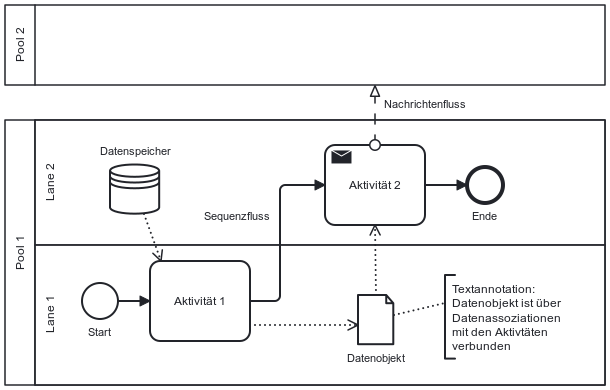
\includegraphics[width=.65\linewidth]{images/process-models/bpmn-elements-showcase}
    \caption{Die relevanten BPMN Elemente in Beziehungen zueinander}
    \label{fig:bpmn-elements-showcase}
\end{figure}

Für die Identifikation von \ac{DSGVO}-kritischen Aktivitäten sind insbesondere folgende Elemente relevant, da sie Hinweise auf den Umgang mit (personenbezogenen) Daten geben. Sie sind ebenfalls in Abbildung \ref{fig:bpmn-elements-showcase} dargestellt:

\begin{itemize}
    \item \textbf{Aktivitäten} bilden die auszuführenden Arbeitsschritte eines Prozesses ab. Sie können Ein- und Ausgaben sowie Datenabhängigkeiten definieren \cite{omgbpmn}. Durch ihren Namen oder Kontext können Rückschlüsse auf die Verarbeitung personenbezogener Daten gezogen werden.
    \item \textbf{Sequenzflüsse} verbinden Aktivitäten, Ereignisse und Gateways und zeigen die Reihenfolge der Ausführung im Prozess an \cite{omgbpmn}. Mit ihrer Hilfe kann eine einzelne Aktivität im Kontext des gesamten Prozesses betrachtet werden, indem der Pfad zu und von der Aktivität verfolgt wird.
    \item \textbf{Datenobjekte und Datenspeicher} repräsentieren flüchtige oder persistente Daten, die im Prozess von z.\,B. Aktivitäten genutzt oder geschrieben werden können \cite{omgbpmn}. Sie können auch personenbezogene Daten enthalten.
    \item \textbf{Datenassoziationen} (Eingangs- und Ausgangsassoziationen) verbinden Aktivitäten mit Datenobjekten und Datenspeichern und zeigen so Ein- und Ausgaben explizit an \cite{omgbpmn}. Sie sind ein wichtiges Signal für die Verarbeitung personenbezogener Daten, da sie den direkten Bezug einer Aktivität zu bestimmten Daten verdeutlichen, z.\,B. Lesezugriff auf eine Kundendatenbank.
    \item \textbf{Pools} modellieren Organisationseinheiten oder Prozessbeteiligte, während \textbf{Lanes} Verantwortlichkeiten innerhalb eines Pools darstellen. Innerhalb eines Pools befinden sich die Aktivitäten und anderen Elemente des Prozesses \cite{omgbpmn}. Die Rollen und Verantwortlichkeiten, die durch Pools und Lanes dargestellt werden, können für die Bewertung der Datenverarbeitung relevant sein.
    \item \textbf{Nachrichtenflüsse} stellen den Austausch von Nachrichten zwischen verschiedenen Pools dar \cite{omgbpmn}. Sie können auf eine Übermittlung personenbezogener Daten an Dritte hinweisen (z.\,B. Transfer von Kundendaten an einen externen Dienstleister).
    \item \textbf{Textannotationen und Assoziationen} dienen dazu, zusätzliche Informationen zu Prozessmodellen hinzuzufügen, die nicht durch die standardmäßigen BPMN-Elemente abgedeckt sind \cite{omgbpmn}. Sie können genutzt werden, um die Art der Datenverarbeitung zu präzisieren, z.\,B. \enquote{enthält E-Mail-Adresse}.
\end{itemize}

\subsection*{\ac{BPMN}-XML}

\ac{BPMN}-Modelle werden in einer XML-Serialisierung, der \ac{BPMN} 2.0 XML, gespeichert \cite{omgbpmn}. Diese Darstellung enthält alle relevanten Strukturinformationen, wie Elementtypen, Namen, Beziehungen, Zuordnungen, Positionen der Elemente, und wird von vielen Prozess-Engines und Modellierungswerkzeugen wie Camunda \cite{camunda} und BPMN.io \cite{bpmnio} unterstützt. Für diese Arbeit dient \ac{BPMN}-XML als Eingabeformat der Klassifizierungspipeline (siehe Kapitel \ref{ch:klassifizierungsalgorithmus-(design-und-implementierung)}).

Jedes \ac{BPMN}-Element hat ein eindeutiges \texttt{id}-Attribut, das als eindeutige Referenzierung dient \cite{omgbpmn}. Diese stabile \texttt{id} ist für die Klassifizierungspipeline wichtig, da sie eine stabile Referenzierung der Aktivitäten und anderer Elemente ermöglicht. Dies ist insbesondere dann relevant, wenn die Ergebnisse der Klassifizierung auf die ursprünglichen Prozessmodelle zurückgeführt werden müssen.

\subsection*{Beispiel einer Datenassoziation als Datenschutzsignal}

Abbildung \ref{fig:data-association-gdpr-example} zeigt ein einfaches Beispiel, wie eine Datenassoziation die \ac{DSGVO}-Relevanz einer Aktivität verdeutlichen kann. In Abbildung \ref{fig:without-data-association} ist die Aktivität \enquote{Daten prüfen} ohne Datenassoziation dargestellt, was wenig über die Art der verarbeiteten Daten aussagt. In Abbildung \ref{fig:with-data-association} hingegen zeigt die eingehende Datenassoziation von einem Datenspeicher \enquote{Kunden-DB}, dass die Aktivität personenbezogene Daten verarbeitet. Dies macht die Aktivität als potenziell datenschutzkritisch erkennbar. Dieses Beispiel unterstreicht die Notwendigkeit den gesamten Kontext einer Aktivität zu betrachten, um fundierte Rückschlüsse auf die Verarbeitung personenbezogener Daten ziehen zu können.

\begin{figure}[h]
    \centering
    \begin{subfigure}{.5\textwidth}
        \centering
        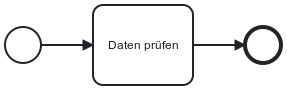
\includegraphics[width=.7\linewidth]{images/process-models/data-association-example-uncritical}
        \caption{Ohne Datenassoziation}
        \label{fig:without-data-association}
    \end{subfigure}%
    \begin{subfigure}{.5\textwidth}
        \centering
        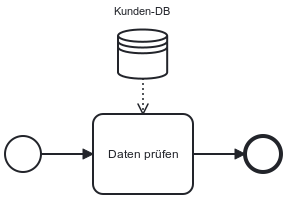
\includegraphics[width=.7\linewidth]{images/process-models/data-association-example-critical}
        \caption{Mit Datenassoziation}
        \label{fig:with-data-association}
    \end{subfigure}
    \caption{Beispiel einer Datenassoziation als Datenschutzsignal}
    \label{fig:data-association-gdpr-example}
\end{figure}
\section{Large Language Models (LLMs)}\label{sec:llms}

\acp{LLM} sind große, vortrainierte Sprachmodelle, die auf der Transformer-Architektur basieren. Transformer, erstmals von Vaswani et al. \cite{vaswani2017attention} beschrieben, verarbeiten eine textuelle Eingabe nicht strikt sequenziell, sondern beachten alle Tokens einer Sequenz parallel. Über sogenannte \texttt{Self-Attention} gewichten sie, welche Token füreinander relevant sind. Als Token gelten Wörter oder Wortbestandteile, in die der Text vorab zerlegt wird. Dieser Attention-Mechanismus erfasst Abhängigkeiten über große Distanzen innerhalb der Sequenz und ermöglicht dadurch eine effiziente Kontextmodellierung, was das zentrale Prinzip moderner \acp{LLM} darstellt. Die Transformer-Architektur bildet heute das Fundament moderner Sprachmodelle wie der GPT-Familie von OpenAI \cite{ibm-gpt, minaee2025largelanguagemodelssurvey, openai-models}, die durch ChatGPT breite Anwendung finden.

In chatbasierten Systemen wird das Verhalten des \ac{LLM} über System- und User-Prompts gesteuert. Gutes Prompt Engineering kann die Leistung und Format-Treue der Ausgabe verbessern, ohne dass die Modellparameter verändert werden müssen \cite{liu2023prompting}. Ein deutlicher Vorteil aktueller \acp{LLM} ist Zero-/Few-Shot Learning. Damit lassen sich Aufgaben allein über Instruktionen und wenige Beispiele lösen, ohne dass erneutes Training benötigt wird \cite{brown2020fewshot, liu2023prompting}. Das ist besonders nützlich für Klassifikationsaufgaben, bei denen nur wenige gelabelte Beispiele vorliegen, wie etwa die Identifikation von \ac{DSGVO}-kritischen Aktivitäten in Prozessmodellen.

Um \acp{LLM} in automatisierten Pipelines zu integrieren, sind schema-konforme Ausgaben, wie ein gültiges JSON, unerlässlich. In der Praxis gibt es dafür drei Ansätze:

\begin{enumerate}
    \item Klare Angaben über das Ausgabeformat im System- oder User-Prompt \cite{liu2023prompting}.
    \item API-gestützte Mechanismen wie Function Calling oder Structured-Output/\linebreak~JSON-Mode mit Schemaüberprüfung \cite{mistralai_structured_output, openai_function_calling_2023, openai_structured_output}.
    \item Constrained Decoding, das die Generierung auf eine vorgegebene Grammatik beschränkt. Ein Beispiel ist PICARD: Bei jedem Generationsschritt des \ac{LM} werden nur zulässige Tokens ausgewählt \cite{scholak2021picard}.
\end{enumerate}

Typische Fehlerbilder bei der Nutzung von \acp{LLM} sind Halluzinationen. Diese sind plausibel wirkende, aber fehlerhafte Aussagen und Formatfehler, wie z.\,B. ungültiges JSON. In \cite{kalai2025languagemodelshallucinate} wird argumentiert, dass Halluzinationen bereits beim Erstellen des \ac{LLM} durch die Trainings- und Evaluationsmethoden begünstigt werden, die das Modell dazu bringen, eher zu raten als Unsicherheit zuzugeben. Das Raten bei Unsicherheit verbessert die Testergebnisse. Gegenmaßnahmen gegen Halluzinationen sind u.a. präzisere Prompts, Informationserweiterung des Prompts durch \ac{RAG} und Self-Check/Retry-Strategien als Post-Processing Methoden nach der Generierung \cite{ji2023hallucinationsurvey}.

Die meisten großen \acp{LLM} werden von Unternehmen wie OpenAI, Google oder Anthropic entwickelt und als API-Dienste angeboten. In der Industrie zählt \texttt{GPT-4o} aktuell zu den am weit verbreitetsten Modellen \cite{openai-hello-gpt-4o}. Es ist ein multimodales Modell mit starken Text-, Bild- und Audiofähigkeiten. Proprietäre Modelle wie GPT-4o sind leistungsfähig, bringen jedoch mehrere Nachteile mit sich. Dazu zählen hohe Kosten und mangelnde Transparenz. Außerdem erfolgt die Datenverarbeitung serverseitig auf Infrastruktur der Anbieter, die sich teils außerhalb der \ac{EU} befindet, wo die \ac{DSGVO} nicht gilt. Für die Verarbeitung personenbezogener Daten innerhalb der \ac{EU} ist das problematisch. Eine Übermittlung in Drittländer ist nur zulässig, wenn dort der Auftragsverarbeiter sämtliche Vorgaben aus Kapitel~5 (Art.~44-50) der \ac{DSGVO} einhält \cite{GDPR2016}.

Als Alternative zu proprietären Modellen steht eine wachsende Zahl frei verfügbarer Open-Source-\acp{LLM} zur Verfügung, die auch lokal betrieben werden können. Prominente Beispiele sind die Modelle von Mistral \cite{mistralai}, Deepseek \cite{deepseek} und Qwen \cite{qwen}. Der lokale Betrieb ermöglicht volle Kontrolle darüber, wo und wie Daten verarbeitet werden. Das erleichtert die Einhaltung datenschutzrechtlicher Anforderungen. Zudem bieten Open-Source-Modelle weitere Vorteile wie geringere Kosten und hohe Anpassbarkeit. In dieser Arbeit werden sowohl proprietäre als auch Open-Source-\acp{LLM} evaluiert (siehe Kapitel \ref{ch:modellauswahl}).
\section{Verwandte Arbeiten}\label{sec:verwandte-arbeiten}

Dieses Kapitel bündelt Arbeiten zur automatisierten \emph{Klassifikation datenschutzkritischer Aktivitäten} in Geschäftsprozessen und zur \emph{Nutzung von \acp{LLM}} in Datenschutzaufgaben und Tätigkeiten im \ac{BPM}. Im Fokus stehen (1) frühe Klassifikations- und Modellierungsansätze, (2) \ac{LLM}-basierte Analyse von Richtlinientexten bis hin zu strukturierter Extraktion, (3) Qualitätssicherung, Prompting und Reproduzierbarkeit, sowie (4) der Einsatz von \acp{LLM} im \ac{BPM}-Lebenszyklus. Abschließend werden Forschungslücken abgeleitet.

\subsection*{Frühe Ansätze: Klassifikation und modellbasierte Kennzeichnung}

Die Identifikation von Prozessschritten mit Verarbeitung personenbezogener Daten ist Voraussetzung wirksamer \ac{DSGVO}-Konformität, da nur so technische und organisatorische Maßnahmen gemäß Art.~32 Abs.~1 \ac{DSGVO} (Vertraulichkeit, Integrität, Verfügbarkeit, Belastbarkeit) zielgerichtet festgelegt werden können \cite{GDPR2016}. Nake et al.\ \cite{nake2023towards} beschreiben einen ersten automatisierten Ansatz: Mit einem überwachten Verfahren (Lernen aus gelabelten Beispielen) klassifizieren sie Aktivitäten in \emph{textuellen} Prozessbeschreibungen als \ac{DSGVO}-kritisch vs.\ unkritisch. Der Datensatz umfasst 37 Prozesse mit 509 Aktivitäten. In der stärksten Konfiguration werden ein F1-Score von $0{,}81$ und ein Recall von $0{,}83$ erreicht. Die Generalisierbarkeit bleibt aufgrund des kleinen, nicht repräsentativen Datensatzes begrenzt. Fehler entstehen u.\,a.\ durch zu wenige Trainingsbeispiele für bestimmte Merkmalswerte. Der Ansatz ist daher als Assistenz für Datenschutzbeauftragte zu verstehen, nicht als vollständige Automatisierung.

Komplementär markieren Capodieci et al.\ \cite{Capodieci2023BPMNEnabledDP} \ac{BPMN}-Elemente mit \ac{DSGVO}-\linebreak~Metadaten via \emph{Tagged Values} (\texttt{GDPR:legalbasis}, \texttt{GDPR:Duration},\linebreak~\texttt{GDPR:risklevel}, \texttt{GDPR:ispersonaldataprocessing}/\texttt{GDPR:personaldata}),\linebreak~sodass Datenschutzaspekte bereits vor der Implementierung der Geschäftsprozesse prüfbar werden. In eine ähnliche Richtung zielt die designorientierte Arbeit von Agostinelli et al.\ \cite{agostinelli2019achievingGDPRComliance}, die \ac{DSGVO}-Anforderungen als wiederverwendbare Muster (\enquote{Data Breach}, \enquote{Consent to Use the Data}, \enquote{Right to Access/Rectify}, \enquote{Portability}, \enquote{Right to be Forgotten}) für eine transparente Einbettung in \ac{BPMN} formalisiert.

\subsection*{\acp{LLM} für Policy-Analyse}

Ciaramella et al.\ \cite{ciaramella2022leveraging} nutzen BERT, RoBERTa und DistilBERT, um Sätze aus Online-Datenschutzerklärungen gezielt im Hinblick auf die Informationspflicht aus Art.~13 (2)(b) \ac{DSGVO} (Hinweis auf Berichtigung/Löschung) zu klassifizieren. Die Ergebnisse sind \emph{moderat} und zeigen, dass innerhalb einer Erklärung konforme und nicht konforme Passagen koexistieren. Daher schließen sie daraus, dass Konformität kein binäres Gesamteurteil nur auf Textebene ist.

Neuere Arbeiten gehen darüber hinaus: Hooda et al.\ \cite{hooda2024policylr} stellen mit \emph{PolicyLR} eine logikbasierte Repräsentation von Richtlinien vor und übersetzen Richtlinientexte mit einem zweistufigen \ac{LLM}-Compiler (Übersetzung $\to$ Entailment-Prüfung) in atomare Formeln. Als Evaluationsbasis dient \emph{ToS;DR} (Terms of Service; Didn’t Read),\linebreak~eine communitybetriebene Plattform, auf der Freiwillige Passagen aus\linebreak~Nutzungs- und Datenschutzerklärungen mit prägnanten \emph{Cases} zu Datenpraktiken annotieren (z.\,B. \enquote{Sie können Ihren Inhalt von diesem Dienst löschen}). Der Compiler extrahiert solche Cases aus Richtlinientexten und prüft anschließend, ob sie logisch aus dem Text folgen (\emph{entailment}). Mit \texttt{gemma2-27b} erreicht der PolicyLR-Compiler eine Precision von $0{,}84$ bei einem Recall von $0{,}88$. Damit werden Com-\linebreak~pliance-Checks, Konsistenzprüfungen und Vergleiche von Datenschutzerklärungen auf Basis formaler Repräsentationen möglich.

Rodriguez et al.\ \cite{rodriguez2024largelanguagemodels} optimieren Prompts, Parameter und die Kontextaufteilung (Chunking) für die feingranulare Extraktion von Erhebungs- und Weitergabepraktiken mit \texttt{GPT-4~Turbo}. Auf MAPP erreichen sie $0{,}935$ F1-Score, auf OPP-115 $0{,}93$ F1-Score, $0{,}949$ Precision, $0{,}912$ Recall und $0{,}904$ Accuracy, während \texttt{Llama-2-70B-Chat} mit $0{,}882$ F1 leicht darunter liegt.

\subsection*{Qualitätssicherung, Prompting und Reproduzierbarkeit}

Zur Reduktion von Halluzinationen koppeln Silva et al.\ \cite{silva2024entailment} einen erklärenden \ac{LLM}-Klassifikator mit einem Entailment-Prüfer, der nur Entscheidungen passieren lässt, die sich aus dem Text folgern lassen. Auf OPP-115 steigt der Macro-F1-Score auf $0{,}63$ (plus $11{,}2$\%). Die zusätzliche Prüfstufe erhöht die Precision von $0{,}38$ auf $0{,}61$, senkt aber den Recall von $0{,}85$ auf $0{,}61$. Für Screening-Aufgaben mit nachgelagerter menschlicher Prüfung eignet sich der Entailment-Schritt damit eher als optionaler High-Precision-Filter. Prompting wirkt als weiterer Qualitätshebel: Von Zero-/Few-Shot-Grundlagen \cite{brown2020fewshot,liu2023prompting} über RoPA-Generierung \cite{pragyan2024toward} bis zu domänenspezifischen Kategorien \cite{schwerin2024systematic} zeigt sich, dass Beispielanzahl, Kontextaufbereitung und Modellwahl entscheidend sind. Reimers und Gurevych \cite{reimers2017reporting} empfehlen zudem, aufgrund seed-bedingter Varianz Score-Verteilungen statt Einzelwerte zu berichten.

\subsection*{\acp{LLM} im BPM-Lebenszyklus}

Über Richtlinientexte hinaus skizzieren Vidgof et al.\ \cite{vidgof2023largelanguagemodelsbusiness} zentrale Forschungsrichtungen für \ac{LLM}-gestütztes \ac{BPM}, darunter Best Practices, \ac{BPM}-spezifische Datensätze und Leitlinien zu Prompting und Modellauswahl. Kourani et al.\ \cite{kourani2025evaluating} vergleichen in einem Benchmark mit 20 Prozessen 16 \acp{LLM} zur Transformation von Prozessbeschreibungen in ausführbare Modelle. \texttt{Claude-3.5-Sonnet} erzielt die höchste durchschnittliche Qualitätsbewertung, während z.\,B.\ \texttt{Mixtral-8x22B} zurückfällt. Es wird ein positiver Zusammenhang zwischen Fehlerbehandlung und Modellqualität beobachtet und, dass durch Output-Optimierungstechniken schwächere Modelle spürbar verbessert werden können. Für dialogorientierte Unterstützung kombinieren Bernardi et al.\ \cite{bernardi2024conversing} \ac{RAG} mit feingetunten \texttt{LLaMA-2}-Modellen (BPLLM) und erreichen bei ausreichender Kontextabdeckung präzise Antworten zu Aktivitäten und Sequenzflüssen.

\subsection*{Forschungslücken}

Aus der Literatur ergeben sich mehrere offene Fragen, die die vorliegende Arbeit adressiert:

\begin{enumerate}
    \item \textbf{Granularität und Domänenfokus.} Viele Studien fokussieren einzelne Artikel der \ac{DSGVO} (z.\,B.\ Art.~13) oder allgemeine Privacy-Tasks. Eine systematische Klassifikation \emph{kompletter} Geschäftsprozesse nach datenschutzrelevanten Aktivitäten ist selten. Zudem sind Datensätze klein und wenig repräsentativ \cite{nake2023towards}.
    \item \textbf{\ac{LLM}-Anwendung in Geschäftsprozessen.} Während es Benchmarks für Prozessmodellierung gibt, fehlen reproduzierbare Benchmarks speziell für die Klassifikation datenschutzkritischer Prozessschritte. Positionsarbeiten wie\linebreak~Vidgof et al.\ \cite{vidgof2023largelanguagemodelsbusiness} fordern \ac{BPM}-spezifische Datensätze und Modelle. Öffentlich verfügbare, auf den europäischen Rechtsraum zugeschnittene Benchmarks sind rar.
    \item \textbf{Erklärbarkeit und Halluzinationen.} \acp{LLM} erzeugen teils überzeugende, aber unzutreffende Ausgaben. Ansätze wie Silva et al.\ \cite{silva2024entailment} und Hooda et al.\ \cite{hooda2024policylr} zeigen, dass Schlussfolgerungsprüfer oder formale Repräsentationen nötig sind, um Halluzinationen zu reduzieren.
    \item \textbf{Datenschutz- und Sicherheitsbedenken.} Studien nutzen häufig geschlossene Modelle wie \texttt{GPT-4}, deren Einsatz aufgrund möglicher Datenübermittlungen in die USA datenschutzrechtlich problematisch sein kann. Offene Modelle wie \texttt{Qwen2-7B} liefern vergleichbare Ergebnisse \cite{schwerin2024systematic} und sind für \ac{EU}-Organisationen potenziell vorteilhaft.
    \item \textbf{Prompt-Engineering-Leitlinien.} Obwohl mehrere Arbeiten den maßgeblichen Einfluss von Prompt-Gestaltung (z.\,B.\ Beispielanzahl, Kontexttrennung) belegen \cite{liu2023prompting,pragyan2024toward}, fehlen breit akzeptierte Leitfäden speziell für Datenschutz- und \ac{BPM}-Kontexte.
\end{enumerate}

Diese Lücken unterstreichen den Bedarf an umfassenden, reproduzierbaren Benchmarks sowie an robusten Methoden zur Klassifikation datenschutzkritischer Aktivitäten in Geschäftsprozessen unter Berücksichtigung der europäischen \ac{DSGVO}. Das folgende Kapitel präzisiert die Problemdefinition und die Qualitätsziele der vorliegenden Arbeit.


\chapter{Problemdefinition und Zielkriterien}\label{ch:problemdefinition-und-zielkriterien}

Ausgehend von den in Kapitel \ref{ch:einleitung} beschriebenen unternehmensweiten, kundenbezogenen Geschäftsprozessen mit personenbezogenen Daten und hohem manuellem Prüfaufwand sowie den Grundlagen zu \ac{DSGVO}, \ac{BPMN} und \acp{LLM} führt dieses Kapitel zur Kernaufgabe: der binären Klassifikation einzelner \ac{BPMN}-Aktivitäten in \emph{kritisch} und \emph{unkritisch} mithilfe von \acp{LLM}. Es definiert die Qualitätsziele und den fachlichen Geltungsbereich und beschreibt das Experimentdesign zur systematischen Beantwortung der Forschungsfragen. Damit legt es die Grundlage für die in Kapitel~\ref{ch:klassifizierungsalgorithmus-(design-und-implementierung)} dargestellte Klassifizierungspipeline sowie für die anschließenden Experimente und deren Auswertung.

Abbildung \ref{fig:running_example} zeigt einen Beispielprozess, der in den folgenden Abschnitten als laufendes Beispiel dient.

\begin{figure}[h]
    \centering
    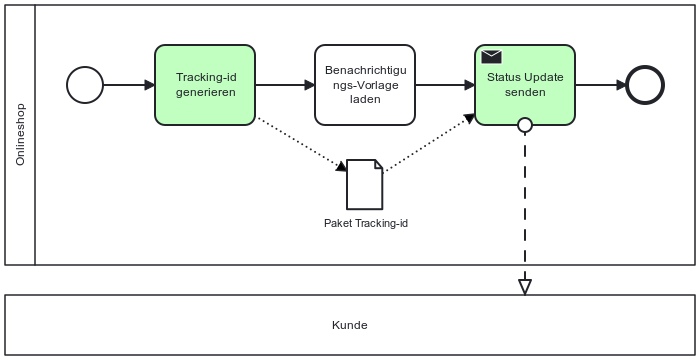
\includegraphics[width=0.7\textwidth]{images/running_example}
    \caption{Beispielprozess zur Veranschaulichung der Aufgabenstellung}
    \label{fig:running_example}
\end{figure}

Der Prozess modelliert den Versand eines Statusberichts eines Onlineshops an Kunden. Dabei werden personenbezogene Daten in den Aktivitäten \enquote{Tracking-id generieren} und \enquote{Status Update senden} verarbeitet, die die stabilen \texttt{ids} \texttt{Activity\_\linebreak~generate} und \texttt{Activity\_send} besitzen. Die Aktivität \enquote{Benachrichtigungsvorlage laden}, mit der \texttt{id} \texttt{Activity\_template}, dient als Negativbeispiel.

\section{Aufgabenstellung}\label{sec:aufgabenstellung}

Ziel der Arbeit ist eine \emph{binäre Klassifikation} auf Ebene einzelner \ac{BPMN}-Aktivitäten: Für jede Aktivität eines Eingabemodells im \ac{BPMN}-XML-Format (Version 2.0.2) \cite{omgbpmn} soll entschieden werden, ob sie \emph{kritisch} im Sinne des Datenschutzrechts ist oder nicht.

\begin{itemize}
    \item \textbf{Eingabe} ist ein valides \ac{BPMN}-XML mit stabilen \texttt{id}-Attributen je Aktivität \cite{omgbpmn}.
    \item \textbf{Ausgabe} ist eine Menge von Aktivitäts-\texttt{ids}, die als \emph{kritisch} klassifiziert worden sind. Optional kann zusätzlich eine natürlichsprachige Begründung für einzelne Entscheidungen ausgegeben werden. Im Fall der Klassifizierungspipeline dieser Arbeit werden die Begründungen vom \ac{LLM} generiert. Die Erklärungen dienen ausschlißelich der Nachvollziehbarkeit der gewählten Klassifizierungen, werden allerdings nicht in der Evaluation berücksichtigt.
\end{itemize}

\subsection*{Begriffsbestimmung \enquote{kritisch}}

Eine Aktivität gilt in dieser Arbeit als \emph{kritisch}, wenn sie \emph{personenbezogene Daten} verarbeitet.Nach Art.~4~Abs.~1 \ac{DSGVO} sind personenbezogene Daten alle Informationen, die sich auf eine identifizierte oder identifizierbare natürliche Person beziehen, und \emph{Verarbeitung} umfasst gemäß Art-~4~Abs.~2 jede mit personenbezogenen Daten vorgenommene Operation (u.\,a. Erheben, Speichern, Abrufen, Verwenden, Übermitteln, Löschen) \cite{GDPR2016}. Dies schließt auch die \emph{Nutzung bereits vorhandener Daten} (z.\,B. Lesen/Abgleichen) ein.
Die Aufgabenstellung reiht sich damit in verwandte Arbeiten ein, die kritische/unkritische Tätigkeiten in Prozessartefakten kennzeichnen (z.\,B. für textuelle Prozessbeschreibungen) \cite{nake2023towards}.
\section{Qualitätsziele}\label{sec:qualitatsziele}

Die Aufgabe der datenschutzrechtlichen Klassifikation von Prozessen ist risikosensitiv. Übersehene kritische Aktivitäten, auch \acp{FN} genannt, bergen erhebliche Compliance-Risiken und können zu hohen Strafen nach der \ac{DSGVO} führen. Beispielsweise erhielt Meta Platforms Ireland Limited (Meta IE) 2023 aufgrund von rechtswidriger Übermittlung von \ac{EU} Nutzerdaten in die USA eine Geldbuße von 1,2 Milliarden Euro \cite{edpb-meta-fine}. Auch Amazon wurde 2025 nach einem langjährigen Rechtsstreit wegen Datenschutzverstößen mit 746 Millionen Euro bestraft \cite{datenschutzticker-amazon-fine, reuters-amazon-fine}. Um derartige Strafen zu vermeiden, müssen kritische Aktivitäten zuverlässig identifiziert werden. Daher ist das \textbf{Hauptziel} der Klassifikation:

\begin{hauptzielbox}
    \textbf{Maximaler Recall} bei \emph{minimalen \acp{FN}} und zugleich \emph{akzeptabler Precision}, damit der manuelle Prüfaufwand durch \acp{FP} begrenzt bleibt.
\end{hauptzielbox}

\subsection*{Konfusionsmatrix und Metriken}

Zur Bewertung des Hauptziels wird eine Konfusionsmatrix verwendet. Im vorliegenden binären Kontext entspricht die positive Klasse \ac{DSGVO}-kritischen Aktivitäten. Die vier Felder der Konfusionsmatrix haben folgende Bedeutung \cite{sokolova2009measureclassification}:

\begin{description}
    \item [\acp{TP}] sind korrekt als kritisch erkannte Aktivitäten. Sie bilden den unmittelbaren \emph{Nutzen} der Klassifikation.
    \item [\acp{FP}] sind fälschlich als kritisch markierte Aktivitäten. Sie erhöhen den manuellen Prüfaufwand, verursachen aber \emph{keine} unmittelbaren Compliance-Risiken.
    \item[\acp{TN}] sind korrekt als unkritisch eingestufte Aktivitäten und reduzieren den Gesamtaufwand.
    \item[\acp{FN}] sind übersehene kritische Aktivitäten. Sie sind besonders problematisch, da sie zu ausbleibender Risikobehandlung und potenziellen Bußgeldern führen können \cite{nake2023towards}.
\end{description}

Aus diesen Größen leiten sich die Evaluationsmetriken ab. Relevante Metriken für eine aussagekräftige Evaluierung sind \emph{Accuracy}, \emph{Precision}, \emph{Recall}, \emph{F1-Score} sowie die Konfusionsmatrix-Zahlen (\acp{TP}, \acp{FP}, \acp{TN}, \acp{FN}) und die Anzahl korrekt/inkorrekt klassifizierter Testfälle. Technische Fehler wie z.\,B. Parsing-Fehler oder überschrittene Token Limits werden separat ausgewiesen.

Diese Metriken sind in Information Retrieval und maschinellem Lernen seit langem etabliert und bilden den De-facto-Standard zur Bewertung von Klassifikatoren \cite{manning2008ir, nake2023towards, sokolova2009measureclassification}. Für das hier betrachtete binäre Problem gelten:

\[
    \mathrm{Accuracy}=\frac{\mathrm{TP}+\mathrm{TN}}{\mathrm{TP}+\mathrm{FP}+\mathrm{TN}+\mathrm{FN}},\quad
    \mathrm{Precision}=\frac{\mathrm{TP}}{\mathrm{TP}+\mathrm{FP}},\quad
\]
\vspace{0.5em}
\[
    \mathrm{Recall}=\frac{\mathrm{TP}}{\mathrm{TP}+\mathrm{FN}},\quad
    \mathrm{F1\mathchar`-Score}=2\cdot\frac{\mathrm{Precision}\cdot \mathrm{Recall}}{\mathrm{Precision}+\mathrm{Recall}}.
\]

\subsection*{Zielwerte}

Vor dem Hintergrund der oben definierten Metriken und dem Hauptziel werden im Folgenden mithilfe von vergleichbarer Literatur realistische Zielkorridore abgeleitet.

Ähnliche Arbeiten, wie von Nake et al. \cite{nake2023towards}, zeigen Referenzwerte von einem maximalen \emph{Recall} $\approx 0{,}83$ und \emph{F1-Score} $\approx 0{,}81$ bei der Identifikation \ac{DSGVO}-kritischer Aufgaben in Prozessbeschreibungen. Jüngere \ac{DSGVO}-nahe \ac{LLM}-Studien berichten von \emph{Precision/Recall} im hohen 0{,}8x bis 0{,}9x-Bereich \cite{hooda2024policylr} und F1-Scores von $\approx 0{,}68$~bis zu $\approx 0{,}79$~\cite{schwerin2024systematic}.

Basierend darauf werden folgende Zielkorridore als \emph{pragmatische Abnahmekriterien} gesetzt:

\begin{itemize}
    \item \textbf{Recall} soll ein Mindestniveau von $\geq 0{,}80$ erreichen und ein \emph{angestrebter} Bereich ist $\geq 0{,}85$.
    \item \textbf{Precision} soll $\geq 0{,}75$ als Untergrenze zur Begrenzung des Prüfaufwands erreichen.
    \item \textbf{F1-Score} soll $\geq 0{,}80$ erreichen.
\end{itemize}

Im Kontext des laufenden Beispiels bedeutet dies u.\,a.: Eine Strategie \enquote{alles ist kritisch} liefert zwar Recall $=1{,}0$, unterschreitet mit Precision $\approx 0{,}67$ jedoch das Ziel. Stattdessen ist daher eine ausgewogene Erkennung gefordert, die \texttt{Activity\_\linebreak~template} korrekt als unkritisch belässt.

Nake~et~al.\ \cite{nake2023towards} zeigen, dass selbst ein \emph{Recall} von $0{,}83$ für kritische Aufgaben ohne menschliche Nachkontrolle nicht ausreicht, da die Strafen für Nichteinhaltung der \ac{DSGVO} sehr hoch sind. Viel mehr eignet sich ein System mit diesem Recall-Wert für \emph{assistierte} Prüfungen, bei denen die Ergebnisse durch qualifizierte Experten validiert werden. Für ein Screening von Geschäftsprozessen, wie es in dieser Arbeit angestrebt wird, sind die genannten Zielwerte daher als realistisch und praxisrelevant einzuschätzen.

Zusammenfassend fixieren die Zielwerte die angestrebte Performance. Im nächsten Abschnitt wird dargelegt, dass aufgrund der nicht-deterministischen Natur von \acp{LLM} die Ergebnisstabilität über wiederholte Läufe berücksichtigt werden muss.

\subsection*{Stabilität über Wiederholungen}

Da \acp{LLM} nicht-deterministisch sind, ist das Berichten eines einzelnen Leistungswertes nicht ausreichend für den Vergleich von Modellen. Studien wie von Reimers et al. \cite{reimers2017reporting} zeigen, dass die Abhängigkeit vom Seed-Wert der \acp{LLM} zu statistisch signifikanten Unterschieden in der Performance führen kann. Diese Varianz kann dazu führen, dass ein modernes, leistungsfähiges Modell von sehr gut bis mittelmäßig abschneidet. Stattdessen wird vorgeschlagen, Score-Verteilungen zu vergleichen, die auf mehreren Durchläufen basieren. Dadurch wird das Risiko reduziert, dass ein Modell nur aufgrund eines günstigen Seeds gut oder aufgrund eines ungünstigen Seeds schlecht abschneidet. Im laufenden Beispiel ist \enquote{Generate tracking id} grenzwertig und wird in der Praxis von Modellen gelegentlich fälschlich als \emph{nicht-kritisch} markiert (\ac{FN}) - Wiederholungen und das Berichten von Mittelwert $\pm$ Standardabweichung ($\sigma$) erfassen diese Instabilität.

In dieser Arbeit werden daher die Ergebnisse auf Basis von Wiederholungen berichtet. Es wird der Mittelwert $\pm$ Standardabweichung je Metrik angegeben. Modellvergleiche basieren am Ende auf diesen Verteilungen und nicht auf Einzelfällen.
\section{Scope und Annahmen}\label{sec:scope-und-annahmen}

Dieser Abschnitt definiert Geltungsbereich, Annahmen und Risiken des Ansatzes. Dadurch wird eine klare Einordnung der Ergebnisse und ihrer Reproduzierbarkeit ermöglicht.

\subsection*{Geltungsbereich}

Die folgenden Punkte definieren den Geltungsbereich der Arbeit:

\begin{itemize}
    \item Klassifiziert werden ausschließlich \emph{Aktivitäten}. Dafür wird sinnvoller Kontext berücksichtigt, wie Labels, Pools/Lanes (z.\,B.\ \enquote{Onlineshop}, \enquote{Kunde}), Message Flows sowie vorhandene Datenobjekte (z.\,B.\ \enquote{Paket Tracking-id}).
    \item Labels und Artefakte liegen in Deutsch und Englisch vor.
    \item Es handelt sich um ein \emph{Screening}, nicht um eine Rechtsprüfung. Kritisch klassifizierte Aktivitäten sind anschließend juristisch zu prüfen.
\end{itemize}

\subsection*{Annahmen und Risiken}

Die folgenden Annahmen und potenziellen Risiken sind für die Interpretation der Ergebnisse relevant:

\begin{itemize}
    \item Bei fehlenden Datenobjekten oder mehrdeutigen Labels kann sich die Einschätzung verschlechtern. Das ist ein bekanntes Problem in ähnlichen Studien \cite{nake2023towards}.
    \item Optional generierte \ac{LLM}-Begründungen sind als \emph{Hilfetexte} zu verstehen, um die Entscheidung des \acp{LLM} besser einordnen zu können, bilden aber nicht zwingend die tatsächlichen Entscheidungsgründe des Modells ab.
    \item Ungültiges \ac{BPMN}-XML oder Laufzeitfehler werden als \enquote{technischer Fehler} erfasst und nicht in die Metrikzählung eingerechnet. Sie werden separat berichtet.
\end{itemize}
\section{Experimentdesign}\label{sec:experimentdesign}

Das gesamte Kapitel definierte die binäre Klassifikation von \ac{BPMN}-Aktivitäten als kritisch/unkritisch mit Fokus auf maximalen Recall bei akzeptabler Precision und legte Qualitätsziele, Metriken, Geltungsbereich sowie Annahmen fest. Darauf aufbauend beschreibt dieser Abschnitt das Experimentdesign, mit dem \acp{LLM} fair und reproduzierbar verglichen werden, um die Forschungsfrage \textbf{FF1} sowie die Unterfragen \textbf{UF1}–\textbf{UF4} zu beantworten. Die konkrete Ausgestaltung und Durchführung der Experimente werden in Kapitel \ref{ch:versuchsaufbau-und-durchfuhrung} \emph{Versuchsaufbau} erläutert. Im Folgenden werden die wesentlichen Aspekte des Experimentdesigns beschrieben:

\begin{description}
    \item[\textbf{Ziel}] Ziel ist ein transparenter Vergleich mehrerer \acp{LLM}, die alle dieselbe Klassifizierungspipeline durchlaufen. Sie wird in Kapitel \ref{ch:klassifizierungsalgorithmus-(design-und-implementierung)} daher so entworfen, dass sich das \ac{LLM} austauschen lässt. Die Auswahl der im Evaluationsframework aus Kapitel \ref{ch:evaluationsframework} zu nutzenden \acp{LLM} erfolgt zur Laufzeit anhand übergebener Identifikationsparameter (z.,B. Modellname, Basis-URL/Endpunkt).
    \item[\textbf{Vergleichsgegenstand}] Die Experimente werden über eine deklarative Konfiguration definiert, siehe Kapitel~\ref{sec:konfiguration-einer-evaluierung}. Sie legt fest, welche Modelle, Datensätze und weitere Parameter zum Einsatz kommen. Je nach Auswahl werden mehrere Modelle und Modellvarianten parallel im Evaluationsframework ausgeführt, darunter Open-Source und kommerzielle Modelle. Die deklarative Konfiguration sorgt für Portabilität und Wiederholbarkeit.
    \item[\textbf{Datenbasis}] Als Datenbasis dienen die im Labeling-Tool erzeugten, gelabelten Testdatensätze, siehe Kapitel \ref{ch:labeling-und-datensatze}. Ein Testdatensatz enthält mehrere gelabelte Testfälle. Ein Testfall umfasst ein \ac{BPMN}-Prozessmodell mit Labeln, die Aktivitäten als \ac{DSGVO}-kritisch markieren. Die Auswahl der Datensätze für ein Experiment erfolgt in der Evaluierungskonfiguration und das Laden der Testfälle während der Laufzeit. Die Datensätze sollten idealerweise unterschiedliche Eigenschaften abdecken, damit die Forschungsfrage und die Unterfragen möglichst umfassend beantwortet werden. Unterschiede können sich etwa in der Domäne, der Größe der Prozesse, den eingesetzten Sprachen oder den verwendeten \ac{BPMN}-Elementen zeigen.
    \item[\textbf{Metriken und Erfolgskriterium}] Ausgewertet werden die in Abschnitt~\ref{sec:qualitatsziele} beschriebenen Metriken: Accuracy, Precision, Recall und F1. Zusätzlich werden die Kennzahlen der Konfusionsmatrix betrachtet: \ac{TP}, \ac{FP}, \ac{TN}, \ac{FN}. Ein Testfall gilt als \emph{bestanden}, wenn die vom Modell als kritisch ausgegebenen Aktivitäten exakt den gelabelten kritischen Aktivitäten entsprechen. Technische Fehler werden separat ausgewiesen.
\end{description}

\subsection*{Ablauf eines Experiments}

Ein Experiment verläuft in folgenden Schritten:

\begin{enumerate}
    \item \textbf{Konfiguration laden}. Die Konfiguration mit Modellen, Datensätzen und optionalem \texttt{seed} wird geladen.
    \item \textbf{Ausführung}. Für jedes Modell werden alle ausgewählten Testfälle durch die Klassifizierungspipeline verarbeitet. Pro Testfall werden \ac{TP}, \ac{FP}, \ac{FN}, \ac{TN} sowie der Status \enquote{bestanden} oder \enquote{nicht bestanden} berechnet.
    \item \textbf{Stabilität}. Die Läufe erfolgen mit niedriger \texttt{temperature}\footnote{Die \texttt{temperature} steuert die Zufälligkeit der Textgenerierung bei \acp{LLM}. Niedrige Werte liefern stabilere Antworten, hohe Werte vielfältigere, jedoch weniger verlässliche \cite{ibm-llm-temperature}.} und festem \texttt{seed}, sofern das jeweilige \ac{LLM} dies unterstützt. Um die Nicht-Deterministik moderner \acp{LLM} abzubilden, werden die Experimente mehrfach mit unterschiedlichen Seeds wiederholt. Die Ergebnisse werden über die Läufe gemittelt.
    \item \textbf{Bericht}. Aggregierte Kennzahlen pro Modell, wie Konfusionsmatrix, die genannten Metriken sowie die Bestehensraten werden ausgegeben. Metadaten wie verwendete Modelle, Datensätze und Seeds werden dokumentiert.
\end{enumerate}

Dieses Kapitel definiert, \emph{was} verglichen wird: Modelle, Datensätze und Metriken. Es beschreibt zudem, \emph{wie} der Vergleich erfolgt. Kapitel~\ref{ch:versuchsaufbau-und-durchfuhrung} dokumentiert später die praktische Umsetzung mit konkreten Modellen, exakten Parameterwerten, Seeds sowie den vollständigen genutzten Konfigurationen. Im nächsten Kapitel folgt das Design und die Implementierung der Klassifizierungspipeline, die für den Vergleich der \acp{LLM} verwendet wird.

\chapter{Klassifizierungsalgorithmus (Design und Implementierung)}\label{ch:klassifizierungsalgorithmus-(design-und-implementierung)}

Dieses Kapitel beschreibt die Pipeline zur Klassifikation \ac{DSGVO}-kritischer Aktivitäten in \ac{BPMN}-Prozessen. Ausgehend von der in kapitel \ref{sec:aufgabenstellung} formulierten Aufgabenstellung wird der gesamte Weg von der Eingabe eines \emph{BPMN-XML} über die Vorverarbeitung, das Prompt Engineering bis hin zur strukturierten, schema-konformen Ausgabe aufgezeigt. Außerdem wird ein HTTP-basiertes API-Design vorgestellt, das die Einbindung in weitere Werkzeuge und das Evaluationsframework ermöglicht.

Die Klassifizierungspipeline soll eine binäre Entscheidung auf Ebene einzelner BPMN-Aktivitäten treffen: Für jede Aktivität eines Eingabemodells wird bestimmt, ob sie \emph{kritisch} im Sinne der \ac{DSGVO} ist. Die Pipeline ist so konzipiert, dass sie mit Modellen aus gängigen Modellierungswerkzeugen kompatibel ist.

\section{BPMN Preprocessing}\label{sec:bpmn-preprocessing}

Ziel der Vorverarbeitung (Preprocessing) ist es, für jedes Flow-Element einen \emph{strukturierten Kontext} zu erzeugen. Dieser Kontext umfasst die eigenen Attribute, wie \texttt{id}, \texttt{name} und \texttt{documentation}, sowie die Beziehungen zu anderen Elementen im \ac{BPMN}-Diagramm. Dazu gehören vorangehende und nachfolgende Flow-Elemente, Datenobjekte, assoziierte Elemente, sowie Informationen über den Pool und die Lane, in denen sich das Element befindet. Das Parsen des \ac{BPMN}-XML erfolgt mit der \emph{Camunda BPMN Model API}, die das XML in ein Objektmodell überführt \cite{camunda-bpmn-model-api, camunda-bpmn-model-read}. Auf dieser Basis werden die relevanten Informationen extrahiert und in der Datenklasse \texttt{BpmnElement} strukturiert abgelegt. Die Datenklasse ist in Listing \ref{lst:bpmn-element-class} zu sehen. Dadurch entsteht für jedes Flow-Element ein umfassender Kontext, der später im Prompt genutzt wird, um dem \ac{LLM} alle notwendigen Informationen strukturiert bereitzustellen. Außerdem werden durch das Format Tokens eingespart, da irrelevante Informationen, wie die Positionen der Elemente im XML, weggelassen werden. In Abbildung \ref{fig:architecture-diagram} ist dieser Schritt über die Aktivität \enquote{Kontext aller Elemente aufbauen} dargestellt.

\begin{lstlisting}[language=Kotlin,caption={Interne \ac{BPMN}-Repräsentation je Flow-Element.},label={lst:bpmn-element-class}]
data class BpmnElement(
    val type: String,
    val id: String,
    val name: String? = null,
    val documentation: String? = null,
    val poolName: String? = null,
    val laneName: String? = null,
    val outgoingFlowElementIds: List<String> = emptyList(),
    val incomingFlowElementIds: List<String> = emptyList(),
    val outgoingMessageFlowsToElementIds: List<String> = emptyList(),
    val incomingMessageFlowsFromElementIds: List<String> = emptyList(),
    val incomingDataFromElementIds: List<String> = emptyList(),
    val outgoingDataToElementIds: List<String> = emptyList(),
    val associatedElementIds: List<String> = emptyList()
)
\end{lstlisting}
\section{Prompt Engineering}\label{sec:prompt-engineering}

Eine robuste Klassifikation hängt maßgeblich von sorgfältig gestalteten Prompts ab. Ziel ist es, das \ac{LLM} mit klaren Anweisungen, einem konsistenten Bewertungsschema und präzisen Formatvorgaben so zu steuern, dass es die Klassifizierung zuverlässig löst und strukturierte Ausgaben liefert. Im Folgenden werden zunächst die deklarative Orchestrierung der Kommunikation mit dem \ac{LLM} mithilfe von LangChain4j und anschließend die Prompt-Konzeption beschrieben.

\subsection*{LangChain4j: deklarative Orchestrierung}
Zur Reduktion von Boilerplate und für konsistente Prompts wird \emph{LangChain4j} \cite{langchain4j} benutzt. Mit den \emph{AI Services} werden Interaktionen mit dem \ac{LLM} als Java/Kotlin-Interface \emph{deklarativ} beschrieben. Zur Laufzeit erzeugt LangChain4j einen Proxy, der den System-Prompt injiziert, den User-Prompt aus den Methodenparametern generiert und die \ac{LLM}-Antwort in den passenden Rückgabetyp deserialisiert \cite{langchain4j-ai-services}. Beim erstellen des AI Service werden ein \texttt{ChatModel}, die Systemnachricht und die Interface-Methoden konfiguriert. Ein \texttt{ChatModel} ist die spezifische Implementierung der Chat-Completion-Schnittstelle eines \ac{LLM} von Langchain4j \cite{langchain4j-chat-model}. Die Methodenparameter der Interface-Methoden repräsentieren die Nutzereingabe. Der Rückgabetyp der Methoden definiert die erwartete Antwortstruktur des \ac{LLM}. Optional kann jeder Interface-Methode noch ein eigener User-Prompt zugewiesen werden, der bei Laufzeit mit den übergebenen Parametern gefüllt wird \cite{langchain4j-ai-services}.

Die Kommunikation mit dem \ac{LLM} erfolgt damit über einfache Funktionsaufrufe, während LangChain4j Prompt-Erzeugung, Parameterbindung sowie die Deserialisierung der Antwort übernimmt \cite{langchain4j-ai-services}. So kann im Code ohne zusätzlichen Aufwand direkt mit typisierten Objekten gearbeitet werden.

Für die Klassifikation \emph{\ac{DSGVO}-kritisch vs.\ unkritisch} wird ein \textbf{Zero-Shot}-Ansatz verwendet. Das \ac{LLM} erhält im System-Prompt eine präzise Instruktion mit Kriterien und illustrativen Beispielfällen, was als kritisch gilt. Es sind jedoch keine Beispiele mit konkreten Ein- und Ausgabe-paaren pro Prozess enthalten. Zero-Shot reduziert den Pflegeaufwand und nutzt die In-Context-Fähigkeiten moderner Modelle, nur über Instruktionen zu generalisieren \cite{brown2020fewshot,liu2023prompting}. Wie genau die Prompts aufgebaut sind, wird im Folgenden beschrieben.

\subsection*{System-Prompt}

Der System-Prompt definiert das Verhalten des \ac{LLM}, zusätzlichen Kontext und das gewünschte Ausgabeformat. Der vollständige System-Prompt befindet sich im Anhang, siehe \ref{lst:system-prompt}. Im Kern legt der genutzte System-Prompt Folgendes fest:

\begin{enumerate}
    \item \textbf{Rolle und Auftrag des Modells.} Das Modell agiert als Experte für das Analysieren von \ac{BPMN}-Modellen auf \ac{DSGVO}-konformität und prüft sämtliche Aktivitäten eines Prozesses auf Datenschutzrelevanz. Jede Aktivität wird berücksichtigt und die Entscheidung erfolgt auf Basis sämtlicher verfügbarer Kontextinformationen wie Name, Beschreibung, Annotationen sowie Daten- und Nachrichtenassoziationen.
    \item \textbf{Rechtliche Definitionen nach \ac{DSGVO}.} Der System-Prompt erläutert die Begriffe \enquote{personenbezogene Daten} und \enquote{Verarbeitung} gemäß Art.\,4 \ac{DSGVO}. Beispiele für personenbezogene Daten umfassen Identifikatoren, Kontakt- und Zahlungsdaten, Beschäftigungsdaten, Gesundheitsdaten, biometrische Merkmale, Standortinformationen und Online-Kennungen. Verarbeitung umfasst Erheben, Speichern, Abrufen, Verwenden, Übermitteln, Ausrichten, Kombinieren, Einschränken, Löschen und Vernichten.
    \item \textbf{Indikatoren für Kritikalität.} Der System-Prompt enthält typische Auslöser für Datenschutzrelevanz wie Datenerfassung und Dateneingabe, Anlage und Aktualisierung von Datensätzen, Übermittlung oder Offenlegung an andere Systeme oder Dritte, Zahlungen und Finanztransaktionen und noch mehr. Diese Indikatoren sind mit Beispielen angereichert und dienen als \emph{Entscheidungshelfer} für das Modell.
    \item \textbf{Abgrenzung durch Negativbeispiele.} Der System-Prompt grenzt unkritische Fälle klar ab. Rein administrative oder logistische Schritte ohne Personenbezug werden nicht als kritisch gewertet. Ebenso gilt dies für Fälle in denen anonymisierte Daten verwendet werden und keine Identifikation einer Person mehr möglich ist.
    \item \textbf{Erwartetes Ausgabeformat.} Die Antwort erfolgt als strukturierte JSON-\hspace{0pt}Ausgabe mit einer Liste relevanter Aktivitäten. Für jede Aktivität wird die \texttt{id} und eine Begründung in natürlicher Sprache ausgegeben. Es werden ausschließlich Aktivitäten zurückgegeben, die nach den Kriterien als datenschutzrelevant eingestuft wurden.
\end{enumerate}

Die Kombination dieser Elemente im System-Prompt stellt sicher, dass das \ac{LLM} die Aufgabe versteht, die relevanten Kriterien kennt und die Ausgabe in einem maschinenlesbaren Format liefert. So entsteht die Basis für eine zuverlässige Klassifikation. Zu einer Anfrage an ein \ac{LLM} gehört außerdem stets ein User-Prompt, der die eigentliche Nutzereingabe enthält. Dessen Aufbau wird im nächsten Abschnitt beschrieben.

\subsection*{User-Prompt}

Der User-Prompt übergibt dem \ac{LLM} die konkreten Eingabedaten einer Anfrage. Während der System-Prompt Regeln, Ziele und Ausgabevorgaben festlegt, liefert der User-Prompt die Fall- bzw.\ Kontextinformationen, auf die diese Regeln angewendet werden.

Der User-Prompt wird mithilfe der Daten aus der Vorverarbeitung aus Abschnitt \ref{sec:bpmn-preprocessing} erzeugt und enthält eine Liste von \texttt{BpmnElement}-Objekten, siehe Listing~\ref{lst:bpmn-element-class}. Die Interaktion mit dem \ac{LLM} erfolgt deklarativ über \emph{LangChain4j}. Dafür wird die Liste der \texttt{BpmnElement}-Objekte als Methodenparameter mit der Annotation \texttt{@UserMessage} an die Interface-Methode übergeben und dort automatisch in den User-Prompt eingebettet.

Zur Laufzeit serialisiert \emph{LangChain4j} die \texttt{BpmnElement}-Liste zu einem JSON-Array und stellt sie als User-Prompt bereit. Der zuvor konfigurierte System-Prompt wird bei einer Anfrage an das \ac{LLM} automatisch dem User-Prompt vorangestellt. Auf diese Weise wendet das \ac{LLM} die im System-Prompt definierten Kriterien auf die im User-Prompt gelieferten Informationen zum \ac{BPMN}-Prozessmodell an. Dadurch wird jede Aktivität des Prozesses genau so wie im System-Prompt beschrieben klassifiziert. In Abbildung \ref{fig:architecture-diagram} findet dieser Schritt in der Aktivität \enquote{Anfrage an das LLM schicken} statt.

Zusammenfassend setzt der System-Prompt typischerweise das Regelwerk, und der User-Prompt liefert die konkreten Eingabedaten. Besonders in mehrstufigen Dialogen mit dem \ac{LLM} spielt dieses Muster eine größere Rolle, da der System-Prompt konstant bleibt, während der User-Prompt je nach Anfrage variiert. Im vorliegenden Szenario, wo immer nur genau eine Anfrage pro Prozessmodell gestellt wird fällt der Unterschied weniger ins Gewicht, als würden sämtliche Vorgaben direkt im User-Prompt stehen. Die Trennung erhöht dennoch die Nachvollziehbarkeit, sorgt für klare Rollen und erleichtert die Wiederverwendung.

Im folgenden Abschnitt wird beschrieben, wie auf dieser Basis strukturierte Ausgaben erzeugt werden, damit im Code direkt mit typisierten Objekten weitergearbeitet werden kann.

\subsection*{Strukturierte Ausgaben mit LangChain4j}

Wie in Listing \ref{lst:ai-service-interface} zusehen, wird im Fall der Klassifikation ein \texttt{BpmnAnalysisResult} als Antwort erwartet, also eine Liste von Elementen mit Paaren aus \texttt{id}, \texttt{reason} und \texttt{isRelevant}. Siehe \ref{lst:bpmn-analysis-result} für die vollständige Definition der Datenklasse. Langchain4j inferiert auf Basis des Rückgabetyps der Interface-Methode ein JSON-Schema und fügt dieses automatisch dem User-Prompt zusammen mit der Aufforderung hinzu, die Antwort in diesem JSON-Format zu liefern \cite{langchain4j-ai-services}. Durch die explizite Angabe des gewünschten JSON-Formats im Prompt wird die Format-Treue der Antwort erhöht \cite{liu2023prompting}, also die Wahrscheinlichkeit, dass die Antwort tatsächlich dem gewünschten Schema entspricht.

Einige \acp{LLM} unterstützen darüber hinaus die Möglichkeit, das Antwortformat API-seitig zu erzwingen. Das ist beispielsweise bei Mistral und OpenAI der Fall \cite{mistralai_structured_output, openai_structured_output}.
Falls das \ac{LLM} die \texttt{response\_format} Funktionalität unterstützt setzt LangChain4j dies zusätzlich auf das gewünschte Schema und erzwingt so das Ziel-JSON API-seitig \cite{langchain4j-ai-services}. Fehlt diese Fähigkeit, greift ausschließlich die Prompt-basierte Schemaanweisung.

Das vom \ac{LLM} gelieferte JSON deserialisiert \emph{LangChain4j} anschließend automatisch zu einem \texttt{BpmnAnalysisResult}. So kann im Code direkt mit einem typsicheren Objekt weitergearbeitet werden. In Abbildung \ref{fig:architecture-diagram} ist dieser Prozess über die Aktivitäten \enquote{Antwort von LLM erhalten} und \enquote{Antwort JSON deserialiseren} dargestellt.

\section{Validierung der Ausgabe}\label{sec:validierung-der-ausgabe}

Zusätzlich zu den in Kapitel \ref{sec:prompt-engineering} beschriebenen Maßnahmen zur Sicherstellung strukturierter Ausgaben wird die Antwort des \ac{LLM} durch LangChain4j validiert. Wenn das erwartete Schema vom \ac{LLM} nicht eingehalten wird, wirft Langchain4j eine \texttt{OutputParsingException}.

\textcolor{orange}{// TODO Eventuell noch Retry Mechanismus wenn am Ende noch Zeit ist mit Nachrichtenverlauf und Parsing Fehlermeldung. Das muss aber auch erst einmal implementiert werden. Aktuell gibt es nur den Parsing Error.}

Ein weiterer Mechanismus zur Validierung der Ausgabe ist die Überprüfung der ausgegebenen \texttt{ids}. Da das \ac{LLM} theoretisch jede beliebige \texttt{id} ausgeben könnte, werden die ausgegebenen \texttt{ids} mit den tatsächlichen \texttt{ids} der Aktivitäten aus dem Prozess abgeglichen. Falls eine ausgegebene Aktivität nicht im Prozess existiert, wird diese aus der Antwort der Klassifizierung entfernt. Dadurch wird sichergestellt, dass nur gültige \texttt{ids} in der finalen Ausgabe enthalten sind.
\section{API-Design}\label{sec:api}

Dieses Kapitel beschreibt das API-Design der Klassifizierungspipeline, die zur Erkennung \ac{DSGVO}-kritischer Elemente in \ac{BPMN}-Modellen dient. Das Ziel ist es eine standardisierte Schnittstelle zu definieren, um

\begin{enumerate}
    \item die Einbindung in bestehende Werkzeuge und das Evaluationsframework (siehe Kapitel \ref{ch:evaluationsframework}) zu vereinfachen,
    \item die Austauschbarkeit unterschiedlicher Klassifizierungsalgorithmen - insbesondere im Evaluationsframework - zu ermöglichen, um verschiedene Ansätze vergleichen zu können, und
    \item Erweiterbarkeit zu fördern, sodass zukünftige Arbeiten die Schnittstelle wiederverwenden können, um ihre eigenen Klassifizierungsalgorithmen zu integrieren.
\end{enumerate}

\subsection*{HTTP-Endpunkt}

Die Klassifizierungspipeline ist über einen HTTP-Endpunkt nutzbar. Der \texttt{POST}-Endpunkt akzeptiert \texttt{multipart/form-data} mit den folgenden Teilen:

\begin{description}
    \item[\texttt{bpmnFile} (Pflicht)] Eine BPMN-2.0-XML-Datei (\texttt{.bpmn} oder \texttt{text/xml}), die den zu analysierenden Prozess beinhaltet.
    \item[\texttt{llmProps} (Optional)] Ein JSON-Objekt zur Überschreibung von \ac{LLM}-Eigenschaften zur Laufzeit. Siehe Listing \ref{lst:api-request-schema} für das JSON-Schema. Wird nichts angegeben, nutzt die Pipeline Standardwerte.
\end{description}

Die \texttt{llmProps} erlauben es, verschiedene \acp{LLM} und deren Konfigurationen flexibel zu für die Klassifizierung zu nutzen, ohne die Anwendung neu starten zu müssen. Dies ist besonders nützlich im Evaluationsframework, um verschiedene Modelle zu vergleichen.

\begin{lstlisting}[language=json,caption={JSON-Schema der \texttt{llmProps}.},label={lst:api-request-schema}]
{
  "$schema": "https://json-schema.org/draft/2020-12/schema",
  "title": "LlmProps",
  "type": "object",
  "properties": {
    "baseUrl": {"type": "string"},
    "modelName": { "type": "string" },
    "apiKey": { "type": "string" },
    "timeoutSeconds": { "type": "number" },
    "seed": { "type": "number" }
  },
  "required": []
}
\end{lstlisting}

Die Antwort des Endpunkts wird als \texttt{application/json} geliefert und enthält eine Liste der als \ac{DSGVO}-kritisch klassifizierten Elemente, einschließlich einer optionalen Begründung für jede Klassifikation und einem optionalen Namen des Elements für bessere Lesbarkeit. Das JSON-Schema der API-Antwort ist in Listing \ref{lst:api-response-schema} dargestellt.

\begin{lstlisting}[language=json,caption={JSON-Schema der API-Antwort.},label={lst:api-response-schema}]
{
  "$schema": "https://json-schema.org/draft/2020-12/schema",
  "title": "BpmnAnalysisResult",
  "type": "object",
  "properties": {
    "criticalElements": {
      "type": "array",
      "items": {
        "type": "object",
        "properties": {
          "id": { "type": "string" },
          "name": { "type": "string" },
          "reason": { "type": "string" }
        },
        "required": ["id"]
      }
    }
  },
  "required": ["criticalElements"]
}
\end{lstlisting}

Ein Beispielaufruf des Klassifizierungsendpunkts mit \texttt{curl} könnte wie in Listing \ref{lst:api-curl-example} aussehen. Dabei wird eine BPMN-Datei hochgeladen und einige \ac{LLM}-Eigenschaften zur Laufzeit überschrieben, damit das Modell \texttt{mistral-small-latest} von Mistral AI verwendet wird.

\begin{lstlisting}[language=bash,caption={Beispielaufruf des Klassifizierungsendpunkts mit \texttt{curl}.},label={lst:api-curl-example}]
curl -X POST http://localhost:8080/gdpr/analysis/prompt-engineering \
    -F 'bpmnFile=@/path/to/process.bpmn' \
    -F 'llmProps={
        "baseUrl": "https://api.mistral.ai/v1/chat/completions",
        "modelName": "mistral-small-latest",
        "apiKey": "******"
    }'
\end{lstlisting}

\subsection*{Integration und Erweiterbarkeit}

Die gewählte API-Struktur mit einem standardisierten HTTP-Endpunkt und klar definierten JSON-Schemas ermöglicht eine einfache Integration in bestehende Werkzeuge und das Evaluationsframework (siehe Kapitel \ref{ch:evaluationsframework}). Durch die Möglichkeit, verschiedene \ac{LLM}-Eigenschaften zur Laufzeit zu überschreiben, können unterschiedliche Modelle mit einem Klassifizierungsalgorithmus flexibel getestet und verglichen werden, ohne die Anwendung neu starten zu müssen.

Zukünftige Arbeiten können die gleiche API nutzen, um ihre eigenen Klassifizierungsalgorithmen zu integrieren und so eine Vergleichbarkeit der Ergebnisse zu gewährleisten.
\section{Nutzung über Webapp}\label{sec:nutzung-uber-webapp}

Zur interaktiven Nutzung der Klassifizierung wurde eine \emph{Sandbox} in Form einer Webapp entwickelt. Sie verbindet einen vollwertigen \ac{BPMN}-Editor auf Basis von \texttt{BPMN.js} \cite{bpmn-js} mit der in Kapitel~\ref{sec:api-design} beschriebenen HTTP-Schnittstelle und macht die Analyse damit ganz einfach bedienbar. In der Sandbox können \ac{BPMN}-Modelle erstellt, verändert, exportiert und importiert sowie auf Datenschutzrelevanz analysiert werden. Als kritisch klassifizierte Aktivitäten werden nach der Analyse direkt im Editor farblich hervorgehoben, wie in Abbildung \ref{fig:sandbox-frontend-analyzed-model} zu sehen.

\begin{figure}
    \centering
    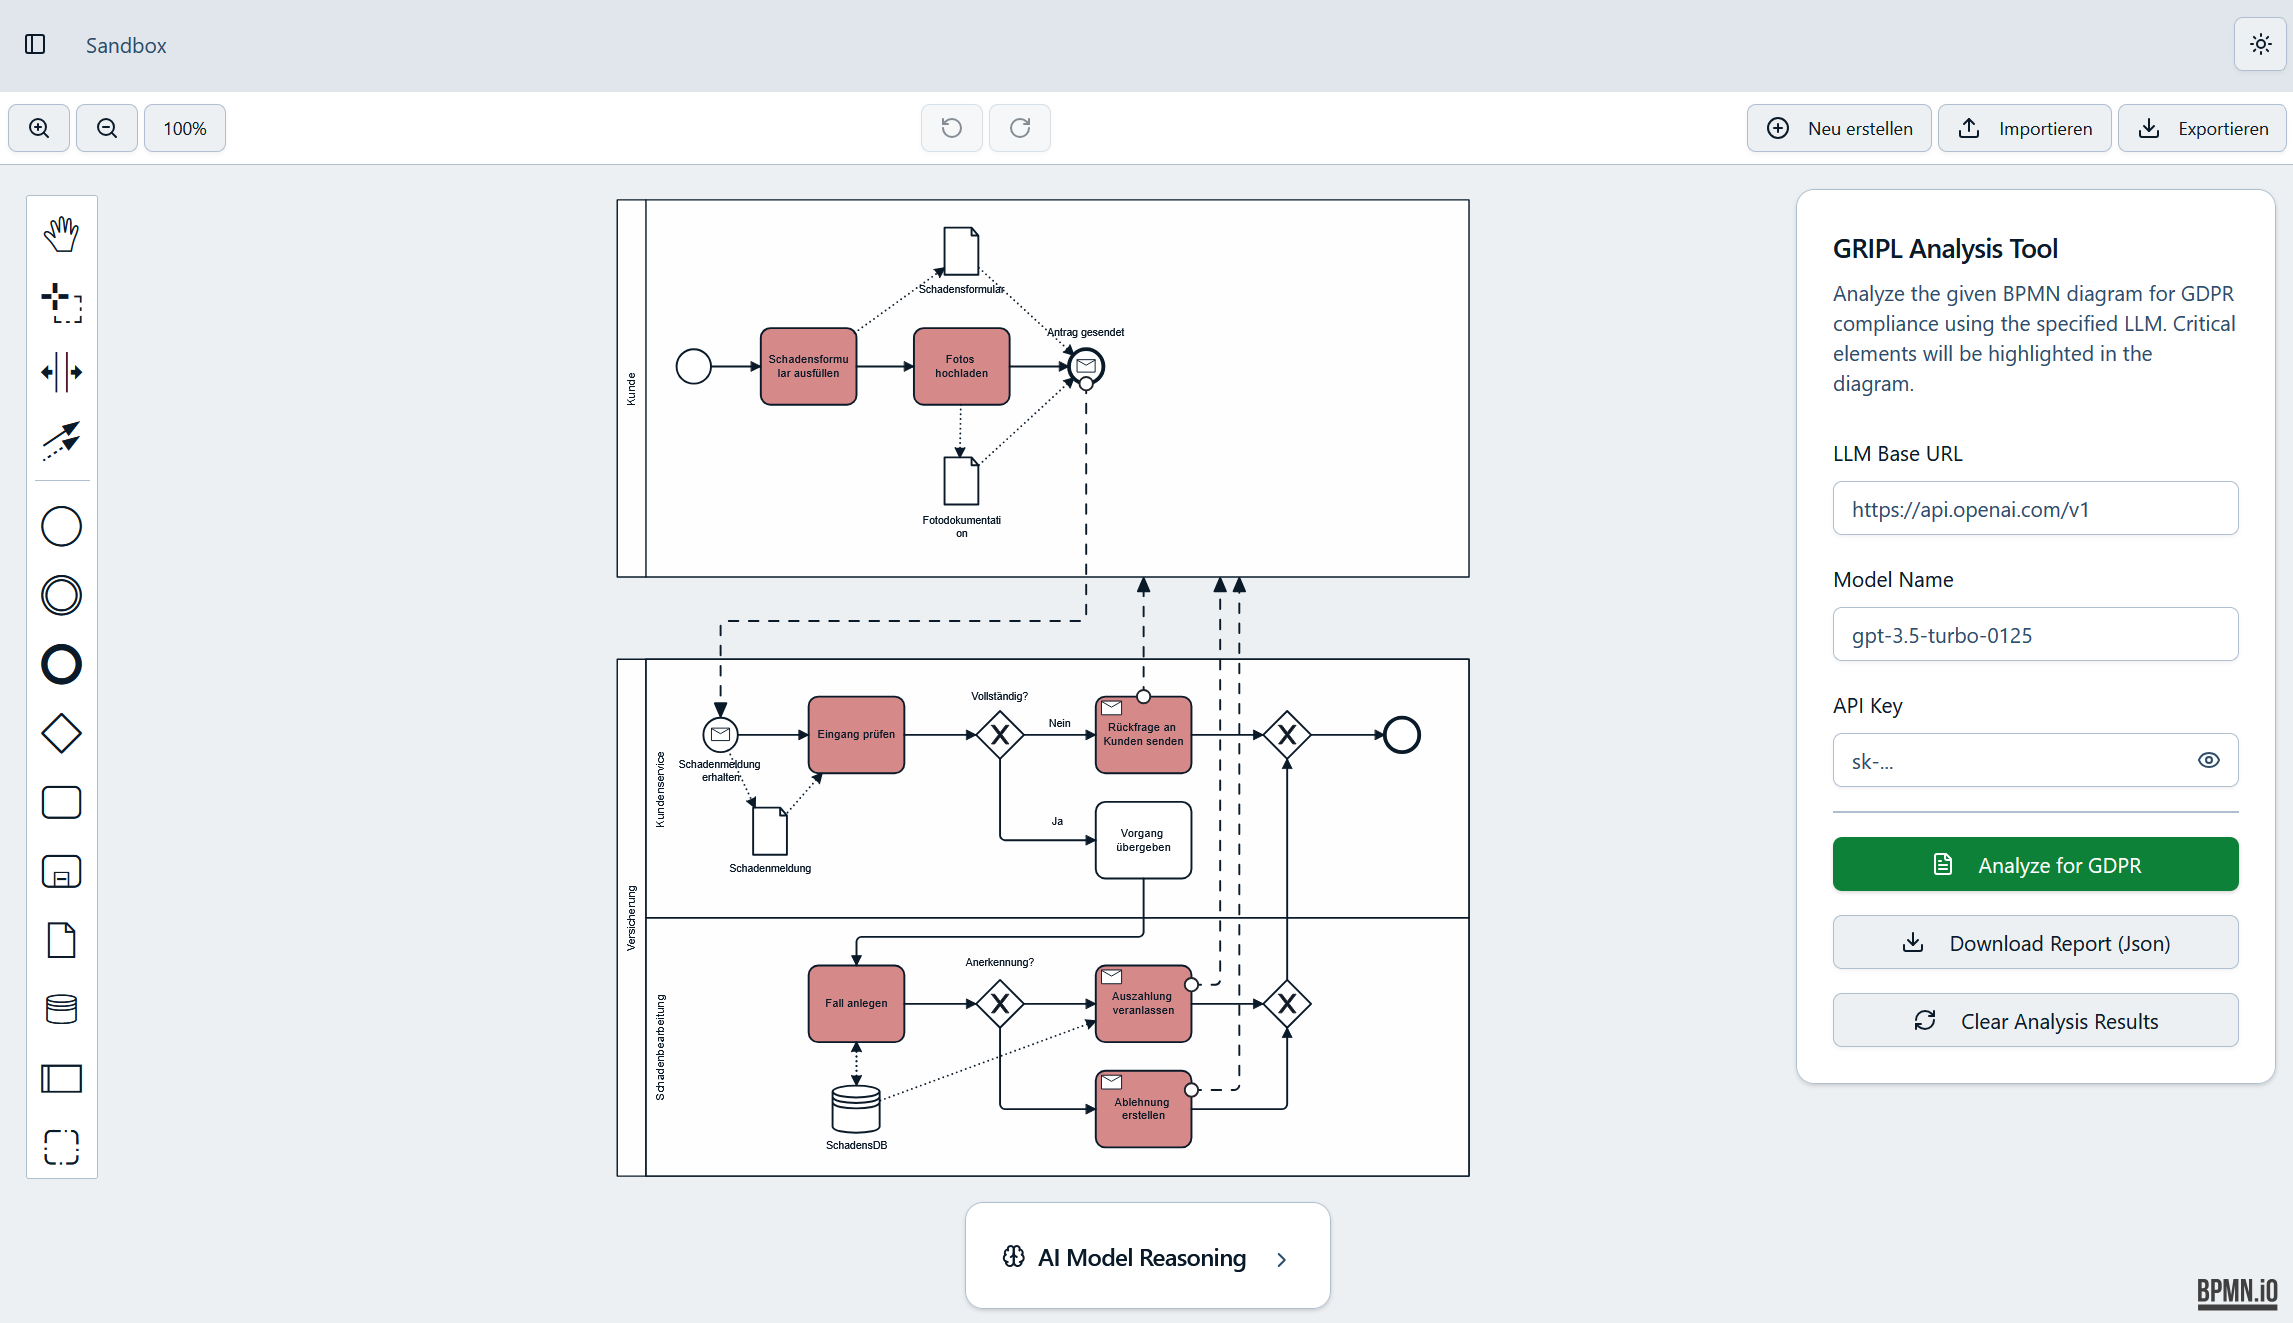
\includegraphics[width=\linewidth]{images/sandbox/sandbox-analyzed-model}
    \caption{Sandbox im Frontend mit hervorgehobenen kritischen Aktivitäten nach Analyse.}
    \label{fig:sandbox-frontend-analyzed-model}
\end{figure}

Außerdem können die vom \ac{LLM} generierten Begründungen zu jeder als kritisch erkannten Aktivität im Editor eingesehen werden. Diese Erläuterungen werden gesammelt in einer aufklappbaren Karte im unteren Bereich des Editors angezeigt, siehe Abbildung \ref{fig:sandbox-frontend-ai-reasoning}.

\begin{figure}
    \centering
    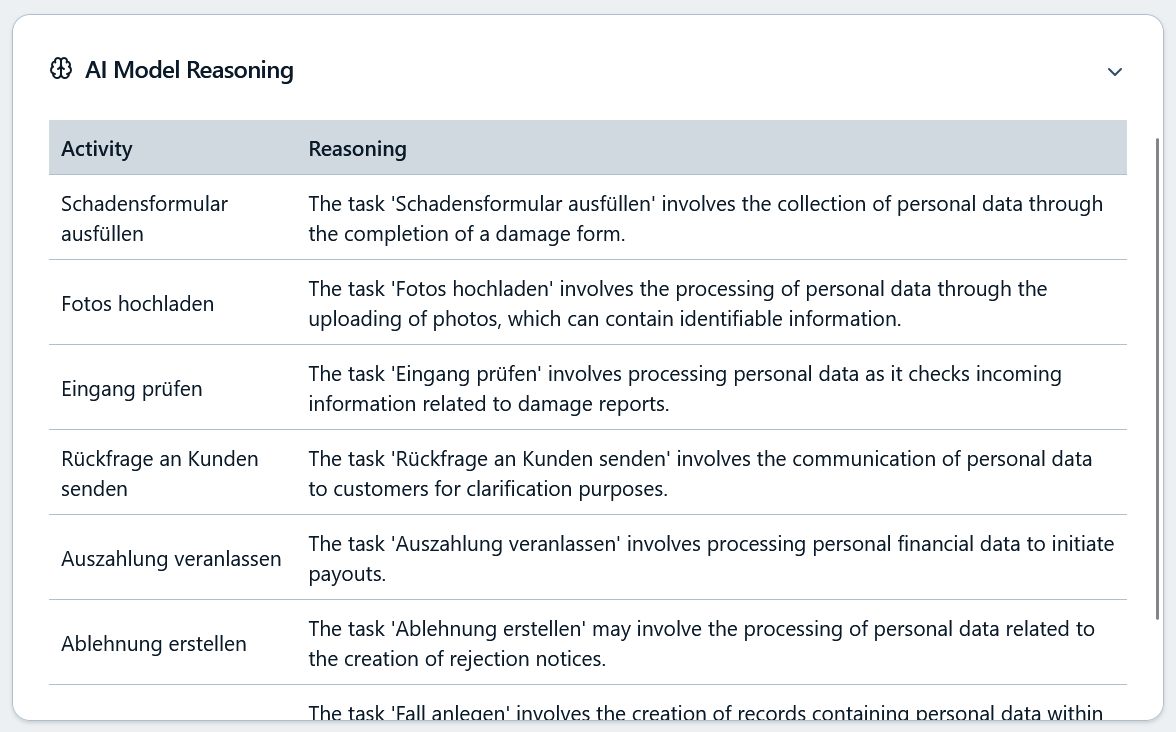
\includegraphics[width=\linewidth]{images/sandbox/sandbox-ai-reasoning}
    \caption{Begründung der Klassifikation durch das LLM in der Sandbox.}
    \label{fig:sandbox-frontend-ai-reasoning}
\end{figure}

Um verschiedene \acp{LLM} vergleichen zu können, verfügt die Sandbox auf der rechten Seite über ein Einstellungsmenü mit konfigurierbaren \ac{LLM}-Parametern (siehe Abbildung \ref{fig:sandbox-frontend-analyzed-model}). Diese Parameter sind identisch zu den in Kapitel \ref{sec:api-design} beschriebenen \texttt{llmProps} und werden beim Starten der Analyse in die API-Anfrage überführt.


\chapter{Labeling und Datensätze}\label{ch:labeling-und-datensatze}

Sowas in die Richtung als Einleitung: Nachdem die Klassifizierung thematisiert worden ist und bevor eine Evaluation der Klassifizierung möglich ist, wie sie im nächsten Kapitel \ref{ch:evaluationsframework}
 thematisiert wird, braucht es gelabelte Testdatensätze mit Testfällen für die Klassifizierung...

Irgendwo muss auch noch definiert werden, dass ein Datensatz aus mehreren Testfällen besteht.

\section{Labeling Tool}\label{sec:labeling-tool}

Um die Erstellung und Verwaltung von gelabelten \ac{BPMN}-Prozessmodellen zu erleichtern, wurde eine Webapp entwickelt. Mit dieser können \ac{BPMN}-Testfälle erstellt, bearbeitet und Aktivitäten mit Labeln versehen werden. Wichtige Funktionen des Labeling-Tools sind dabei: (1) das Anlegen und Verwalten von Datensätzen, (2) die Erstellung beliebig vieler Testfälle pro Datensatz, (3) die direkte Bearbeitung von \ac{BPMN}-Modellen im Browser mittels BPMN.io \cite{bpmnio}, (4) ein Labeling-Modus, in dem Aktivitäten als \ac{DSGVO}-kritisch markiert und optional mit einer Begründung versehen werden können, sowie (5) die persistente Speicherung der annotierten Testfälle in einer Datenbank zur späteren Nutzung im Evaluationsframework (siehe Kapitel~\ref{ch:evaluationsframework}).

Abbildung \ref{fig:labeling-editor} zeigt den Labeling-Editor im Labeling-Modus. Die in der Abbildung nummerierten Bereiche strukturieren die Oberfläche und das Zusammenspiel der Funktionen:

\begin{figure}[h]
    \centering
    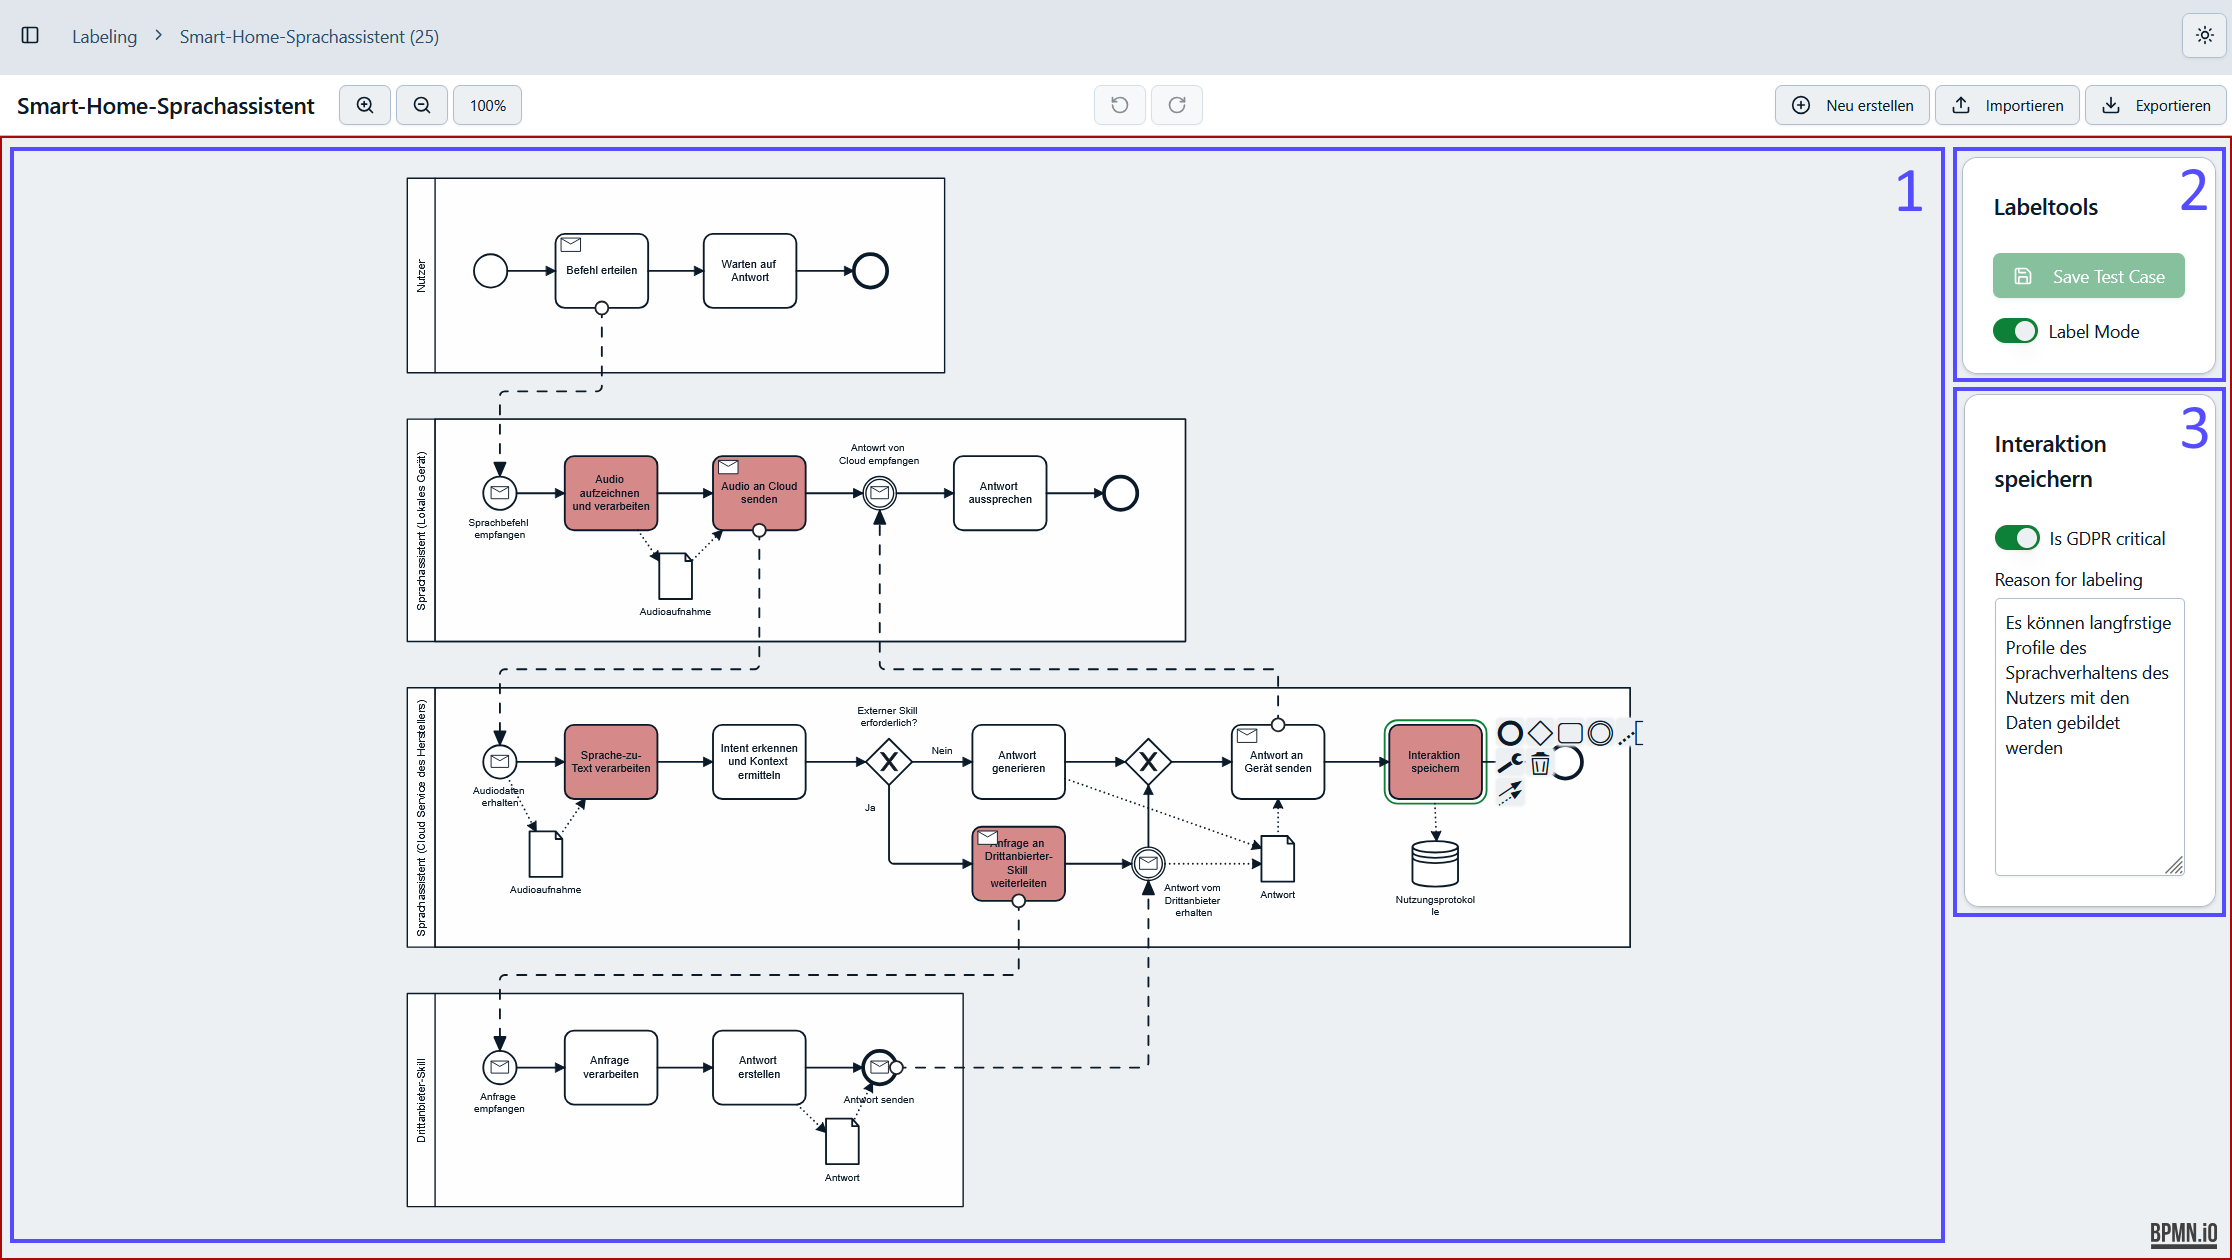
\includegraphics[width=\textwidth]{images/labeling/labeling-editor-annotated}
    \caption{Labeling-Editor im Labeling-Modus mit exemplarischem Modell.}
    \label{fig:labeling-editor}
\end{figure}

\begin{enumerate}
    \item \textbf{BPMN-Editor} (linke Hauptfläche): Hier werden Prozessmodelle erstellt, importiert, bearbeitet und angezeigt. Im Labeling-Modus ist die Modellierung bewusst gesperrt. Die Elemente können dann nur ausgewählt werden, um sie zu labeln. Als kritisch gelabelte Aktivitäten werden im Modell farblich hervorgehoben und sind damit sofort visuell erkennbar.
    \item \textbf{Label-Tools} (rechte Seitenleiste oben): Über dieses Panel wird zwischen Editier- und Labeling-Modus gewechselt und ein Testfall gespeichert.
    \item \textbf{Label-Panel der Aktivität} (rechte Seitenleiste unten): Ist eine Aktivität ausgewählt, kann sie hier als \enquote{DSGVO-kritisch} markiert werden. Zusätzlich lässt sich optional eine natürlichsprachige Begründung hinterlegen. Diese Begründung dient ausschließlich der Dokumentation und Nachvollziehbarkeit und wird nicht in der Evaluierung berücksichtigt.
\end{enumerate}

In der Übersicht der Datensätze aus Abbildung \ref{fig:labeling-datasets} sind alle angelegten Datensätze und zugehörigen Testfälle aufgelistet. Von hier aus können neue Datensätze und Testfälle erstellt sowie bestehende bearbeitet werden.

\begin{figure}[h]
    \centering
    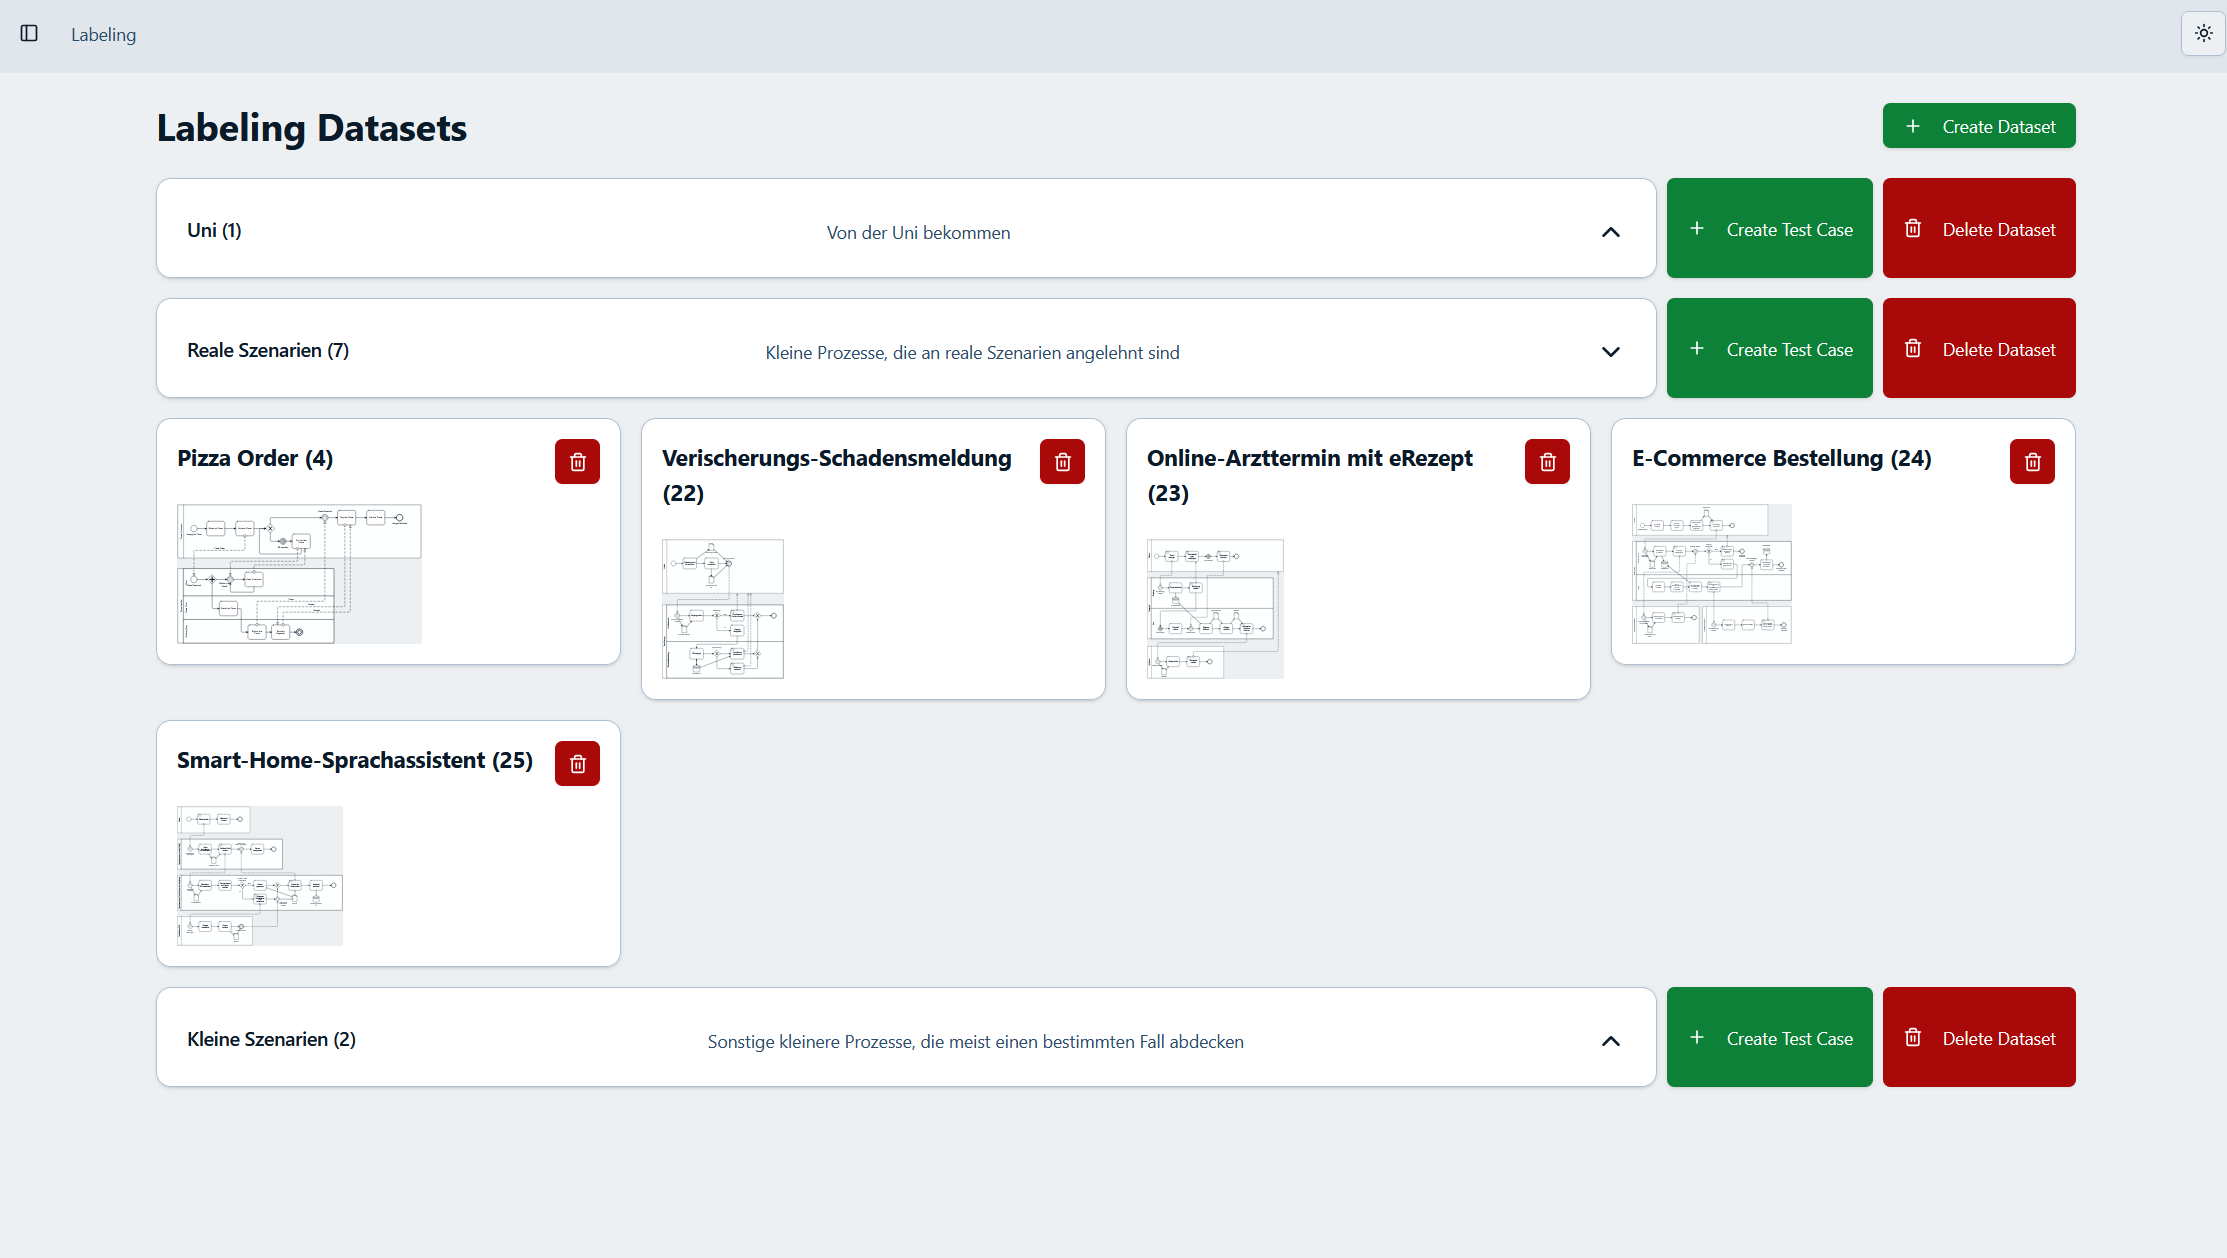
\includegraphics[width=\textwidth]{images/labeling/labeling-datasets}
    \caption{Übersicht der Datensätze im Labeling-Tool.}
    \label{fig:labeling-datasets}
\end{figure}
\section{Quellen und Eigenschaften der Datensätze}\label{sec:quellen-und-eigenschaften-der-datensatze}

Für die Evaluation wurden drei Gruppen von \ac{BPMN}-Datensätzen eingesetzt:

\begin{enumerate}
    \item Prozesse, die von der Universität Ulm bereitgestellt wurden (z.B.\ Lehrbeispiele aus Übungsaufgaben).
    \item Mittelgroße Praxisbeispiele aus verschiedenen Domänen. Diese Prozesse beinhalten Elemente wie Pools, Lanes, Datenobjekte und Gateways.
    \item Kleine, reduzierte Testfälle mit maximal fünf Aktivitäten und wenigen weiteren Elementen (z.\,B. einfacher Sequenzfluss ohne Pools).
\end{enumerate}

Die Praxisbeispiele (Gruppe\,2) decken typische \emph{geschäftliche Domänen} ab, darunter kundenorientierte Service- und Bestellprozesse (E-Commerce), fachliche Abläufe im Versicherungs- und Gesundheitswesen sowie technische Smart-Home/IoT-Kontexte. Die universitären Beispiele (Gruppe~1) stammen aus lehrnahen Übungsaufgaben und stellen Domänen wie wie Finanzen, Logistik und HR dar. Die kleinen Testfälle (Gruppe\,3) sind bewusst minimal gehalten, um Randfälle und unterschiedliche Modellkomplexitäten abzudecken.

Diese bewusst heterogene Auswahl über Domänen, Sprachen und Komplexitätsstufen erhöht die Aussagekraft der Evaluation. In der Literatur wird betont, dass eine erhöhte Datensatzvielfalt die Robustheit der Bewertung steigert und einseitige Ergebnisse vermeidet \cite{blake2025datasetdiversity}. Tabelle \ref{tab:datensaetze-eckdaten} zeigt die Eckdaten der Datensätze.

\begin{table}[htbp]
    \centering
    \begin{threeparttable}
    \caption{Eckdaten der verwendeten Datensätze}
    \label{tab:datensaetze-eckdaten}
    \begin{tabular}{l r r r}
        \toprule
        & Uni-Prozesse & Reale Szenarien & Kleine Testfälle \\
        \midrule
        Testfälle Gesamt                  & 5  & 5 & 14 \\
        Testfälle (DE)                    & 0 & 3 & 15 \\
        Testfälle (EN)                    & 5 & 2 & 0 \\
        Ø Aktivitäten $\pm$ SD\tnote{1}   & 13,4 $\pm$ 2,6 & 11,6 $\pm$ 4,2 & 3,9 $\pm$ 1,4 \\
        Ø Aktivitäten (kritisch) $\pm$ SD & 8,6 $\pm$ 3,6 & 6,6 $\pm$ 1,9 & 2,1 $\pm$ 1,5 \\
        Ø Datenobjekte $\pm$ SD           & 1,4 $\pm$ 1,9 & 3,6 $\pm$ 2,1 & 0,4 $\pm$ 0,7 \\
        Ø Datenassoziationen $\pm$ SD     & 2,4 $\pm$ 3,3 & 7 $\pm$ 4 & 0,7 $\pm$ 1,2 \\
        Ø Ereignisse $\pm$ SD             & 21 $\pm$ 13,8 & 8,2 $\pm$ 2,8 & 2 $\pm$ 0 \\
        Ø Gateways $\pm$ SD               & 13 $\pm$ 7,6 & 1,8 $\pm$ 1,5 & 0 $\pm$ 0 \\
        Ø Pools $\pm$ SD                  & 3,4 $\pm$ 1,1 & 3 $\pm$ 1 & 0,4 $\pm$ 0,6 \\
        Ø Lanes $\pm$ SD\tnote{2}         & 3 $\pm$ 1 & 4 $\pm$ 0,7 & 0,3 $\pm$ 0,5 \\
        Ø Nachrichtenflüsse $\pm$ SD      & 9,4 $\pm$ 5,3 & 5,2 $\pm$ 0,8 & 0,1 $\pm$ 0,3 \\
        Ø Annotationen $\pm$ SD           & 1 $\pm$ 1,7 & 0 $\pm$ 0 & 0 $\pm$ 0 \\
        \bottomrule
    \end{tabular}
    \begin{tablenotes}
        \item[1] SD = Standardabweichung $s$ der jeweiligen Anzahl pro Testfall.
        \item[2] Blackbox-Pools ohne Lanes wurden nicht mitgezählt, daher kann der Durchschnittswert der Lanes geringer ausfallen als der, der Pools.
    \end{tablenotes}
    \end{threeparttable}
\end{table}
\section{Labeling-Guide}\label{sec:labeling-guide}

Die Aktivitäten in den Testfällen sollen mit dem Label \enquote{kritisch} versehen werden, wenn sie potenziell personenbezogene Daten verarbeiten und somit im Sinne der \ac{DSGVO} relevant sein könnten. Die wichtigsten Begriffe der \ac{DSGVO} wurden bereits in Abschnitt \ref{sec:dsgvo} definiert.

Beim Labeln einer Aktivität können Grenzfälle auftreten, insbesondere wenn kein Datenobjekt vorhanden ist, der Name einer Aktivität aber auf Datenverarbeitung hinweist, wie z.\,B. \enquote{Verträge archivieren}. Dabei kann es sich sowohl um personenbezogene Verträge, wie Arbeitsverträge, als auch um rein geschäftliche Verträge zwischen Unternehmen handeln. In einem solchen Fall wird zuerst geschaut, ob der Kontext der Aktivität Hinweise auf personenbezogene Daten gibt (z.\,B. Pool/Lane oder andere Aktivitäten im Prozess). Wenn keine eindeutigen Hinweise vorliegen, wird die Aktivität als unkritisch gelabelt. Wenn jedoch der Kontext auf die Verarbeitung personenbezogener Daten hinweist (z.\,B. ein Prozessname wie \enquote{Mitarbeiterverwaltung} oder vorherigere Aktivitäten wie \enquote{Mitarbeiterdaten erfassen}), wird die Aktivität als kritisch gelabelt. Im Zweifel wird die Aktivität als kritisch gelabelt, um eine höhere Sensitivität zu gewährleisten.

Tabelle \ref{tab:labeling-examples} listet beispielhaft einige Aktivitäten mit ihrer Klassifikation und einer Begründung auf.

\begin{table}[htbp]
    \centering
    \caption{Beispielhafte Aktivitäten und Label}
    \begin{tabularx}{\textwidth}{p{0.4\textwidth} c p{0.4\textwidth}}
        \toprule
        Aktivität & Kritisch? & Kommentar \\
        \midrule
        Lieferadresse eingeben & Ja & Name, Anschrift des Kunden werden aufgenommen. \\
        Rückfrage an Kunden senden & Ja & Kontaktinformationen werden verwendet. \\
        Fall anlegen & Ja & Aktivität befindet sich im Kundenservice-Kontext, personenbezogene Daten wahrscheinlich. \\
        Sprache zu Text verarbeiten & Ja & Im Kontext eines Sprachassistenten werden biometrische Daten des nutzers verarbeitet. \\
        Produkt versenden & Nein^* & Logistik und Sachvorgänge sind nicht per se Datenschutzkritisch, solange keine neue Datenverarbeitung, wie ein Labeldruck stattfindet. \\
        Systemprotokoll auslesen & Ja & Im Kontext einer technischen Wartung können personenbezogene Daten (z.\,B. Nutzer-\texttt{ids}) enthalten sein. \\
        Logdaten archivieren (anonym) & Nein & Keine personenbezogenen Daten enthalten. \\
        Gerät kalibrieren & Nein & Im Kontext einer technischen Wartung werden keine personenbezogenen Daten verarbeitet. \\
        \bottomrule
    \end{tabularx}
    \label{tab:labeling-examples}
\end{table}
% Functional-Requirement Table Design
%
% Oberhalb und unterhalb des Zeilen Contents muss noch irgendwie Platzeingefügt werden
\newcounter{linkcount}
\newcounter{linktotal}

\newcommand{\countLinks}[1]{%
    \setcounter{linkcount}{0}%
    \setcounter{linktotal}{0}%
    \renewcommand*{\do}[1]{\stepcounter{linktotal}}%
    \docsvlist{#1}%
}

\newcommand{\createHyperlinks}[1]{%
    \ifthenelse{\equal{#1}{-}}%
    {-}%
    {%
        \countLinks{#1}%
        \renewcommand*{\do}[1]{%
            \stepcounter{linkcount}%
            \hyperlink{FA##1}{FA##1}%
            \ifnum\value{linkcount}<\value{linktotal}%
            ,\ %
            \fi%
        }%
        \docsvlist{#1}%
    }%
}

\newcommand{\reqTable}[4]{
        {\rowcolors{2}{gray!50!white!20}{gray!40!white!10}
    \phantomsection\hypertarget{FA#1}{}
    \begin{tabular}{ p{3cm} p{10.2cm} }
        \rowcolor{darkgray}\textcolor{white}{\textbf{ID:}} & \textcolor{white}{\textbf{FA#1}} \\
        Titel: & #2 \\
        Beschreibung: & #3 \\
        Abhängigkeit: & \createHyperlinks{#4} \\
    \end{tabular}
    }
}

\newcommand{\createHyperlinksNFA}[1]{%
    \ifthenelse{\equal{#1}{-}}%
    {-}%
    {%
        \countLinks{#1}%
        \renewcommand*{\do}[1]{%
            \stepcounter{linkcount}%
            \hyperlink{NFA##1}{NFA##1}%
            \ifnum\value{linkcount}<\value{linktotal}%
            ,\ %
            \fi%
        }%
        \docsvlist{#1}%
    }%
}
\chapter{Evaluationsframework}\label{ch:evaluationsframework}

Nachdem nun Daten gelabelt werden können und der Testdatensatz für diese Arbeit erstellt wurde, wird in diesem Kapitel das Evaluationsframework vorgestellt. Das Framework nutzt die in Kapitel~\ref{ch:klassifizierungsalgorithmus-(design-und-implementierung)} entwickelte Klassifizierungspipeline, um verschiedene \acp{LLM} anhand gelabelter Testdaten systematisch, reproduzierbar und transparent zu vergleichen. Leitendes Gestaltungsprinzip ist die Entkopplung: Modelle, Klassifizierungsendpunkte und Testdaten werden zur Laufzeit über eine deklarative Konfiguration und eine standardisierte HTTP-Schnittstelle, siehe Abschnitt~\ref{sec:api-design}, angebunden. Dadurch sind sie austauschbar und erweiterbar, ohne Codeänderungen vornehmen zu müssen, zum Beispiel durch die Einbindung eines neuen Modells mit Endpunkt, Modellname und Parametern wie \emph{temperature} oder \emph{topP} sowie durch zusätzliche Datensätze. So wird ein fairer und reproduzierbarer Vergleich unterschiedlicher Modelle unter identischen Rahmenbedingungen ermöglicht.

\section{Use-Cases und Anforderungen}\label{sec:anforderungen-und-use-cases}

Das Evaluationsframework richtet sich an Forschende und Entwickler, die \acp{LLM} und Klassifizierungsalgorithmen für die Identifikation \ac{DSGVO}-kritischer \ac{BPMN}-Aktivitäten auswerten und miteinander vergleichen möchten. Es bietet eine einheitliche Ausführungs- und Auswertungsumgebung mit klar definierten Schnittstellen und standardisierten Berichten. In diesem Kapitel werden die Use-Cases udn Anforderungen des Evaluationsframeworks beschrieben.

\subsection*{Use-Cases}

Die wichtigsten Anwendungsfälle des Evaluationsframeworks sind:

\begin{itemize}
    \item \textbf{Benchmarking von LLMs.} Systematischer Vergleich mehrerer \acp{LLM} auf denselben Datensätzen, mit identischem Algorithmus und identischen Parametern.
    \item \textbf{A/B-Vergleich von Algorithmen.} Gegenüberstellung verschiedener Klassifizierungspipelines, mit z.B.\ alternativen Prompts oder anderem Preprocessing, über eine standardisierte HTTP-Schnittstelle, die in Kapitel~\ref{sec:api-design} definiert ist.
    \item \textbf{Explorative Analyse.} Detaillierte Einsicht pro Modell und Testfall (inklusive Begründungen und Visualisierungen), um Fehlklassifikationen gezielt zu untersuchen.
    \item \textbf{Berichterstellung.} Die Ergebnisse lassen sich als JSON oder Markdown exportieren und später wieder importieren, um sie erneut untersuchen zu können. Sie eignen sich zudem für die Publikation. Die Diagramme werden automatisch erzeugt und stehen ebenfalls zum Download bereit.
\end{itemize}

In dieser Arbeit werden keine A/B-Vergleiche unterschiedlicher Klassifizierungsalgorithmen durchgeführt, sondern lediglich verschiedene \acp{LLM} mit demselben Algorithmus verglichen. Das Framework ist jedoch so konzipiert, dass dies in zukünftigen Arbeiten möglich ist.

\subsection*{Funktionale Anforderungen}

In der folgenden Tabelle sind die funktionalen Anforderungen an das Evaluationsframework aufgelistet, die notwendig sind um Use-Cases zu erfüllen:

\begin{center}
    \reqTable{01}
    {Nutzen gelabelter Testdatensätze}
    {Das Framework kann die gelabelten Testdatensätze benutzten, die mit dem Labeling-Tool aus \ref{sec:labeling-tool} erstellt worden sind.}
    {}
\end{center}

\begin{center}
    \reqTable{02}
    {Vergleichbarkeit von Modellen und Algorithmen}
    {Das Framework erlaubt den direkten Vergleich verschiedener \acp{LLM} sowie unterschiedlicher Klassifizierungsalgorithmen anhand gelabelter Testdaten. Die Anbindung an Klassifizierungsalgorithmen erfolgt über die in Kapitel~\ref{sec:api-design} definierte, standardisierte HTTP-Schnitstelle.}
    {01}
\end{center}

\begin{center}
    \reqTable{03}
    {Deklarative Konfiguration}
    {Ein Evaluationslauf ist vollständig über eine YAML-Datei konfigurierbar. Dazu zöhlen Modelle, Klassifizierungsendpunkte, Testdatensätze, Seed. Experimente werden dadurch portabel und wiederholbar.}
    {02}
\end{center}

\begin{center}
    \reqTable{04}
    {Detaillierte Ergebnisaufbereitung}
    {
    Das Framework gibt Ergebnisse auf zwei Ebenen aus.
    \begin{enumerate}
        \item Pro Testfall und pro Modell: Status (\enquote{bestanden}/\enquote{nicht bestanden}), klassifizierte Elemente mit Begründungen, \ac{TP}/\ac{FP}/\ac{FN}/\ac{TN} und eine Visualisierung der Klassifikation im \ac{BPMN}-Prozess.
        \item Pro Modell als Summe über alle Testfälle: Accuracy, Precision, Recall, F1-Score und die Konfusionsmatrix.
    \end{enumerate}
    Zusätzlich protokolliert das Framework Metadaten der Evaluation, z.\,B. Endpunkt, verwendete Modelle und den Seed.
    }
    {02}
\end{center}

\begin{center}
    \reqTable{05}
    {Frontend}
    {Für eine einfache Bedienung und Ansicht der Ergebnisse bietet das Evaluationsframework ein Frontend an.}
    {02,03,04}
\end{center}

\begin{center}
    \reqTable{06}
    {Visualisierung und Berichte der Gesamtresultate}
    {Kennzahlen werden als Side-by-Side-Diagramme und tabellarisch dargestellt. Zusätzlich stehen Export/Import der Ergebnisse als JSON sowie ein Markdown-Report zur Verfügung.}
    {05}
\end{center}
\section{Konfiguration einer Evaluierung}\label{sec:konfiguration-einer-evaluierung}

Die funktionale Anforderung \hyperlink{FA03}{FA03} fordert, dass Evaluationsläufe deklarativ konfiguriert werden können. Das Framework unterstützt dies auf zwei Wegen:
Erstens bietet die Weboberfläche, die in \ref{sec:visualisierung-im-frontend} gezeigt wird, die Möglichkeit, Evaluationsläufe interaktiv zu konfigurieren und zu starten.
Zweitens lässt sich eine Evaluierung über eine YAML-Datei beschreiben, die entweder in der Weboberfläche hochgeladen oder per CLI an das Evaluationsframework übergeben wird. Auf diese Weise werden Reproduzierbarkeit und Versionierung der Evaluationsläufe sichergestellt. Listing \ref{lst:evaluation-config} zeigt ein Beispiel für eine solche YAML-Konfiguration. Ein ausführliches JSON-Schema ist im Anhang (Listing \ref{lst:evaluation-config-schema}) zu finden.

Die Evaluierungskonfiguration umfasst die folgenden Bausteine:

\begin{itemize}
    \item \texttt{defaultEvaluationEndpoint} ist der Standardendpunkt für die Klassifizierung. Er wird verwendet, wenn für ein Modell kein eigener Endpunkt angegeben ist. Der Endpunkt muss die in Kapitel \ref{sec:api-design} beschriebene API-Spezifikation erfüllen und kann relativ (gegen die Basis-URL des Evaluationsframeworks) oder absolut (für einen externen Dienst) angegeben werden.
\end{itemize}

\begin{lstlisting}[caption={Beispiel einer Evaluierungskonfiguration in YAML.},label={lst:evaluation-config}]
defaultEvaluationEndpoint: /gdpr/analysis/prompt-engineering
maxConcurrent: 10
repetitions: 3
seed: 42
models:
  - label: Mistral Medium 3.1
    llmProps:
      baseUrl: https://openrouter.ai/api/v1
      modelName: mistralai/mistral-medium-3.1
      apiKey: ${OPEN_ROUTER_API_KEY}
      topP: 1
  - label: Deepseek Chat v3.1
    llmProps:
      baseUrl: https://openrouter.ai/api/v1
      modelName: deepseek/deepseek-chat-v3.1
      apiKey: ${OPEN_ROUTER_API_KEY}
      temperature: 0.1
  - label: GPT oss 120b
    llmProps:
      baseUrl: https://openrouter.ai/api/v1
      modelName: openai/gpt-oss-120b
      apiKey: ${OPEN_ROUTER_API_KEY}
datasets:
  - 2
  - 7
\end{lstlisting}

\begin{itemize}
    \item \texttt{maxConcurrent} gibt die maximale Anzahl parallel auszuführender Testfälle an. So lassen sich beispielsweise \emph{Rate Limits}\footnote{Providerseitige Begrenzungen, etwa \enquote{Requests pro Minute} oder maximale Parallelität. Bei Überschreitung antworten viele Anbieter mit HTTP~429 (\enquote{Too Many Requests}). Zudem drohen strengere Drosselungen.} der angebundenen \acp{LLM} einhalten, um technische Fehler in den Ergebnissen zu vermeiden.
    \item \texttt{repetitions} bestimmt, wie oft die Evaluierung pro Modell wiederholt wird. Die Ergebnisse werden später über alle Wiederholungen aggregiert (siehe Abschnitt~\ref{sec:generierte-resultate}).
    \item \texttt{seed} legt einen Startwert (Seed) für reproduzierbare Evaluationsläufe fest. Auf Basis des Seeds und der Wiederholungsnummer wird für jede Wiederholung deterministisch ein eigener Seed generiert, um unterschiedliche, aber reproduzierbare Ergebnisse zu erzielen. Er wird bei jedem Modell an die \texttt{llmProps} weitergereicht und bei der Kommunikation mit den \acp{LLM} verwendet, sofern diese einen Seed unterstützen.
    \item \texttt{models} enthält die zu evaluierenden Modelle. Jedes Modell besitzt ein \texttt{label} zur Identifikation und optional spezifische \texttt{llmProps}, um die Eigenschaften des verwendeten \acp{LLM} zu definieren. Diese sind identisch zu den in Kapitel \ref{sec:api-design} beschriebenen \texttt{llmProps}.
    \item \texttt{datasets} ist eine Liste von Datensatz-\texttt{ids}, die jeweils eine Menge von Testfällen beinhalten.
\end{itemize}

Wie im Schema in Listing \ref{lst:evaluation-config-schema} gezeigt, kann jedem Modell optional ein eigener\linebreak~\texttt{evaluationEndpoint} zugewiesen werden, der den in \texttt{defaultEvaluation-\linebreak~Endpoint} definierten Standard überschreibt. Dadurch lassen sich unterschiedliche Klassifizierungsalgorithmen oder -versionen gezielt pro Modell vergleichen. Ist kein spezifischer Endpunkt angegeben, greift automatisch der Standardendpunkt.

API-Keys in den \texttt{llmProps} können optional als Umgebungsvariablen referenziert werden, wie im Beispiel in Listing \ref{lst:evaluation-config} gezeigt. So lassen sich sensible Daten sicher handhaben, ohne sie direkt in der Konfigurationsdatei zu speichern. Die Umgebungsvariablen werden zur Laufzeit aufgelöst und müssen daher im Kontext der Anwendung verfügbar sein.
\section{Architektur und Komponenten}\label{sec:architektur-und-komponenten}

\begin{itemize}
    \item Diagramm zur Architektur erstellen
    \item HTTP-Endpunkt oder CLI zum Starten -> Holen der notwendigen Testdatensätze -> Aufruf der Klassifizierung pro Modell und pro Testcase -> Akkumulieren der Ergebnisse pro Testcase + ggf. frühzeitige Rückgabe des Ergebnisses des Testcase für Live-Ansicht in UI -> Aufarbeiten der akkumulierten Ergebnisse und berechnen wichtiger Metriken
    \item EvaluationController, MultiEvaluationRunner, EvaluationRunner, HttpEvaluator, MetricsAccumulator, ggf. Frontend (Concurrency von MultiEvaluationRunner)
\end{itemize}

\section{Evaluationsergebnisse}\label{sec:generierte-resultate}

Die im Folgenden beschriebenen Resultate werden während der Evaluierung laufend erzeugt und an das Frontend gestreamt. Anwender können damit sowohl Zwischenstände verfolgen als auch nach Abschluss detaillierte Analysen durchführen.

Für jeden Testfall eines Modells liegen vor: die von der Klassifizierungspipeline klassifizierten Aktivitäten mit optionalen Begründungen, die gelabelten erwarteten Aktivitäten, die Zählwerte für \emph{\ac{TP}}, \emph{\ac{FP}}, \emph{\ac{FN}} und \emph{\ac{TN}} sowie eine Bild-URL zur Visualisierung des \ac{BPMN}-Modells mit hervorgehobenen Aktivitäten. Aus diesen Informationen lässt sich ableiten, ob der Testfall erfolgreich war. Ein Testfall gilt als erfolgreich, wenn die klassifizierten Aktivitäten exakt den erwarteten Aktivitäten entsprechen. Technische Probleme, die während der Klassifizierung auftreten, werden ebenfalls erfasst, z.\,B.\ Parsing-Fehler, ungültiges \ac{BPMN}, Token-Limit-Überschreitungen oder Zeitüberschreitungen.

Auf Modellebene stehen die Gesamtergebnisse über alle Testfälle zur Verfügung. Dazu gehören die aggregierten Kennzahlen \emph{Precision}, \emph{Accuracy}, \emph{Recall} und \emph{F1-Score} sowie eine Konfusionsmatrix mit den Gesamtwerten für \emph{\ac{TP}}, \emph{\ac{FP}}, \emph{\ac{FN}} und \emph{\ac{TN}}. Zusätzlich sind die Anzahlen der korrekt bzw.\ falsch klassifizierten sowie der technisch fehlgeschlagenen Testfälle aufgeführt.

Die Ergebnisse eines Modells über alle Testfälle werden zudem auch über alle Wiederholungen aggregiert. Das Framework berechnet pro Kennzahl den Mittelwert und die Standardabweichung. Dadurch lassen sich zufallsbedingte Schwankungen abfedern und robustere Aussagen treffen.

Abschließend sind die Metadaten der gesamten Evaluierung verfügbar. Dazu zählen die verwendeten Testdatensätze und Anzahl der Testfälle, die konfigurierten Modelle samt ihrer relevanten Parameter (u.\,a.\ Modellname, \texttt{temperature}, \texttt{top-p}, ggf.\ eigener Endpunkt), der für die Reproduzierbarkeit verwendete Seed sowie ein Zeitstempel der Evaluierung. Zum unmittelbaren Vergleich werden die aggregierten Kennzahlen aller Modelle nebeneinander dargestellt. Alle Ergebnisse können über ein webbasiertes Frontend, das im nächsten Abschnitt beschrieben wird, eingesehen und im Detail analysiert werden.

\section{Nutzung über Webapp}\label{sec:nutzung-uber-webapp}

Zur interaktiven Nutzung der Klassifizierung wurde eine \emph{Sandbox} in Form einer Webapp entwickelt. Sie verbindet einen vollwertigen \ac{BPMN}-Editor auf Basis von \texttt{BPMN.js} \cite{bpmn-js} mit der in Kapitel~\ref{sec:api-design} beschriebenen HTTP-Schnittstelle und macht die Analyse damit ganz einfach bedienbar. In der Sandbox können \ac{BPMN}-Modelle erstellt, verändert, exportiert und importiert sowie auf Datenschutzrelevanz analysiert werden. Als kritisch klassifizierte Aktivitäten werden nach der Analyse direkt im Editor farblich hervorgehoben, wie in Abbildung \ref{fig:sandbox-frontend-analyzed-model} zu sehen.

\begin{figure}
    \centering
    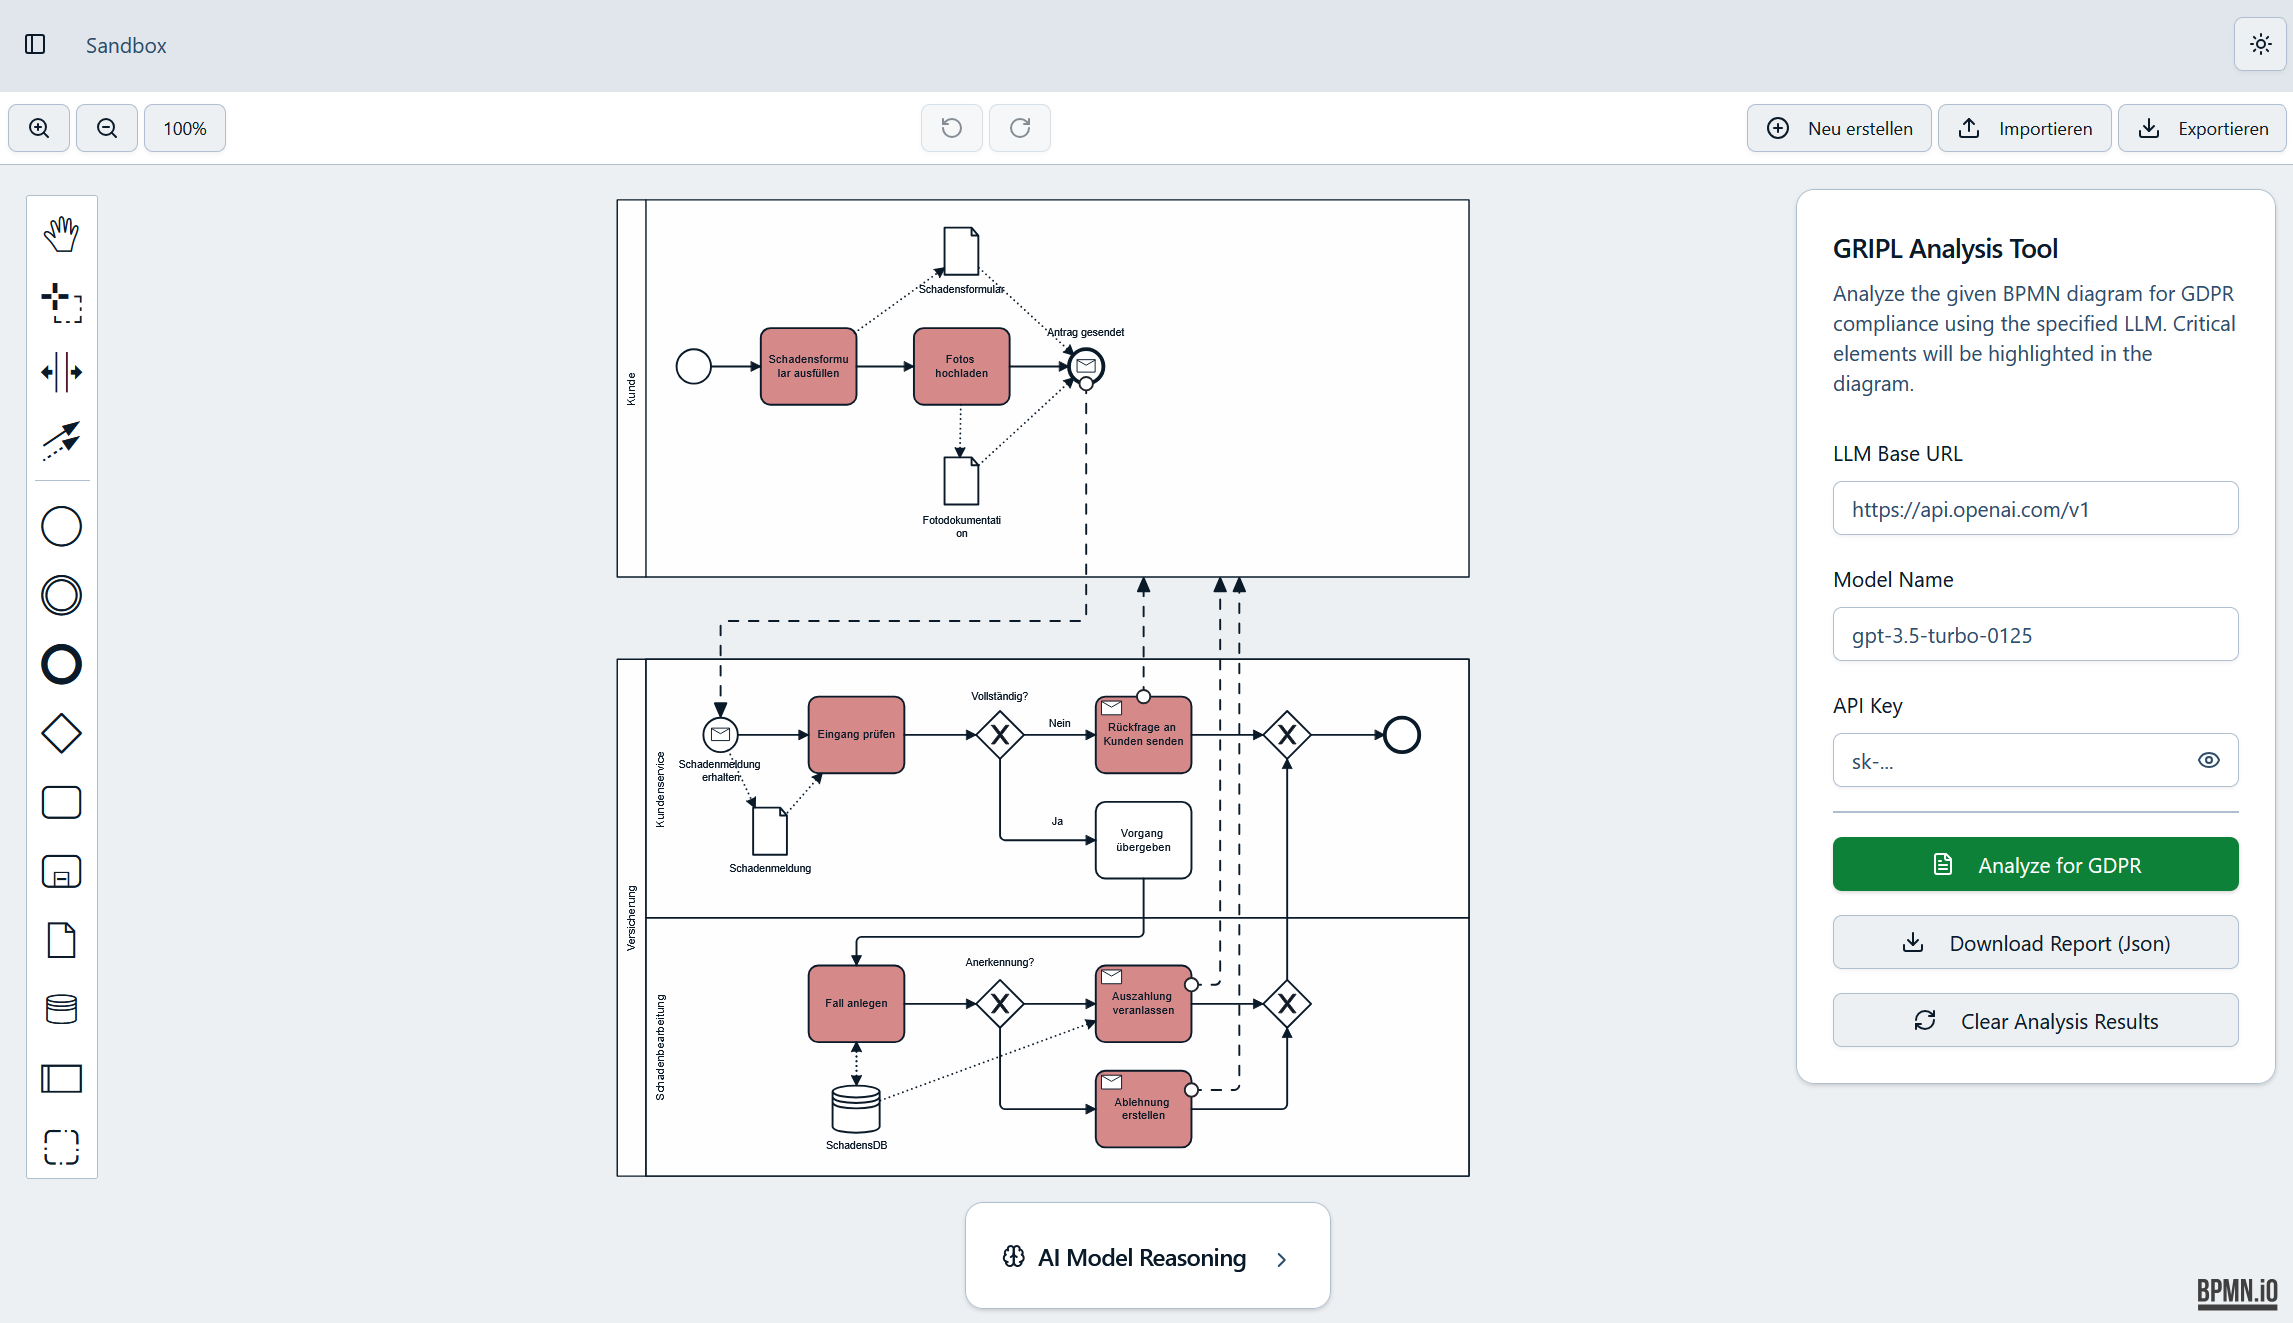
\includegraphics[width=\linewidth]{images/sandbox/sandbox-analyzed-model}
    \caption{Sandbox im Frontend mit hervorgehobenen kritischen Aktivitäten nach Analyse.}
    \label{fig:sandbox-frontend-analyzed-model}
\end{figure}

Außerdem können die vom \ac{LLM} generierten Begründungen zu jeder als kritisch erkannten Aktivität im Editor eingesehen werden. Diese Erläuterungen werden gesammelt in einer aufklappbaren Karte im unteren Bereich des Editors angezeigt, siehe Abbildung \ref{fig:sandbox-frontend-ai-reasoning}.

\begin{figure}
    \centering
    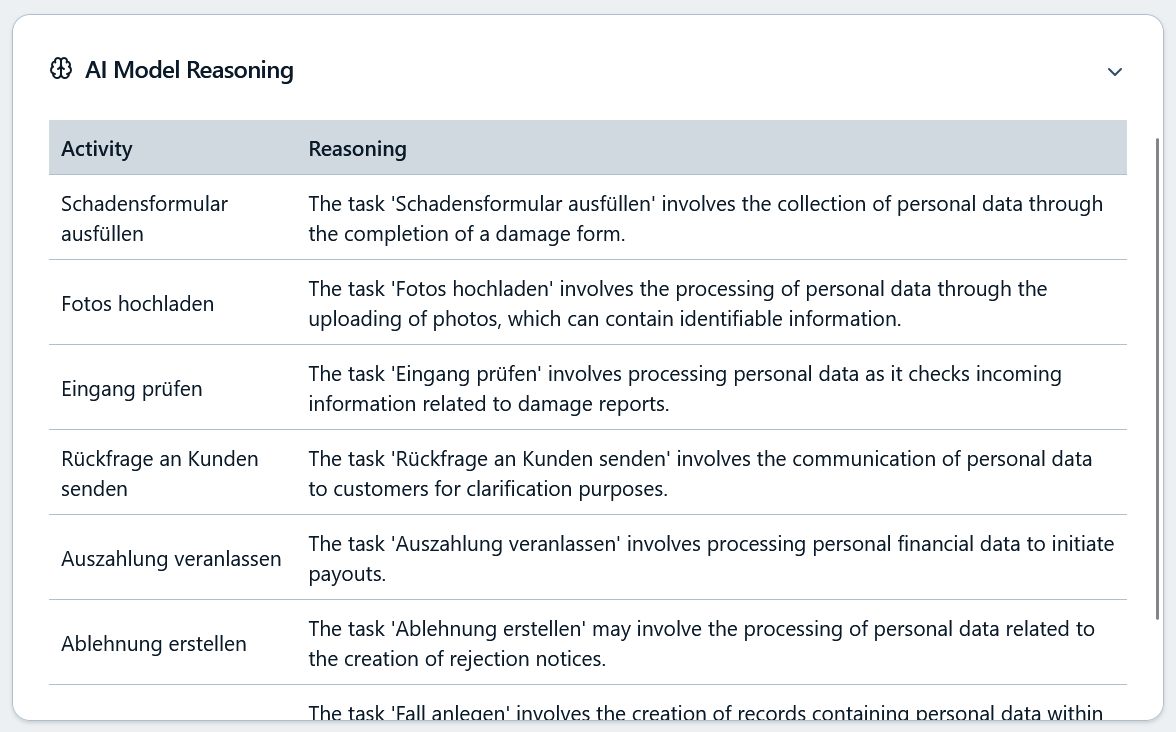
\includegraphics[width=\linewidth]{images/sandbox/sandbox-ai-reasoning}
    \caption{Begründung der Klassifikation durch das LLM in der Sandbox.}
    \label{fig:sandbox-frontend-ai-reasoning}
\end{figure}

Um verschiedene \acp{LLM} vergleichen zu können, verfügt die Sandbox auf der rechten Seite über ein Einstellungsmenü mit konfigurierbaren \ac{LLM}-Parametern (siehe Abbildung \ref{fig:sandbox-frontend-analyzed-model}). Diese Parameter sind identisch zu den in Kapitel \ref{sec:api-design} beschriebenen \texttt{llmProps} und werden beim Starten der Analyse in die API-Anfrage überführt.
\chapter{Modellauswahl}\label{ch:modellauswahl}

\section{Kriterien}\label{sec:kriterien}

Dieser Abschnitt legt die Auswahlkriterien der \acp{LLM} offen. Ziel ist es, die Auswahl nachvollziehbar zu machen und eine Grundlage für zukünftige Arbeiten zu schaffen, die ähnliche Modelle evaluieren möchten.

\subsection*{Einordnung als \ac{EU}-Modell vs. internationales}

Als \enquote{\ac{EU}‑Modell} gelten Modelle, deren Anbieter ihren Hauptsitz in der \ac{EU} haben, deren Veröffentlichung in der \ac{EU} erfolgt oder die schwerpunktmäßig in der \ac{EU} entwickelt oder verfeinert wurden. Alle anderen Modelle werden als \enquote{international} eingeordnet. Diese Klassifizierung hilft, europäische von nicht‑europäischen Modelle zu unterscheiden.

\subsection*{Definition von Open-Source im Kontext}

Im strengen Sinn definiert die \ac{OSI} Open‑Source‑Lizenzen über die \emph{Open Source Definition} \cite{OSI_OSD}. Viele aktuelle \acp{LLM} werden als \emph{open weights} veröffentlicht. Das beudetet, dass die Gewichte frei beziehbar sind, die Lizenz jedoch restriktive Klauseln enthalten kann (z.\,B. Meta Llama\,3 Community License mit Nutzungs‑ und Output‑Beschränkungen \cite{Llama3_License}). Für diese Arbeit gilt ein Modell als \emph{offen} bzw.\ \emph{Open‑Source‑nah}, wenn:

\begin{itemize}
    \item die Gewichte frei zugänglich sind und
    \item eine \emph{permissive} Lizenz (z.\,B. Apache‑2.0 oder MIT) eine breite kommerzielle Nutzung erlaubt (z.\,B. Mistral 7B \cite{HF_Mistral7B_2025}, GPT‑OSS \cite{OpenAI_GPTOSS_ModelCard_2025, OpenAI_GPTOSS_Blog_2025} oder DeepSeek R1 \cite{HF_DeepSeekR1_2025}).
\end{itemize}

Modelle mit \emph{Community}- oder \emph{Eigennutzer}-Lizenzen (z.\,B. Qwen 2.5 72B unter Qwen-Lizenz \cite{Qwen72B_License,Qwen_Blog_2024}) oder Forschungslizenzen (z.\,B. Mistral Large 2.1 unter Mistral Research License \cite{MRL_Research_License}) werden rechtlich \emph{nicht} als \ac{OSI}‑Open‑Source gewertet, können aber technisch als Vergleich herangezogen werden.

\subsection*{Größenklassen}

Die Modellgröße wird in \emph{Anzahl der Parameter} angegeben. Meist in \emph{Milliarden} (Billionen, engl. \emph{Billion}) Parametern (B, engl. \emph{Billion}). 1\,B = \(10^9\) Parameter. Diese Zahl korreliert mit dem Ressourcenbedarf für Training und Inferenz sowie der Leistungsfähigkeit \cite{webdev-llm-sizes}. Für die Einordnung werden hier folgende Klassen verwendet:

\begin{itemize}
    \item \textbf{Klein} (\(\leq\)\,\textasciitilde{}25\,B Parameter): z.\,B. Mistral\,7B Instruct (\textasciitilde{}7.3\,B) \cite{HF_Mistral7B_2025}.
    \item \textbf{Groß} (\(>\)\,\textasciitilde{}25\,B Parameter): z.\,B. GPT‑OSS\,120B (\textasciitilde{}117\,B) \cite{OpenAI_GPTOSS_ModelCard_2025}.
\end{itemize}

Die Klassifikation dient als methodische Abgrenzung für die Experimente. Kleinere Modelle lassen sich häufig lokal ausführen, größere erfordern typischerweise mehrere GPUs. Parameterzahl ist dabei ein nützlicher, wenn auch unvollständiger Indikator für Ressourcenbedarf und erwartete Leistung. Dies ermöglicht konsistente Entscheidungen zu Deployment und Kosten.

\subsection*{Kontextfenster}

Das Kontextfenster gibt an, wie viele Token ein Modell gleichzeitig verarbeiten kann. Ein Token ist dabei eine Grundeinheit von Text, die ein Wort, einen Teil eines Wortes oder sogar ein einzelnes Zeichen darstellen kann. Die Größe des Kontextfensters beeinflusst maßgeblich, wie gut ein Modell längere Texte verstehen und darauf reagieren kann \cite{ibm-llm-context}.

\subsection*{Weitere Kriterien}

Zusätzlich zu den oben genannten Hauptkriterien werden folgende Merkmale erfasst, um die Modelle umfassend zu charakterisieren:

\begin{itemize}
    \item Das \textbf{Herkunftsland} des Anbieters,
    \item das \textbf{letzte Update} des Modells, um einordnen zu können, wie aktuell das Modell ist und
    \item wie viele \textbf{Downloads} das Modell hat, sofern verfügbar, um die Popularität abzuschätzen
\end{itemize}

Im nächsten Abschnitt werden auf Basis dieser Kriterien die ausgewählten Modelle vorgestellt.
\section{Modellvorstellung}\label{sec:modellvorstellung}

Im Folgenden werden die in dieser Arbeit evaluierten \acp{LLM} vorgestellt. Der Stichtag der Modellauswahl war der 30.\,September\,2025. Zuerst werden die technischen Kenndaten der Modelle in Tabellen \ref{tab:models-tech}, \ref{tab:models-other} und \ref{tab:models-updates} dargestellt.

\textcolor{orange}{// TODO EIne Beschreibung der gewählten Modelle, welche durch die Tabellen ergänzt wird. Außerdem noch Begründung, warum diese Modelle ausgewählt wurden.}

\begin{table}[htbp]
    \centering
    \begin{threeparttable}
    \caption{Technische Eckdaten (Parametrisierung, Kontextfenster).}
    \label{tab:models-tech}
    \begin{tabular}{lrr}
        \toprule
        \textbf{Modell} & \textbf{Parameter (B)} & \textbf{Kontext (Tokens)} \\
        \midrule
        Mistral-7B-Instruct-v0.3 & 7.24 & 32{,}000 \cite{HF_Mistral7B_2025} \\
        Mixtral-8x7B-Instruct-v0.1 & 46.7 total / 12.9 aktiv\tnote{1} & 32{,}000 \cite{HF_Mixtral8x7B_2025,Mixtral_Blog} \\
        Mistral-Large-Instruct-2411 & 123 & 128{,}000 \cite{HF_MistralLargeInstruct_2025} \\
        \midrule
        Gemma-3-12B-it & 12.2 & 128{,}000 \cite{HF_Gemma3_12B_2025} \\
        Gemma-3-27B-it & 27.4 & 128{,}000 \cite{HF_Gemma3_27B_2025} \\
        \midrule
        GPT-OSS-20B & 20.91 total / 3.61 aktiv & 131{,}072 \cite{OpenAI_GPTOSS_ModelCard_2025} \\
        GPT-OSS-120B & 116.83 total / 5.13 aktiv & 131{,}072 \cite{OpenAI_GPTOSS_ModelCard_2025} \\
        \midrule
        DeepSeek-R1 & 685 total / 37 aktiv & 128{,}000 \cite{HF_DeepSeekR1_2025} \\
        \midrule
        Qwen2.5-7B-Instruct & 7.62 & 131{,}072 \cite{HF_Qwen7B_2025} \\
        Qwen2.5-72B-Instruct & 72.7 & 131{,}072 \cite{HF_Qwen72B_2025} \\
        \midrule
        GPT-4o (2024-11-20) & n.v. & 128{,}000 \cite{openai-hello-gpt-4o} \\
        \bottomrule
    \end{tabular}
    \begin{tablenotes}
        \item[1] Mixtral nutzt eine Mixture-of-Experts-Architektur mit 8 Experten. Die Gesamtparameterzahl bezieht sich auf alle Experten, die aktive Parameterzahl auf den jeweils genutzten Expertenanteil pro Inferenzdurchlauf \cite{Mixtral_Blog}.
    \end{tablenotes}
    \end{threeparttable}
\end{table}

\begin{table}[htbp]
    \centering
    \begin{threeparttable}
    \caption{Weitere Merkmale (Herkunftsland, Lizenz).}
    \label{tab:models-other}
    \begin{tabular}{l r r}
        \toprule
        \textbf{Modell} & \textbf{Herkunftsland} & \textbf{Lizenz} \\
        \midrule
        Mistral-7B-Instruct-v0.3 & Frankreich & Apache-2.0 \cite{HF_Mistral7B_2025} \\
        Mixtral-8x7B-Instruct-v0.1 & Frankreich & Apache-2.0 \cite{HF_Mixtral8x7B_2025} \\
        Mistral-Large-Instruct-2411 & Frankreich & Mistral Research License \cite{HF_MistralLargeInstruct_2025, MRL_Research_License} \\
        \midrule
        Gemma-3-12B-it & Großbritannien\tnote{1} & Gemma \cite{HF_Gemma3_12B_2025, Gemma3_License} \\
        Gemma-3-27B-it & Großbritannien & Gemma \cite{HF_Gemma3_27B_2025, Gemma3_License} \\
        \midrule
        GPT-OSS-20B & USA & Apache-2.0 \cite{OpenAI_GPTOSS_ModelCard_2025} \\
        GPT-OSS-120B & USA & Apache-2.0 \cite{OpenAI_GPTOSS_ModelCard_2025} \\
        \midrule
        DeepSeek-R1 & China & MIT \cite{HF_DeepSeekR1_2025} \\
        \midrule
        Qwen2.5-7B-Instruct & China & Apache-2.0 \cite{HF_Qwen7B_2025} \\
        Qwen2.5-72B-Instruct & China & Qwen \cite{HF_Qwen72B_2025, Qwen72B_License_blame} \\
        \midrule
        GPT-4o (2024-11-20) & USA & Proprietär \cite{openai-hello-gpt-4o} \\
        \bottomrule
    \end{tabular}
    \begin{tablenotes}
        \item[1] Google Deepmind hat seinen Hauptsitz in London, gehört jedoch zu Alphabet mit Sitz in den USA. Wo genau trainiert wurde is unklar.
    \end{tablenotes}
    \end{threeparttable}
\end{table}

\begin{table}[htbp]
    \centering
    \caption{Weitere Merkmale (Letztes Update, Downloads).}
    \label{tab:models-updates}
    \begin{tabular}{l r r}
        \toprule
        \textbf{Modell} & \textbf{Letztes Update} & \textbf{Downloads (Stand 30.09.2025)} \\
        \midrule
        Mistral-7B-Instruct-v0.3 & 24.07.2025 & 687{,}000 \cite{HF_Mistral7B_2025} \\
        Mixtral-8x7B-Instruct-v0.1 & 24.07.2025 & 43{,}500 \cite{HF_Mixtral8x7B_2025} \\
        Mistral-Large-Instruct-2411 & 28.07.2025 & 4{,}200 \cite{HF_MistralLargeInstruct_2025} \\
        \midrule
        Gemma-3-12B-it & 21.03.2025 & 523{,}000 \cite{HF_Gemma3_12B_2025} \\
        Gemma-3-27B-it & 21.03.2025 & 1{,}180{,}000 \cite{HF_Gemma3_27B_2025} \\
        \midrule
        GPT-OSS-20B & 26.08.2025 & 6{,}450{,}000 \cite{OpenAI_GPTOSS_ModelCard_2025} \\
        GPT-OSS-120B & 26.08.2025 & 3{,}600{,}000 \cite{OpenAI_GPTOSS_ModelCard_2025} \\
        \midrule
        DeepSeek-R1 & 27.03.2025 & 544{,}000 \cite{HF_DeepSeekR1_2025} \\
        \midrule
        Qwen2.5-7B-Instruct & 12.01.2025 & 5{,}100{,}000 \cite{HF_Qwen7B_2025} \\
        Qwen2.5-72B-Instruct & 12.01.2025 & 213{,}000 \cite{HF_Qwen72B_2025} \\
        \midrule
        GPT-4o (2024-11-20) & 20.11.2024 & n.v. \cite{openai-hello-gpt-4o} \\
        \bottomrule
    \end{tabular}
\end{table}
\chapter{Versuchsaufbau und Durchführung}\label{ch:versuchsaufbau-und-durchfuhrung}

Wie in Abschnitt \ref{sec:experimentdesign} beschrieben, soll eine fairer Vergleich verschiedener \acp{LLM} erreicht werden. Dazu werden alle, der im vorherigen Kapitel beschriebenen, Modelle durch dieselbe Klassifikationspipeline geschickt und anhand der im Kapitel \ref{sec:qualitatsziele} definierten Metriken (Accuracy, Precision, Recall, F1) bewertet. Außerdem wird betrachtet wie viele Testfälle erfolgreich klassifiziert wurden und wie robust die Modelle sind. Dieses Kapitel beschreibt den konkreten Versuchsaufbau und die Durchführung der Experimente. Die hier dokumentierten Parameter und Konfigurationen sind wesentlich, um die Ergebnisse nachvollziehbar und reproduzierbar zu machen.

Um sowohl kleine als auch große Modelle testen zu können, wurde \emph{OpenRouter} \cite{openrouter} als API-Anbieter genutzt. Über diese Cloud-basierte Schnittstelle lassen sich auch Modelle ausführen, die lokal aufgrund begrenzter Hardware nicht betrieben werden können. Der API-Schlüssel wird über eine Umgebungsvariable in die Konfigurationsdatei eingebunden, um sensible Daten aus den Konfigurationen fernzuhalten.

In den Experimenten wurden mehrere Modelle aus unterschiedlichen Anbieterfamilien getestet. Für jeden Anbieter gibt es ein eigenes Experiment, in dem mehrere Modellgrößen (z.\,B. 7B, 8x7B, Large) gegeneinander verglichen werden. Da alle Experimente die gleiche Pipeline und die gleichen Datensätze verwenden, können auch die Ergebnisse verschiedener Anbieter untereinander verglichen werden. Diese Aufteilung in verschiedene Experimente dient lediglich der Übersichtlichkeit in der Benutzeroberfläche des Evaluationsframeworks.

\section{Vergleichbarkeit}\label{sec:einheitliche-klassifizierungspipeline-und-datensatze}

Um die Vergleichbarkeit der Experimente zu gewährleisten, werden alle Modelle durch dieselbe Klassifikationspipeline geschickt. Die technische Implementierung dieser Pipeline wurde in Kapitel \ref{ch:klassifizierungsalgorithmus-(design-und-implementierung)} beschrieben und kann im Evaluationsframework genutzt werden. Jeder Testfall besteht aus einem \ac{BPMN}-Prozess mit Labeln für \ac{DSGVO}-kritische Aktivitäten. Ein Testfall gilt als korrekt klassifiziert, wenn genau die als kritisch gelabelten Aktivitäten auch als kritisch erkannt werden - bereits ein \ac{FP} oder \ac{FN} führt zu einem nicht bestandenen Testfall.

Als Datenbasis kommen drei im Labeling-Tool erzeugte Testdatensätze zum Einsatz. Diese decken unterschiedliche Prozesskontexte ab und werden in den Experimenten mit den \texttt{ids} \emph{1 (kleine Prozesse)}, \emph{2 (Universität)} und \emph{7 (mittelgroße Praxisbeispiele} referenziert. Für jedes Experiment werden alle verfügbaren Datensätze verwendet. Auf diese Weise können Unterschiede zwischen den Modellen nicht auf unterschiedliche Datenquellen zurückgeführt werden.
\section{Konfigurationen}\label{sec:konfigurationen}

Die Konfigurationen der Experimente sind im YAML-Format in Listings \ref{lst:mistral-experiment-config}, \ref{lst:gemma-experiment-config}, \ref{lst:deepseek-experiment-config}, \ref{lst:qwen-experiment-config} und \ref{lst:gpt-experiment-config} dargestellt. Sie enthalten die zu evaluierenden Modelle, die zu verwendenden Datensätze, den Basis-Seed sowie die Anzahl der Wiederholungen und weitere Rahmenparameter. In Listing \ref{lst:mistral-experiment-config} wird ein Experiment dargestellt, in dem vier verschiedene Mistral-Modelle über OpenRouter evaluiert werden. Die Datensätze werden jeweils fünf Mal durchlaufen. Der Basis-Seed ist auf \texttt{24523833} gesetzt.

\begin{lstlisting}[float, caption={Konfigurationsdatei des Experiments mit Mistral Modellen}, label={lst:mistral-experiment-config}]
defaultEvaluationEndpoint: /gdpr/analysis/prompt-engineering
seed: 24523833
maxConcurrent: 10
repetitions: 5
models:
  - label: Mistral-7B-Instruct-v0.3
    llmProps:
      baseUrl: https://openrouter.ai/api/v1
      modelName: mistralai/mistral-7b-instruct-v0.3
      apiKey: ${OPEN_ROUTER_API_KEY}
      temperature: 0.1
      topP: 1
  - label: Mistral-8x7B-Instruct-v0.1
    llmProps:
      baseUrl: https://openrouter.ai/api/v1
      modelName: mistralai/mixtral-8x7b-instruct
      apiKey: ${OPEN_ROUTER_API_KEY}
      temperature: 0.1
      topP: 1
  - label: Mistral-Large-Instruct-2411
    llmProps:
      baseUrl: https://openrouter.ai/api/v1
      modelName: mistralai/mistral-large-2411
      apiKey: ${OPEN_ROUTER_API_KEY}
      temperature: 0.1
      topP: 1
  - label: Mistral Medium 3.1
    llmProps:
      baseUrl: https://openrouter.ai/api/v1
      modelName: mistralai/mistral-medium-3.1
      apiKey: ${OPEN_ROUTER_API_KEY}
      temperature: 0.1
      topP: 1
datasets:
  - 2
  - 7
  - 1
\end{lstlisting}

Auf Basis des Seeds aus der Konfiguration und der aktuellen Wiederholungsnummer wird in dem Evaluationsframework für jede Wiederholung deterministisch ein neuer Seed generiert. Dadurch sind die Ergebnisse reproduzierbar und dennoch wird die Stabilität der Modelle über mehrere Wiederholungen mit unterschiedlichen Seeds abgebildet. Alle Datensätze, Konfigurationen und die daraus resultierenden Ergebnisse sind außerdem im GitLab‑Repository verfügbar\footnote{Siehe das GitLab Repository: \hyperlink{// TODO}{// TODO}}.

Um bei der Zero‑Shot‑Klassifikation deterministische und formatkonsistente Ergebnisse zu erzielen, wurden die Inferenz‑Hyperparameter \texttt{temperature} und \texttt{topP} bewusst konservativ gewählt. Der Parameter \texttt{temperature} steuert die Zufälligkeit der Modellausgabe: niedrige Werte priorisieren die wahrscheinlichsten Tokens und machen die Ausgabe deterministischer. Für Aufgaben, die faktische Genauigkeit und Precision erfordern, empfehlen aktuelle Arbeiten daher sehr niedrige Temperaturen; höhere Werte (z.\,B.\ \texttt{temperature}=0{,}8 oder 2) verschlechtern hingegen die Klassifikationsleistung und führen zu nicht‑reproduzierbaren Ausgaben \cite{renze2024effect,mu2024navigating}. In dieser Arbeit wird durchgängig \texttt{temperature}=0{,}1 verwendet. Dieser Wert reduziert Zufallseffekte deutlich, ohne den Output übermäßig einzuschränken, und folgt den Empfehlungen vergleichbarer Studien zur Zero-Shot-Klassifikation \cite{mu2024navigating}. Auf \texttt{temperature}=0 wurde bewusst verzichtet: Zwar wäre die Ausgabe damit theoretisch noch deterministischer, in eigenen Tests traten jedoch vermehrt Formatfehler auf (z.\,B. fehlende oder zusätzliche Zeichen im JSON-Output). \texttt{temperature}=0{,}1 stellt daher einen guten Kompromiss zwischen Determinismus und Formatstabilität dar.

Der Parameter \texttt{topP} steuert, wie \enquote{eng} die Auswahl für das nächste Token gefasst wird. Dafür werden die möglichen Fortsetzungen nach ihrer Wahrscheinlichkeit sortiert und nur so viele der wahrscheinlichsten genommen, bis zusammen etwa \texttt{topP} erreicht ist (z.\,B. 0{,}9 $\widehat{=}$ 90\%). Aus diesen wird dann gewählt. Beispiel: Bei \enquote{Der Himmel ist \dots} stehen \enquote{blau}, \enquote{bewölkt} oder \enquote{klar} meist weit oben. Mit \texttt{topP}=0{,}9 bleiben diese Kandidaten im Rennen, während seltene oder unpassende Fortsetzungen (\enquote{gestern}, \enquote{eine}) ignoriert werden. Bei \texttt{topP}=0{,}2 bleibt oft fast nur \enquote{blau} übrig, weil es das Wahrscheinlichste ist. Mit \texttt{topP}=1 wird nichts vorab ausgeschlossen - dann bestimmt allein die \texttt{temperature} den Zufallsanteil \cite{renze2024effect}. In Kombination mit sehr niedriger \texttt{temperature} liefert \texttt{topP}=1 fokussierte, weitgehend deterministische Ausgaben bei gleichzeitig maximalem Stichprobenraum \cite{mu2024navigating}.
\section{Durchführung}\label{sec:durchfuhrung}

Die Durchführung der Experimente erfolgt automatisiert über das Evaluationsframework.  Für jede in der Konfigurationsdatei angegebene Modellvariante werden alle Testfälle aus den ausgewählten Datensätzen an die Klassifikationspipeline übergeben. Während der Ausführung werden für jeden Testfall die Einzelergebnisse der Konfusionsmatrix sowie der Status \enquote{bestanden} oder \enquote{nicht bestanden} bestimmt. Diese Kennzahlen werden pro Modell aggregiert und anschließend genutzt, um die aus Kapitel \ref{sec:qualitatsziele} bekannten Metriken zu berechnet.

Für jedes Modell werden außerdem über alle Wiederholungen hinweg sowohl die Durchschnittswerte als auch dessen Standardabweichung für die Metriken berechnet. Die Standardabweichung gibt an, wie stark die Ergebnisse der einzelnen Läufe um den Mittelwert streuen. Ein niedriger Wert deutet auf eine hohe Stabilität des Modells hin, während ein hoher Wert auf eine größere Variabilität in den Ergebnissen hinweist. Diese Information ist besonders wichtig, um die Zuverlässigkeit der Modelle zu bewerten, da einige \acp{LLM} aufgrund ihrer nicht-deterministischen Natur unterschiedliche Ergebnisse bei wiederholten Ausführungen desselben Testfalls liefern können.

Im nächsten Kapitel werden die erzielten Ergebnisse dieser Exerimente detailliert vorgestellt und analysiert.

\chapter{Ergebnisse}\label{ch:ergebnisse}

Dieses Kapitel präsentiert die Resultate der Klassifizierungsexperimente und stellt sie in den Kontext der in Abschnitt~\ref{sec:zielsetzung-und-beitrage} formulierten Forschungsfragen und Qualitätsziele. Ziel der Untersuchung ist es, \acp{LLM} auf ihre Fähigkeit zur Identifikation \ac{DSGVO}-kritischer Aktivitäten in \ac{BPMN}-Prozessmodellen zu prüfen. Die folgenden Abschnitte fassen die zentralen Erkenntnisse zusammen, analysieren die Ergebnisse entlang verschiedener Modellkategorien, bewerten die Robustheit und veranschaulichen typische Fehlerbilder anhand von Fallstudien. Abschließend werden die Forschungsfragen beantwortet.

Alle Abbildungen und Tabellen in diesem Kapitel wurden auf Basis der im Evaluationsframework generierten Experimentergebnisse erstellt. Dabei wurden die Ergebnisse aus den einzelnen Experimenten zusammengeführt, sodass sämtliche Modelle gemeinsam verglichen werden können. Die im Evaluationsframework erzeugten Diagramme wurden bewusst nicht direkt übernommen, da sie bei vielen Modellen nur schwer skalieren. Die vollständigen Reports und Rohdaten der einzelnen Experimente können weiterhin dem Repository\footnote{Siehe das GitLab Repository: \hyperlink{// TODO}{// TODO}} entnommen und über das Evaluationsframework erkundet werden.

\section{Zusammenfassung der Ergebnisse}\label{sec:ueberblick}

Für jeden der 13 untersuchten Modelle wurden fünf unabhängige Läufe mit unterschiedlichen Seeds durchgeführt. Abbildung \ref{fig:results-evaluation-metrics-comparison} visualisiert die mittleren Werte für Precision, Recall, F1-Score und Accuracy jeweils inklusive Standardabweichung über alle Wiederholungen hinweg. Für einen besseren Vergleich sind proprietäre Modelle rot, kleinere Modelle orange und größere Modelle blau eingefärbt. Die Einteilung entspricht der in Kapitel~\ref{ch:modellauswahl} beschriebenen Kategorisierung.

\begin{figure}[htbp]
    \centering
    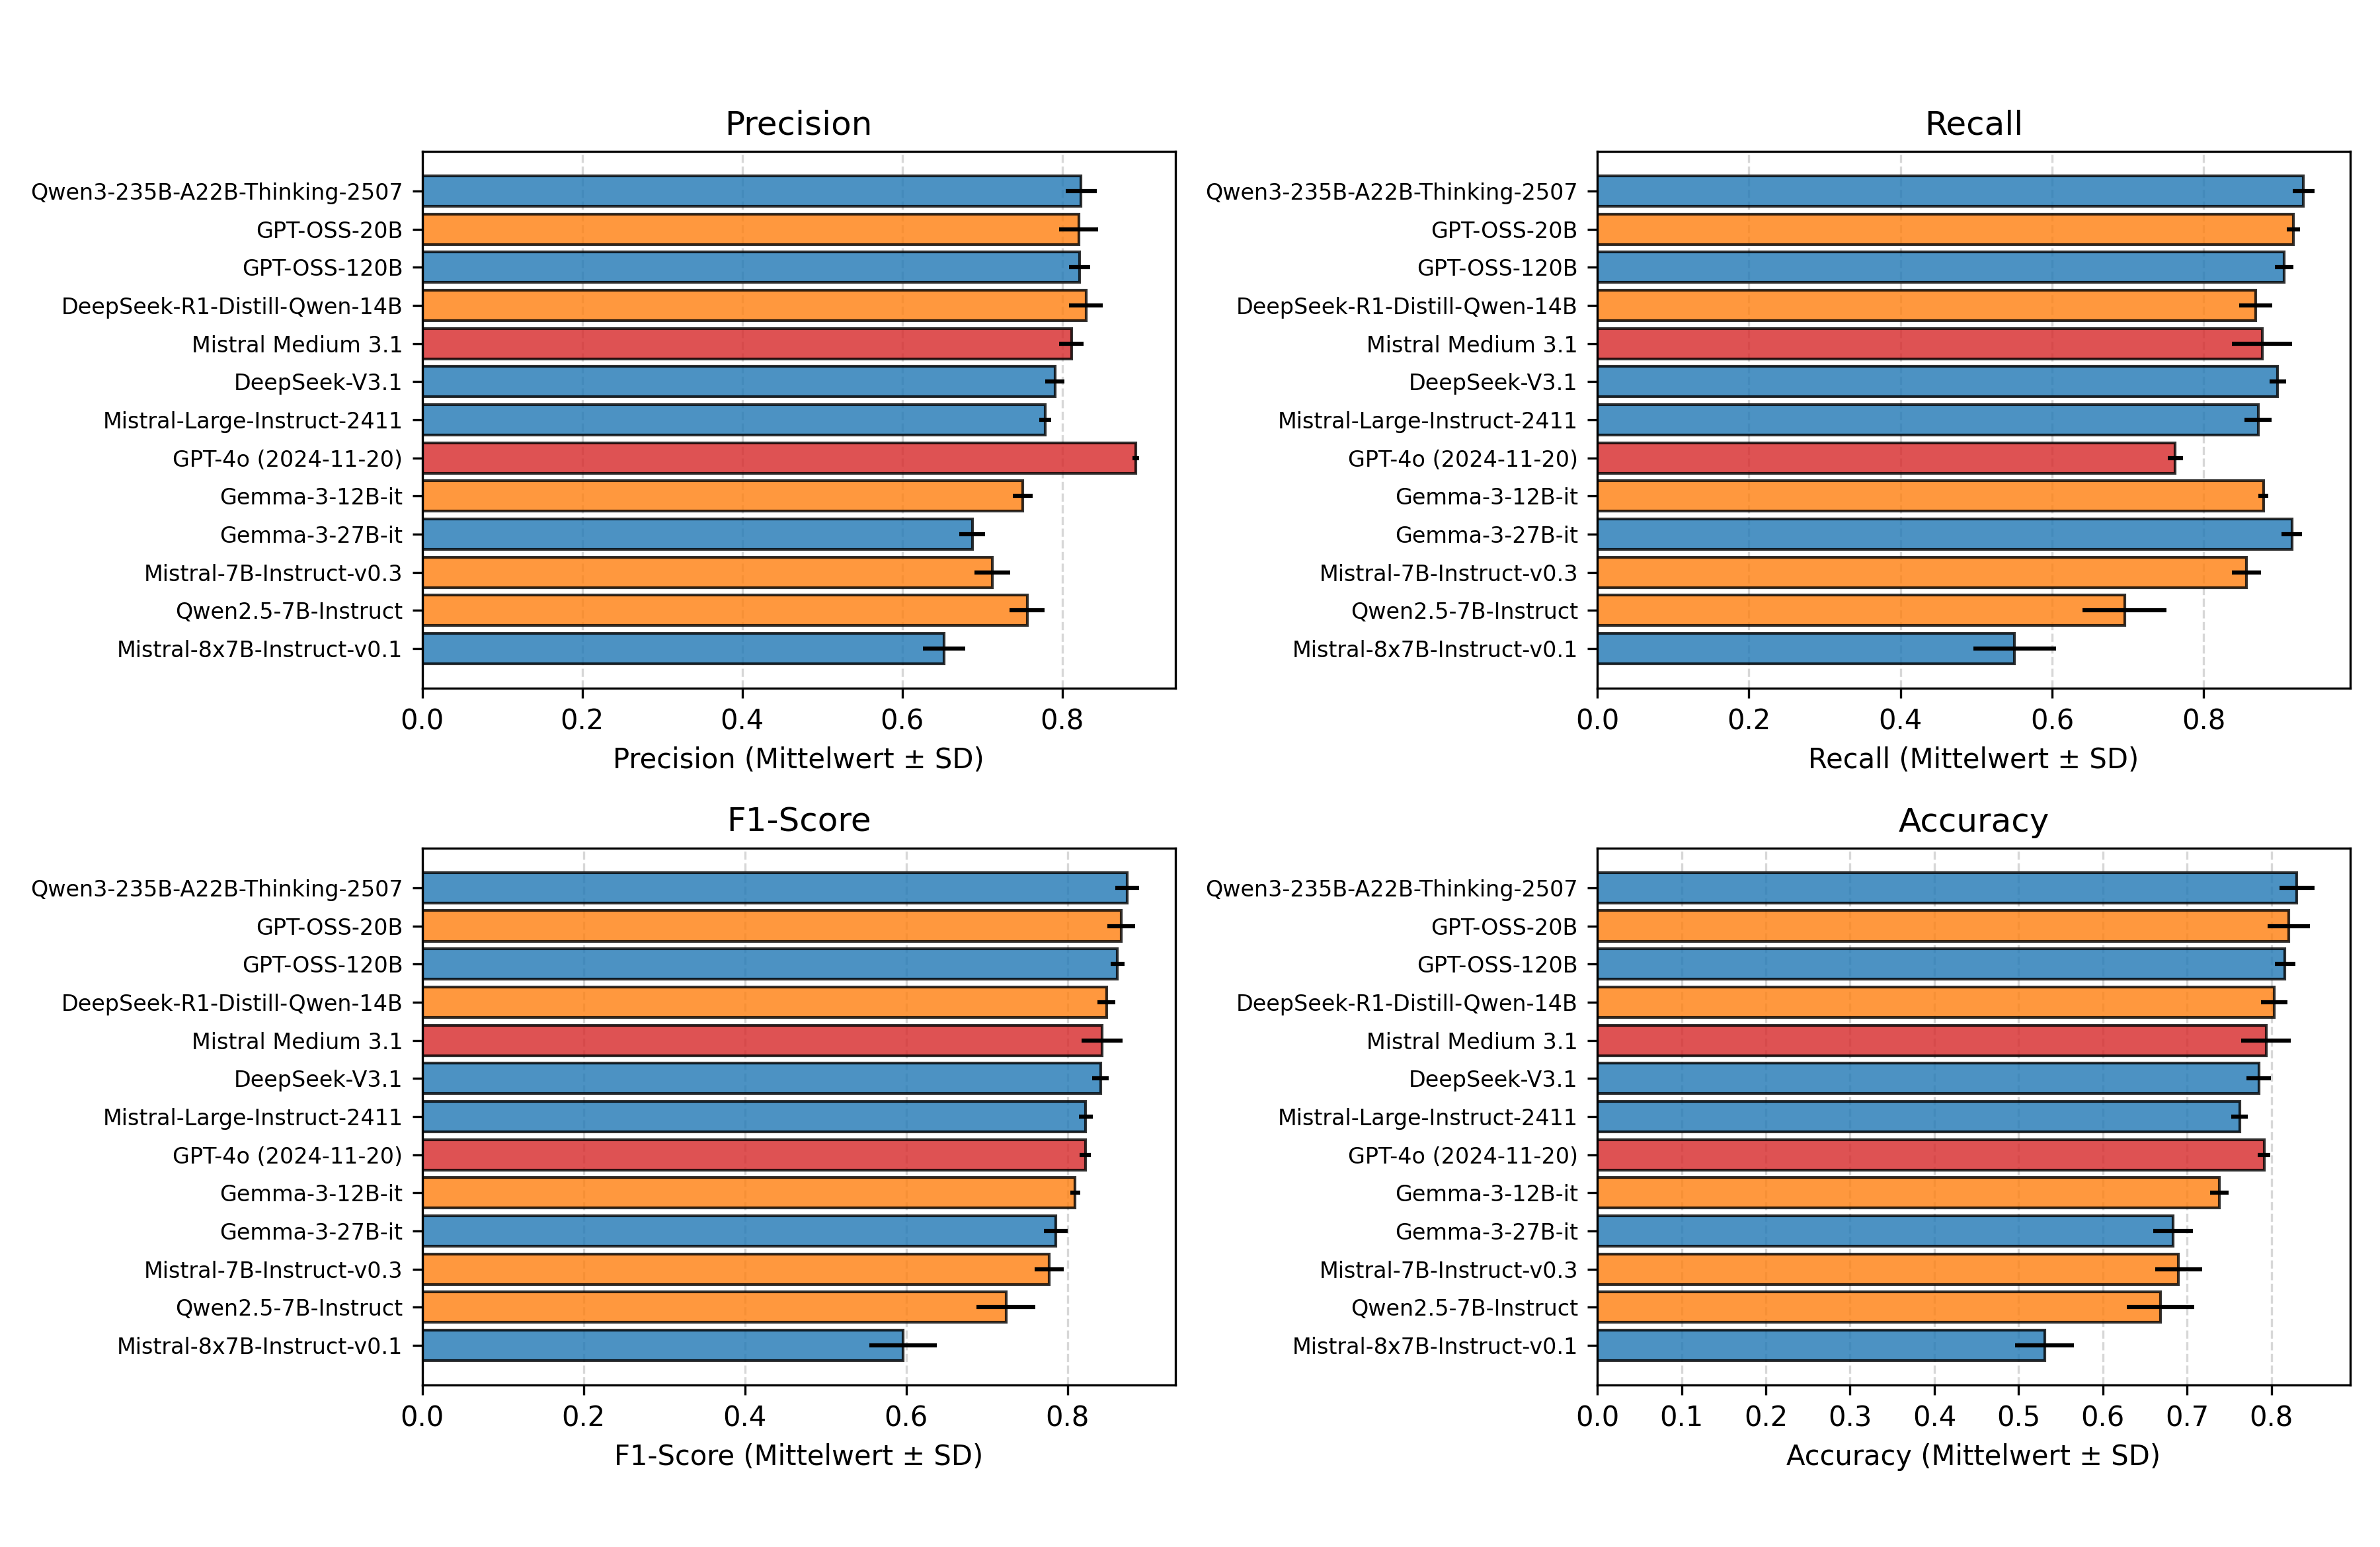
\includegraphics[width=\textwidth,trim=20 40 20 10]{images/results/evaluation_metrics_comparison}
    \caption{Durchschnittliche Metrik-Werte der untersuchten Modelle über alle Wiederholungen hinweg inklusive Standardabweichung.}
    \label{fig:results-evaluation-metrics-comparison}
\end{figure}

Insgesamt erfüllen neun der dreizehn Modelle den Zielwert von $F1-Score \geq 0{,}80$ aus Abschnitt~\ref{sec:qualitatsziele}. Besonders gut schneiden \texttt{Qwen3-235B-A22B-Thinking-2507}, \texttt{GPT-OSS-120B} und \texttt{GPT-OSS-20B} ab, die F1-Scores zwischen $0{,}862$ und $0{,}874$ erreichen. Erfreulich ist, dass auch mehrere kleinere Modelle diesen Zielwert überschreiten. Am unteren Ende des Spektrums liegt das europäische \texttt{Mixtral-8x7B-\linebreak~Instruct-v0.1}, das sowohl in Precision als auch in Recall schwach abschneidet und als einziges Modell einen F1-Score deutlich unter $0{,}60$ erzielt.

Die Abbildung zeigt zudem, dass sich die Modelle hinsichtlich Precision und Recall unterschiedlich verhalten. \texttt{GPT-4o} erreicht beispielsweise mit $0{,}892$ die höchste Precision, liegt jedoch beim Recall mit $0{,}762$ unter dem Mindestziel von $0{,}80$. Umgekehrt erzielt \texttt{Gemma-3-27B-it} einen sehr hohen Recall von $0{,}916$, wird aber durch eine niedrige Precision von $0{,}687$ ausgebremst. Modelle wie \texttt{Qwen3-235B-A22B-\linebreak~Thinking-2507}, \texttt{GPT-OSS-20B} und \texttt{DeepSeek-R1-Distill-Qwen-14B} bieten eine ausgewogene Balance und zählen deshalb zu den Spitzenreitern.

Tabelle \ref{tab:metrics-overview} fasst alle Metriken mit ihren Mittelwerten und Standardabweichungen tabellarisch zusammen. Für die weitere Analyse werden diese Werte nur noch punktuell zitiert, um Wiederholungen zu vermeiden.

\begin{table}[htbp]
    \centering
    \caption{Aggregierte Mittelwerte und Standardabweichungen der Evaluationsmetriken über alle fünf Wiederholungen hinweg.}
    \label{tab:metrics-overview}
    \begin{adjustbox}{width=\textwidth}
        \begin{tabular}{l r r r r}
            \toprule
            Modell                          & Precision         & Recall            & F1-Score          & Accuracy \\
            \midrule
            DeepSeek-V3.1                   & 0.791 $\pm$ 0.012 & 0.897 $\pm$ 0.011 & 0.841 $\pm$ 0.011 & 0.785 $\pm$ 0.015 \\
            DeepSeek-R1-Distill-Qwen-14B    & 0.829 $\pm$ 0.021 & 0.868 $\pm$ 0.022 & 0.848 $\pm$ 0.011 & 0.803 $\pm$ 0.016 \\
            Gemma-3-12B-it                  & 0.751 $\pm$ 0.013 & 0.879 $\pm$ 0.006 & 0.810 $\pm$ 0.006 & 0.738 $\pm$ 0.011 \\
            Gemma-3-27B-it                  & 0.687 $\pm$ 0.016 & 0.916 $\pm$ 0.014 & 0.785 $\pm$ 0.015 & 0.683 $\pm$ 0.023 \\
            Mistral-7B-Instruct-v0.3        & 0.712 $\pm$ 0.022 & 0.856 $\pm$ 0.019 & 0.777 $\pm$ 0.018 & 0.690 $\pm$ 0.028 \\
            Mixtral-8x7B-Instruct-v0.1      & 0.652 $\pm$ 0.027 & 0.550 $\pm$ 0.054 & 0.596 $\pm$ 0.042 & 0.531 $\pm$ 0.035 \\
            Mistral-Large-Instruct-2411     & 0.779 $\pm$ 0.008 & 0.872 $\pm$ 0.018 & 0.823 $\pm$ 0.008 & 0.762 $\pm$ 0.010 \\
            Mistral Medium 3.1              & 0.811 $\pm$ 0.015 & 0.877 $\pm$ 0.040 & 0.843 $\pm$ 0.025 & 0.794 $\pm$ 0.029 \\
            GPT-OSS-20B                     & 0.820 $\pm$ 0.024 & 0.918 $\pm$ 0.009 & 0.866 $\pm$ 0.017 & 0.821 $\pm$ 0.025 \\
            GPT-OSS-120B                    & 0.822 $\pm$ 0.013 & 0.906 $\pm$ 0.012 & 0.862 $\pm$ 0.009 & 0.816 $\pm$ 0.012 \\
            GPT-4o                          & 0.892 $\pm$ 0.004 & 0.762 $\pm$ 0.010 & 0.822 $\pm$ 0.007 & 0.791 $\pm$ 0.007 \\
            Qwen2.5-7B-Instruct             & 0.756 $\pm$ 0.022 & 0.696 $\pm$ 0.055 & 0.724 $\pm$ 0.037 & 0.668 $\pm$ 0.040 \\
            Qwen3-235B-A22B-Thinking-2507   & 0.824 $\pm$ 0.019 & 0.932 $\pm$ 0.014 & 0.874 $\pm$ 0.015 & 0.830 $\pm$ 0.021 \\
            \bottomrule
        \end{tabular}
    \end{adjustbox}
\end{table}
\section{Analyse}\label{sec:analyse}

\begin{itemize}
    \item Aufschlüsselung nach Datensätzen
    \item Aufzeigen sichtbarer Muster
\end{itemize}
\section{Robustheit}\label{sec:robustheit}

Die Robustheit der Modelle wird anhand zweier Kriterien bewertet: der Varianz der F1-Scores über die verschiedenen Seeds und der Anzahl der Retries, die erforderlich waren, um eine formatkorrekte JSON-Antwort von den \acp{LLM} in der Klassifizierungspipeline zu erhalten. Beide Größen geben Aufschluss darüber, wie stabil ein Modell im produktiven Einsatz ist.

Abbildung \ref{fig:results-evaluation-robustness-f1-std} zeigt die Standardabweichungen der F1‑Scores über fünf unabhängige Läufe mit unterschiedlichen Seeds. Die Mehrzahl der Modelle weist Werte von deutlich unter $0{,}02$ auf. Sie liefern damit weitgehend gleiche Ergebnisse, unabhängig vom gewählten Seed, und gelten als stabil. Dazu zählen \texttt{Gemma-3-12B-it}, \texttt{Mistral-Large-Instruct-2411}, \texttt{GPT-OSS-120B} und \texttt{DeepSeek-R1-Distill-\linebreak~Qwen-14B}.

\begin{figure}[h]
    \centering
    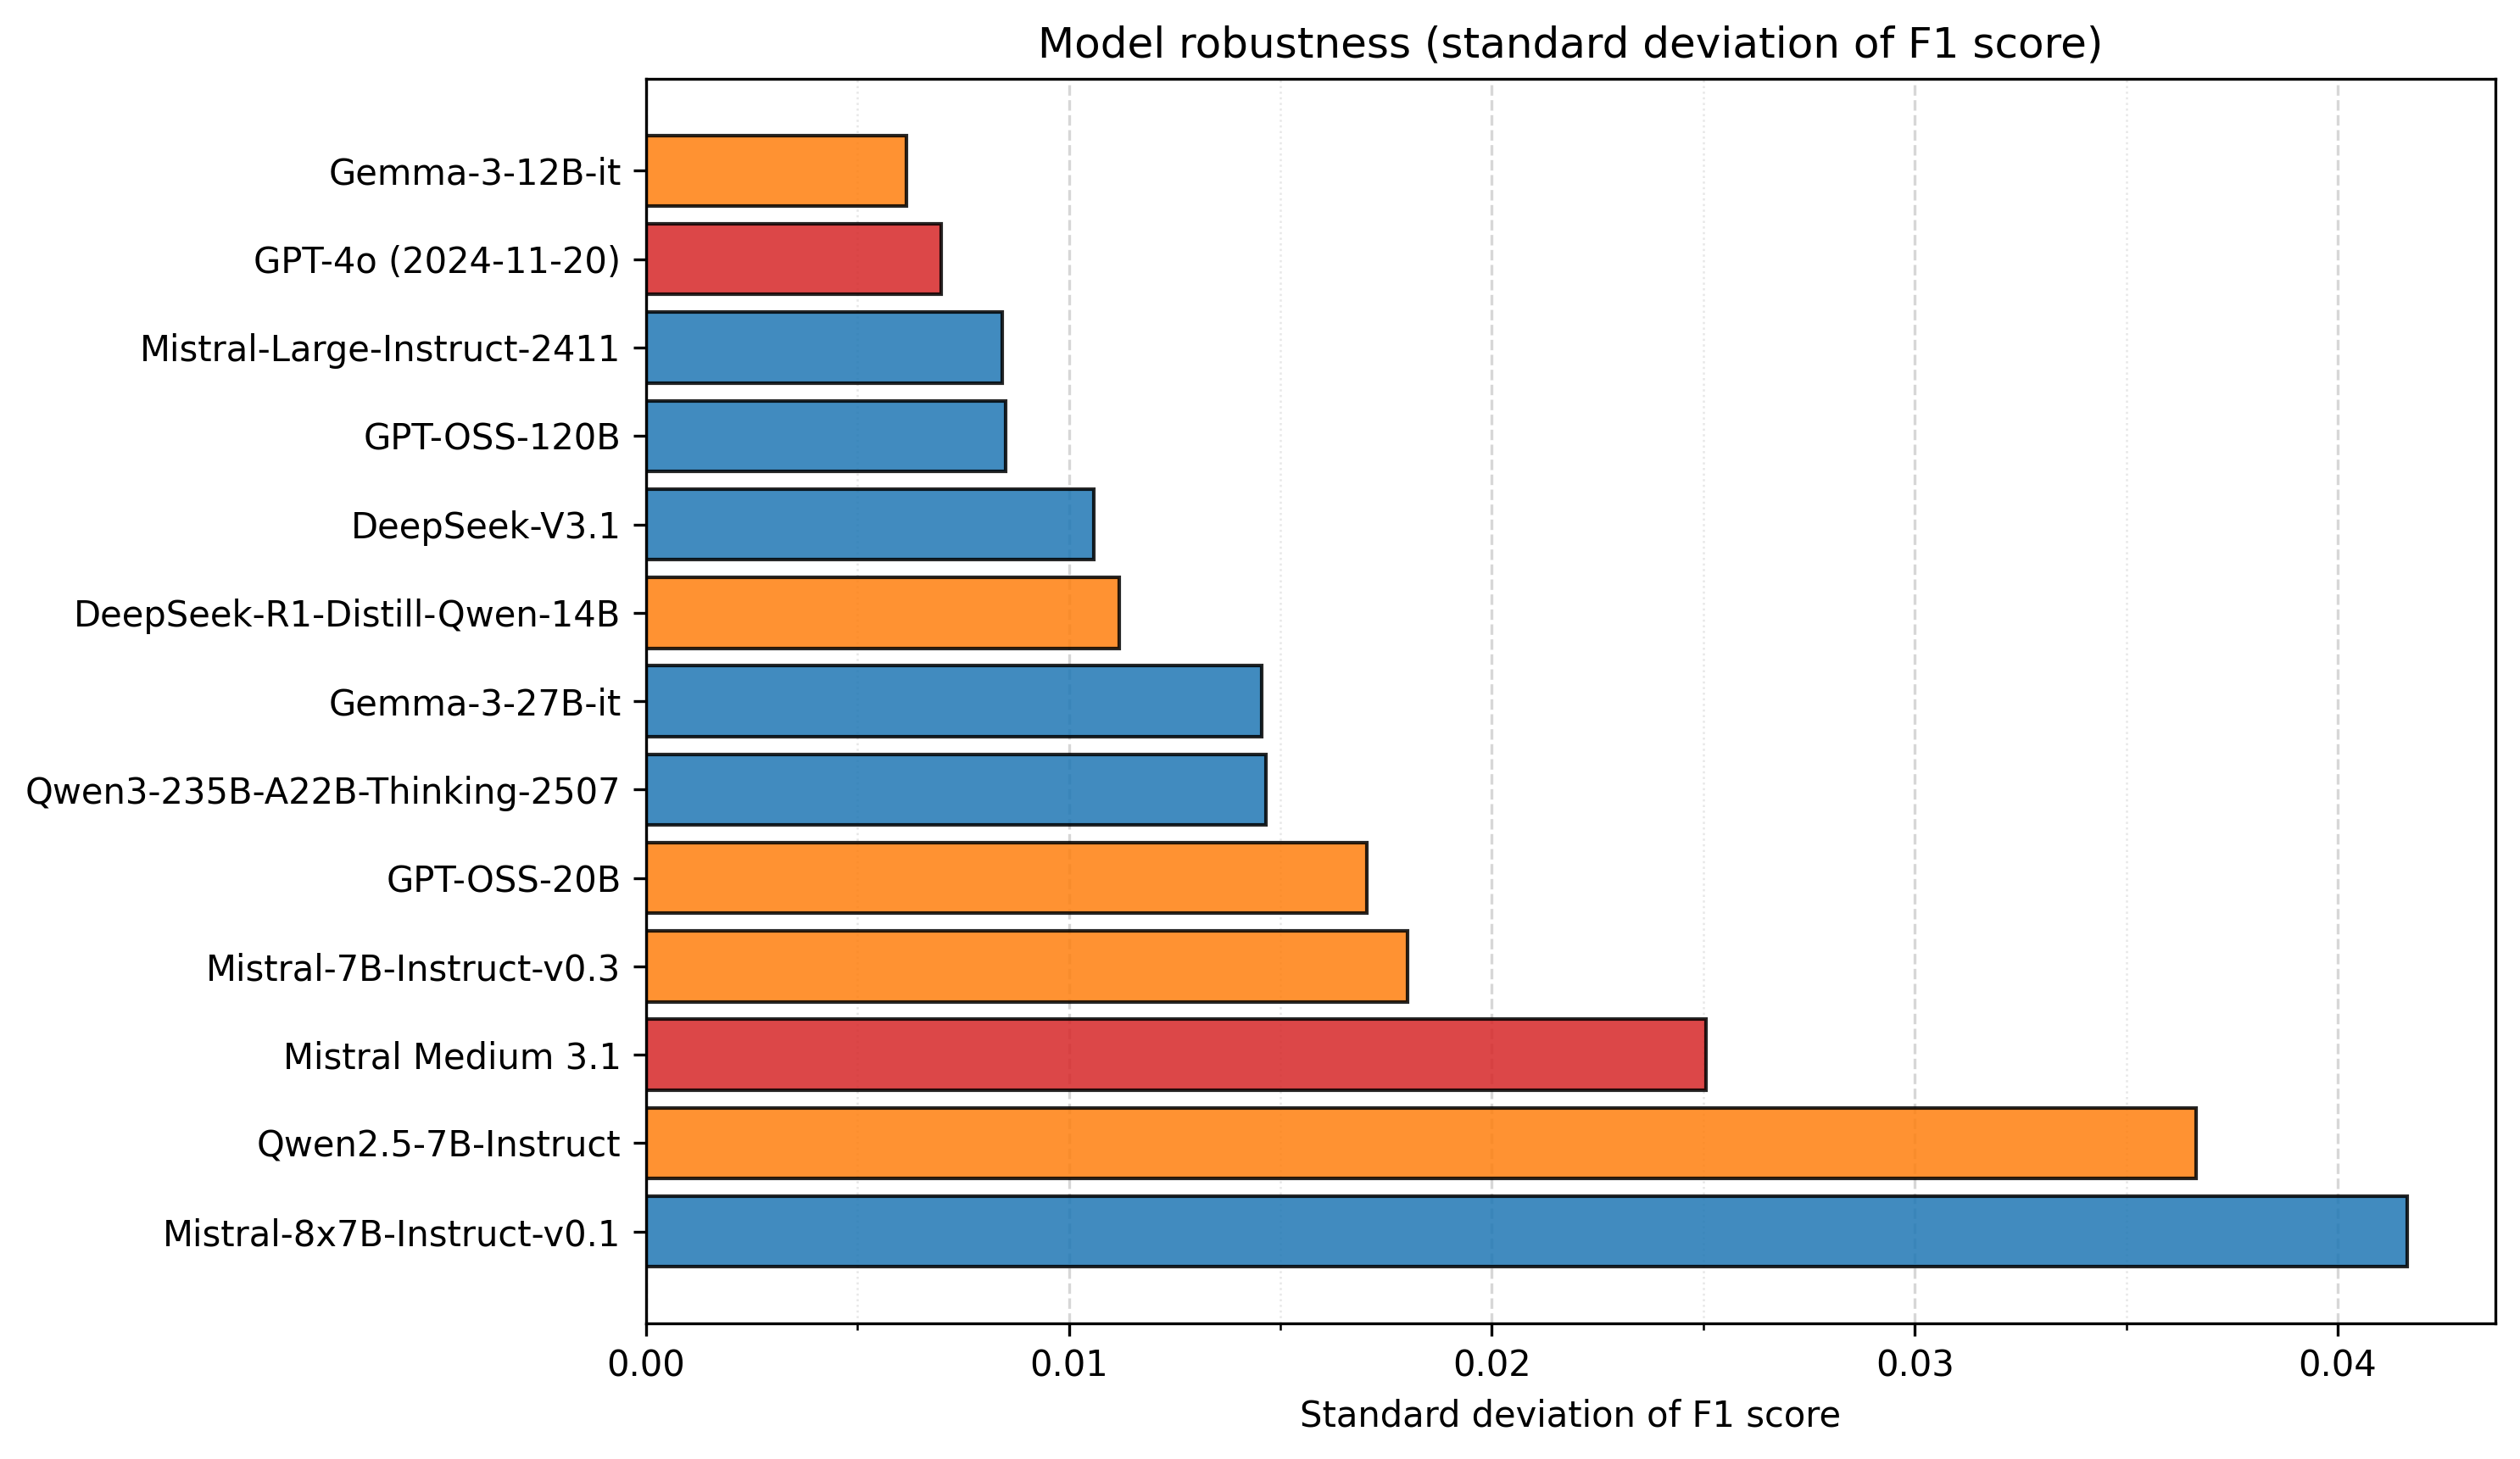
\includegraphics[width=0.7\textwidth]{images/results/evaluation_robustness_f1_std_en}
    \caption{Robustheit der Modelle gemessen an der Standardabweichung des F1-Scores über alle Wiederholungen hinweg.}
    \label{fig:results-evaluation-robustness-f1-std}
\end{figure}

Demgegenüber weisen \texttt{Mistral Medium 3.1}, \texttt{Qwen2.5-7B-Instruct} und vor allem \texttt{Mixtral-8x7B-Instruct-v0.1} mit Standardabweichungen zwischen $0{,}025$ und über $0{,}04$ eine deutlich höhere Varianz auf. Dies bedeutet, dass ihre Leistung stärker vom gewählten Seed abhängt, was die Vergleichbarkeit und Zuverlässigkeit verringert.

Neben der Varianz des F1-Scores ist auch entscheidend, wie oft das Modell nachgefragt werden muss, bis eine gültige JSON-Struktur zurückgegeben wird. Abbildung \ref{fig:results_evaluation_amount_of_retries} zeigt die durchschnittliche Anzahl notwendiger Retries pro Modell über 25 Testfälle. Die meisten Modelle lieferten bereits im ersten Versuch oder nach maximal einem zusätzlichen Aufruf eine korrekte Antwort. Hervorzuheben sind\linebreak~\texttt{DeepSeek-R1-Distill-Qwen-14B}, \texttt{GPT-4o}, \texttt{Gemma-3-12B-it} und \texttt{Mistral-\linebreak~Large-Instruct-2411}, die keinerlei Retries benötigten.

\begin{figure}[h]
    \centering
    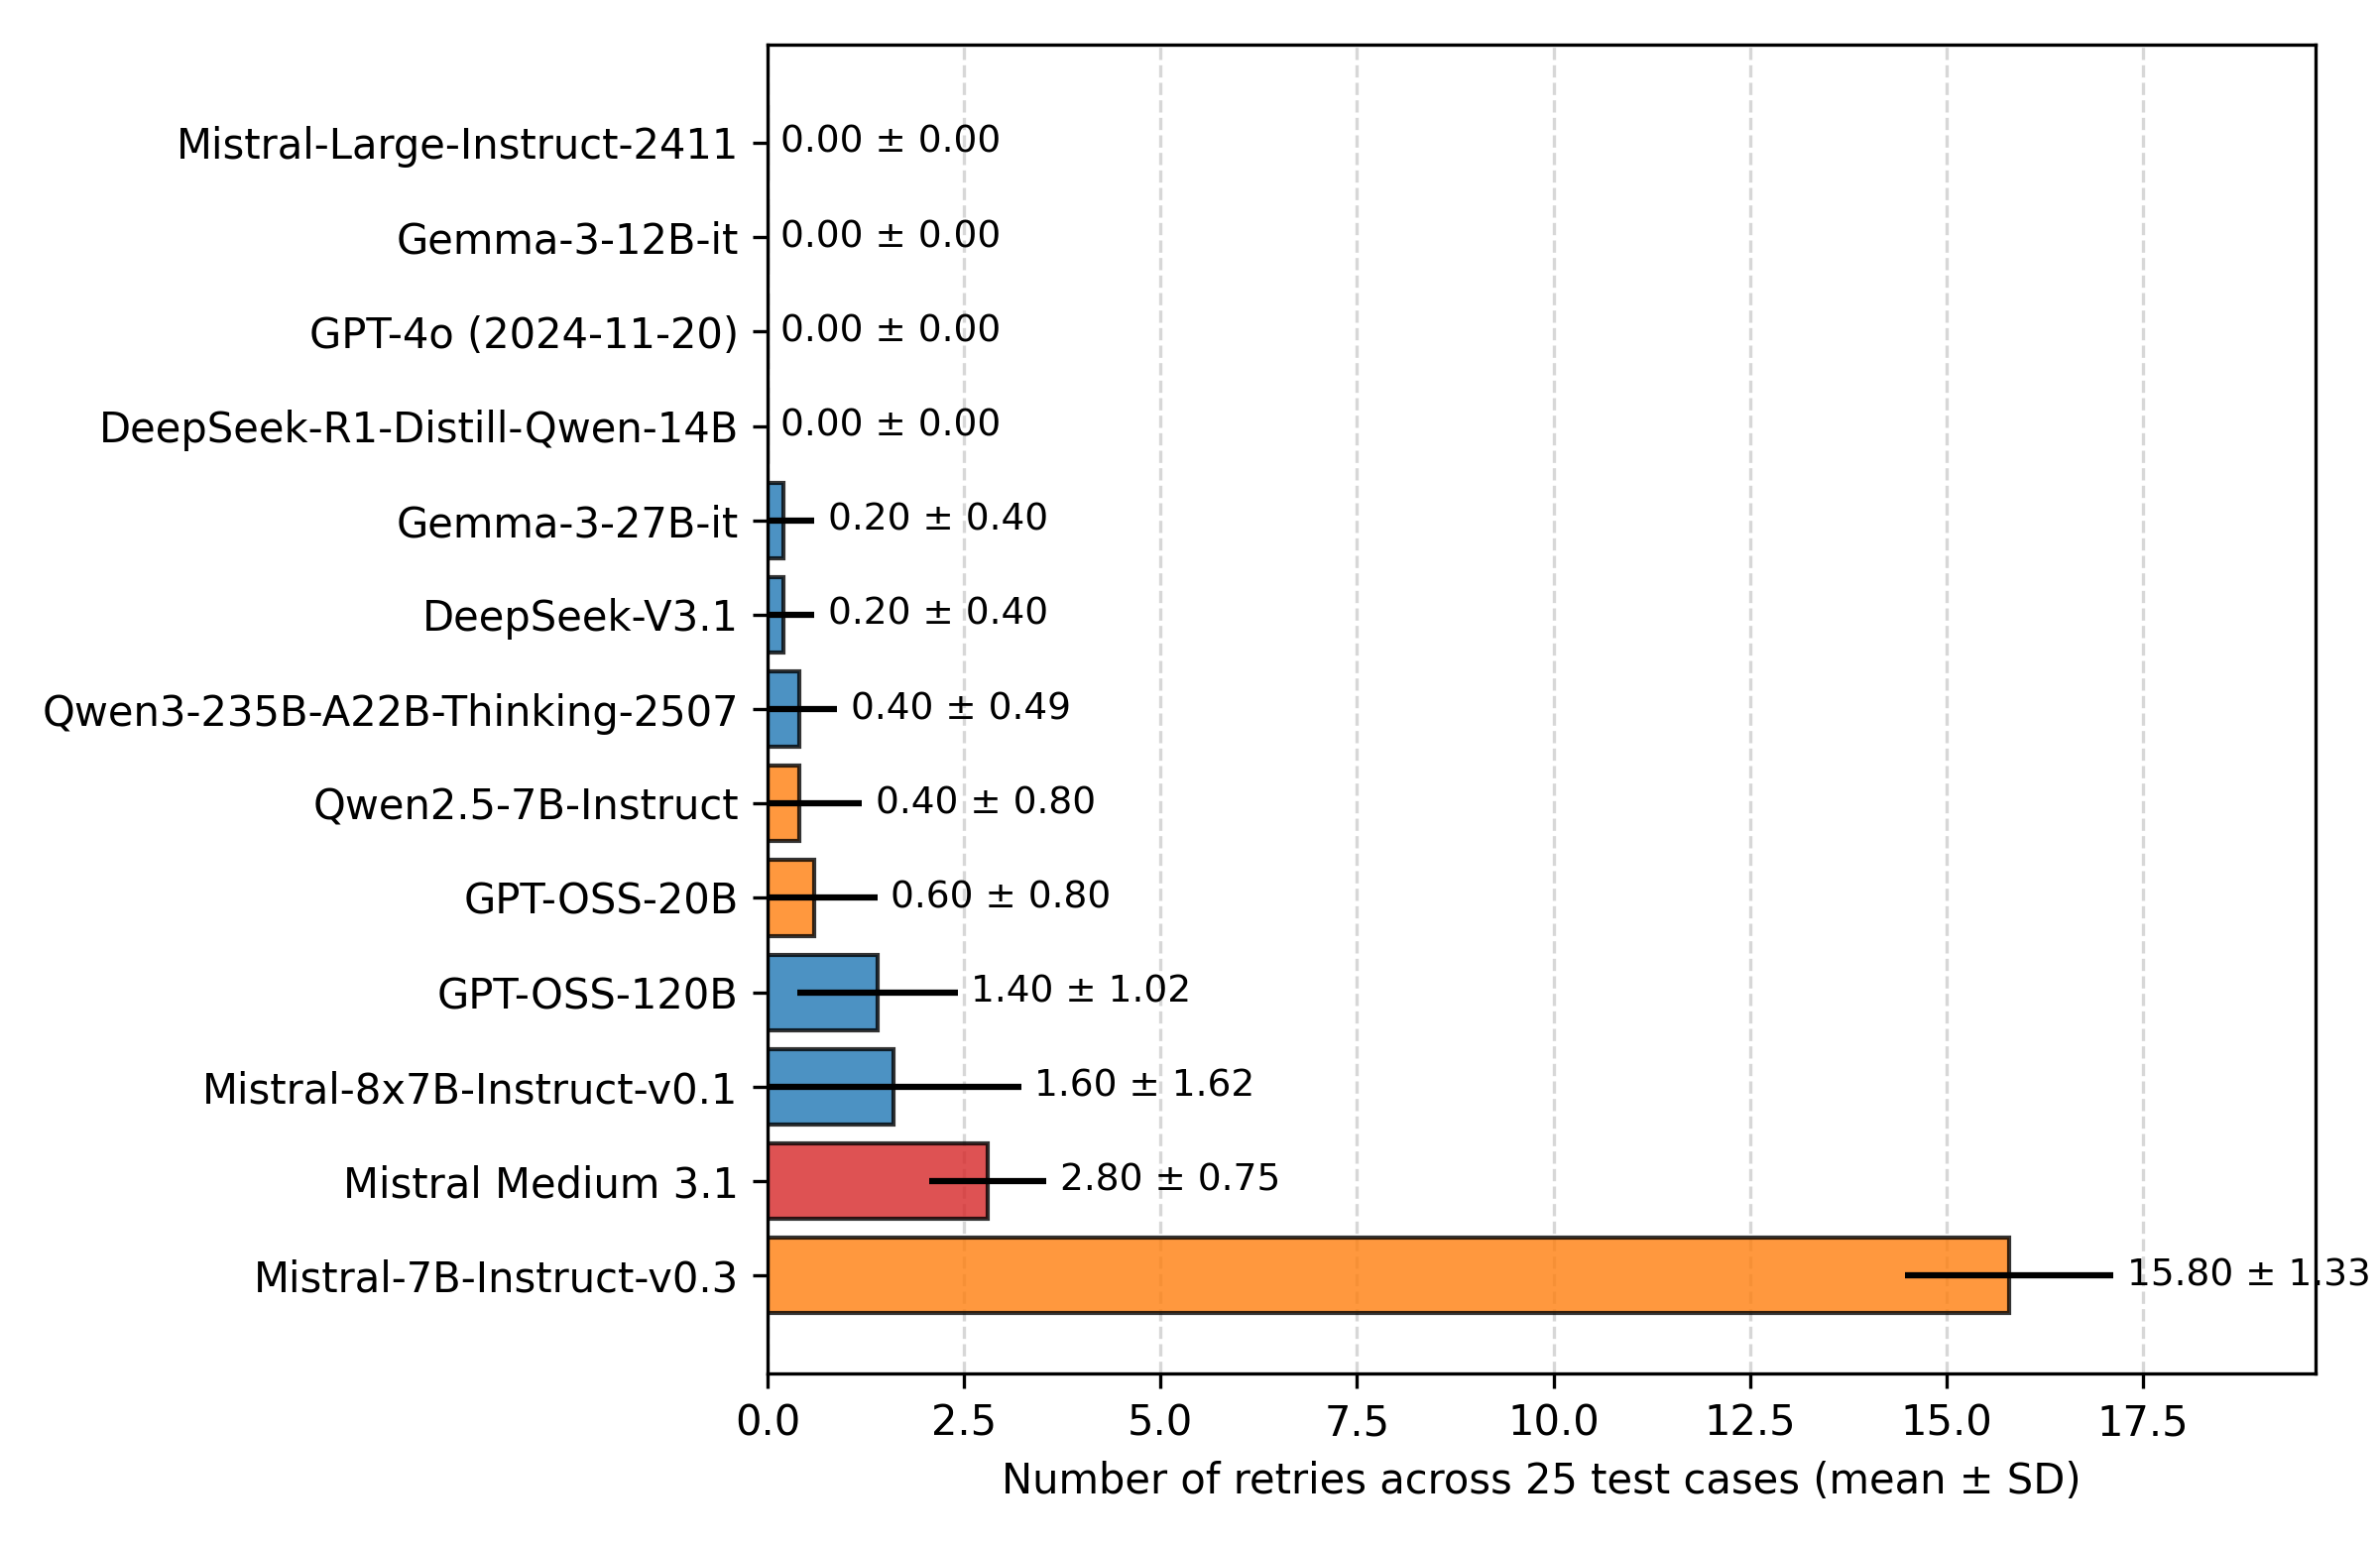
\includegraphics[width=0.7\textwidth]{images/results/evaluation_amount_of_retries_en}
    \caption{Durchschnittliche Anzahl der Retries, die notwendig waren, um für alle 25 Testfälle eine formatkorrekte JSON-Antwort zu erhalten.}
    \label{fig:results_evaluation_amount_of_retries}
\end{figure}

Am anderen Ende des Spektrums steht \texttt{Mistral-7B-Instruct-v0.3}, das im Mittel $15{,}8$ zusätzliche Aufrufe benötigte, was im Durchschnitt etwa $0{,}63$ Retries pro Testfall entspricht. Diese hohe Zahl verdeutlicht, dass das Modell Schwierigkeiten hat, die vorgegebenen Formatierungsregeln zuverlässig einzuhalten.

In Kombination mit der geringen Varianz sind \texttt{Gemma-3-12B-it}, \texttt{Mistral-Large-\linebreak~Instruct-2411} und \texttt{DeepSeek-R1-Distill-Qwen-14B} die robustesten Modelle: Sie liefern konsistente Ergebnisse und halten das Ausgabeschema zuverlässig ein. Modelle wie \texttt{Mistral Medium 3.1}, \texttt{Qwen2.5-7B-Instruct} und \texttt{Mixtral-8x7B-\linebreak~Instruct-v0.1} sind hingegen anfälliger für Schwankungen und erfordern häufiger Wiederholungen.
\section{Fallstudien}\label{sec:fallstudien}

\begin{itemize}
    \item Hier werde ich (wahrscheinlich 2--3) spezifische exemplarische Ergebnisse von Testcases heraussuchen und genauer unter die Lupe nehmen. Was ist hier besonders aufgefallen oder interessant?
    \item Hier kann ich die Bilder mit den Highlights hernehmen
    \item Idealerweise habe ich Beispiele für 1. TN, 2. FP aber plausible Erklärung und 3. FN
\end{itemize}
\section{Antworten auf Forschungsfragen}\label{sec:antworten-auf-forschungsfragen}

Basierend auf den vorstehenden Auswertungen können die in \ref{sec:zielsetzung-und-beitrage} formulierten Forschungsfragen beantwortet werden. Die nachfolgenden Antworten berücksichtigen sowohl die quantitativen Ergebnisse als auch qualitative Beobachtungen aus den Fallstudien und ordnen sie unter berücksichtigung der Qualitätsziele aus Abschnitt \ref{sec:qualitatsziele} ein.

\paragraph{UF1: Wie gut schneiden europäische Modelle im Vergleich zu internationalen Modellen ab?}

Die europäischen Modelle zeigen eine große Spannweite in ihrer Leistungsfähigkeit. Wie in Abschnitt~\ref{sec:qualitatsziele} dargelegt, gelten als Qualitätsziele ein Recall von mindestens $0{,}80$ mit angestrebtem Bereich ab $0{,}85$, eine Precision von mindestens $0{,}75$, ein F1-Score von mindestens $0{,}80$ sowie höchstens $1{,}5$ \acp{FP} je Prozess.

Das proprietäre \texttt{Mistral Medium 3.1} ist mit einem F1-Score von $0{,}843$ und einem Recall von $0{,}877$ das leistungsstärkste \ac{EU}-Modell. Es übertrifft \texttt{GPT-4o} beim F1-Score und beim Recall, liegt jedoch hinter den besten internationalen Modellen. Im Rahmen der Qualitätsziele erfüllt \texttt{Mistral Medium 3.1} alle Kriterien, denn der Recall liegt im angestrebten Bereich, die Precision von $0{,}811$ überschreitet die Untergrenze und der F1-Score liegt über dem Zielwert.

\texttt{Mistral-Large-Instruct-2411} bewegt sich mit Blick auf F1-Score und Recall im Mittelfeld der getesteten Modelle und liegt knapp vor \texttt{GPT-4o}. Die Qualitätsziele werden erreicht, denn der Recall beträgt $0{,}872$ und erreicht das Mindestniveau, die Precision liegt mit $0{,}779$ über der Untergrenze und der F1-Score von $0{,}823$ erfüllt das Ziel.

Das kleine Modell \texttt{Mistral-7B-Instruct-v0.3} erzielt mit F1-Score $0{,}777$ und Recall $0{,}856$ – insbesondere für die Größe – solide Werte und ordnet sich insgesamt im unteren Mittelfeld ein. Das Recall-Ziel wird erreicht, die Precision von $0{,}712$ unterschreitet jedoch die Untergrenze, und der F1-Score bleibt dadurch unter dem Zielwert.

Das \ac{MoE}-Modell \texttt{Mixtral-8x7B-Instruct-v0.1} schneidet mit F1-Score $0{,}596$ und Recall $0{,}550$ deutlich schlechter ab und bildet das Schlusslicht der getesteten Modelle. Sämtliche Zielwerte werden verfehlt, da auch die Precision mit $0{,}652$ unter der Untergrenze liegt.

In jeder Größenklasse finden sich internationale Modelle, die die europäischen Modelle übertreffen. \texttt{Qwen3-235B-A22B-Thinking-2507} erreicht einen Recall von $0{,}932$ und einen F1-Score von $0{,}874$ und liegt damit klar im Zielbereich. \texttt{GPT-OSS-20B} und \texttt{GPT-OSS-120B} erfüllen mit Recall $0{,}918$ beziehungsweise $0{,}906$ und F1-Score $0{,}866$ beziehungsweise $0{,}862$ sämtliche Kriterien. \texttt{GPT-4o} erfüllt mit Precision $0{,}892$ und F1-Score $0{,}822$ die entsprechenden Zielwerte, unterschreitet jedoch das Recall-Mindestniveau mit $0{,}762$.

Damit lässt sich festhalten, dass die internationalen Modelle im Mittel eine höhere Klassifikationsqualität bieten. \ac{EU}-Modelle können vor allem durch ihre datenschutzfreundliche Bereitstellung und ihren Standortvorteil punkten. Leistungsmäßig erfüllen \texttt{Mistral Medium 3.1} und \texttt{Mistral-Large-Instruct-2411} die Qualitätsziele, während \texttt{Mistral-7B-Instruct-v0.3} und \texttt{Mixtral-8x7B-Instruct-\linebreak~v0.1} diese nicht vollständig erreichen.

\paragraph{UF2: Wie unterschieden sich große und kleine Modelle in ihrer Leistungsfähigkeit?}

Die Gegenüberstellung kleiner Modelle mit $\leq 25B$ Parametern und großer Modelle mit $> 25B$ Parametern ergab kaum Unterschiede im Durchschnitt. Der mittlere F1-Score liegt mit $0{,}805$ bei den kleinen und $0{,}806$ bei den großen Modellen praktisch gleichauf. Ohne das deutlich unterdurchschnittliche \texttt{Mixtral-\linebreak~8x7B-Instruct-v0.1} steigt der Durchschnitt der großen Modelle auf $0{,}836$, was zeigt, dass größere Modelle tendenziell bessere Leistungen erbringen können. Die Recall-Werte der kleinen Modelle von durchschnittlich $0{,}843$ übertreffen die der großen Modelle von $0{,}839$ leicht, während Precision und Accuracy in beiden Gruppen vergleichbar sind. Auffällig ist die höhere Varianz der großen Modelle: die Standardabweichung des F1-Scores beträgt $0{,}089$, bei den kleinen lediglich $0{,}057$. Dies ist vor allem auf das Ausreißermodell \texttt{Mixtral-8x7B-Instruct-v0.1} zurückzuführen. Bei den Bestwerten liegen die Gruppen einigermaßen dicht beieinander: das beste kleine Modell \texttt{GPT-OSS-20B} erzielt einen F1-Score von $0{,}866$ und einen Recall von $0{,}918$, während das beste große Modell \texttt{Qwen3-235B-A22B-Thinking-\linebreak~2507} einen F1-Score von $0{,}874$ und einen Recall von $0{,}932$ erreicht.

Die Analyse zeigt, dass die Modellgröße allein kein entscheidender Faktor für die Klassifikationsleistung ist. Vielmehr sind Trainingsdaten, Feinabstimmung und Architektur entscheidender. Leistungsfähige kleine Modelle können mit den großen mithalten und sind im praktischen Einsatz ressourcenschonender.

\paragraph{UF3: Welche Open-Source-Modelle (insbesondere aus der EU) erzielen die besten Ergebnisse?}

Unter den offenen Modellen erzielen \texttt{Qwen3-235B-A22B-\linebreak~Thinking-2507}, \texttt{GPT-OSS-20B} und \texttt{DeepSeek-R1-Distill-Qwen-14B} die besten Ergebnisse. \texttt{Qwen3-235B-A22B-Thinking-2507} erreicht mit einem F1-Score von $0{,}874$, einem Recall von $0{,}932$ und einer Precision von $0{,}824$ den Spitzenplatz. \texttt{GPT-OSS-20B} folgt mit F1 $0{,}866$, Recall $0{,}918$ und Precision $0{,}820$. Auch das kleinere \texttt{DeepSeek-R1-Distill-Qwen-14B} überzeugt mit einem F1-Score von $0{,}848$ und einer Precision von $0{,}829$. Diese Modelle übertreffen die proprietären Benchmarks und erfüllen die Qualitätsziele klar.

Die europäischen Open-Source-Modelle weisen hingegen ein heterogenes Leistungsbild auf. \texttt{Mistral-Large-Instruct-2411} ist mit einem F1-Score von $0{,}823$ und einer Precision von $0{,}779$ das leistungsstärkste offene EU-Modell und erfüllt alle Qualitätsziele. \texttt{Mistral-7B-Instruct-v0.3} erreicht zwar einen Recall von $0{,}856$, bleibt mit einer Precision von $0{,}712$ und F1-Score von $0{,}777$ aber unter den Zielwerten. \texttt{Mixtral-8x7B-Instruct-v0.1} schneidet mit einem F1-Score von $0{,}596$ und Recall von $0{,}550$ deutlich schlechter ab und verfehlt alle Ziele.

Insgesamt dominieren bei den Open-Source-Modellen die chinesischen Qwen-\linebreak~Varianten und die GPT-OSS-Modelle das Feld, während europäische Modelle im Schnitt hinter den internationalen Spitzenreitern zurückbleiben.

\paragraph{UF4: Wie gut schneiden Open-Source-Modelle gegenüber kommerziellen Modellen wie GPT-4o ab?}

Der Vergleich zeigt, dass mehrere Open-Source-Modelle die kommerziellen Vertreter in der Klassifikationsqualität übertreffen. Zu den proprietären Modellen im Vergleichsfeld zählen \texttt{GPT-4o} und das europäische \texttt{Mistral Medium 3.1}. \texttt{Mistral Medium 3.1} erreicht einen F1-Score von $0{,}843$, einen Recall von $0{,}877$ und eine Precision von $0{,}811$ und liegt damit vor \texttt{GPT-4o}, das einen F1-Score von $0{,}822$, einen Recall von $0{,}762$ und eine sehr hohe Precision von $0{,}892$ erzielt.

Unter den offenen Modellen führen \texttt{Qwen3-235B-A22B-Thinking-2507} mit einem F1-Score von $0{,}874$, einem Recall von $0{,}932$ und einer Precision von $0{,}824$ sowie \texttt{GPT-OSS-20B} mit einem F1-Score von $0{,}866$, einem Recall von $0{,}918$ und einer Precision von $0{,}820$. Das kleinere \texttt{DeepSeek-R1-Distill-Qwen-14B} liegt beim F1-Score mit $0{,}848$ ebenfalls über \texttt{GPT-4o}, erreicht jedoch nicht dessen außergewöhnlich hohe Precision. Gleichzeitig ist die Spannweite innerhalb der Open-Source-Kategorie größer, wie das schwache Abschneiden von \texttt{Mixtral-8x7B-\linebreak~Instruct-v0.1}.

Insgesamt zeigen hochwertige Open-Source-Modelle die stärkste Balance aus hohem Recall und hohem F1-Score und erfüllen die Qualitätsziele klar, während\linebreak~\texttt{GPT-4o} durch exzellente Precision überzeugt, aber aufgrund des niedrigen Recalls häufiger kritische Aktivitäten übersieht. \texttt{Mistral Medium 3.1} belegt, dass ein kommerzielles \ac{EU}-Modell die Ziele ebenfalls erfüllt und im F1-Score und Recall vor \texttt{GPT-4o} liegt.

Auf Basis der durchgeführten Experimente, Analysen und Antworten auf die Unterfragen lässt sich die Hauptforschungsfrage beantworten im Folgenden beantworten.

\paragraph{FF1: Wie zuverlässig identifizieren LLM DSGVO-kritische Aktivitäten in BPMN-Prozessmodellen?}

Die Ergebnisse zeigen, dass moderne \acp{LLM} \ac{DSGVO}-\linebreak~kritische Aktivitäten mit hoher Zuverlässigkeit erkennen können. Insgesamt erfüllten neun von dreizehn Modellen den F1-Score-Zielwert von mindestens $0{,}80$, darunter auch mehrere kleinere Modelle. Die besten Modelle – \texttt{Qwen3-235B-A22B-\linebreak~Thinking-2507}, \texttt{GPT-OSS-20B}, \texttt{DeepSeek-R1-Distill-Qwen-14B} und \texttt{Mistral Medium 3.1} – erzielten F1-Scores zwischen $0{,}843$ und $0{,}874$ sowie Recall-Werte von $0{,}868$ bis $0{,}932$, überschritten damit deutlich die aus der Literatur abgeleiteten Referenzwerte und erfüllten die Qualitätsziele. Gleichzeitig gibt es Modelle wie \texttt{Mixtral-8x7B-Instruct-v0.1} und \texttt{Qwen2.5-7B-Instruct}, die mit F1-Scores unter $0{,}60$ beziehungsweise $0{,}73$ und Recall unter $0{,}70$ deutlich abfallen.

Die Robustheitsanalyse zeigt, dass die meisten Modelle eine sehr geringe Varianz zwischen verschiedenen Seeds aufweisen: die Standardabweichung des F1-Scores liegt oft unter $0{,}02$. Modelle wie \texttt{Gemma-3-12B-it}, \texttt{Mistral-Large-\linebreak~Instruct-2411} und \texttt{DeepSeek-R1-Distill-Qwen-14B} benötigten zudem keine Retries, um eine korrekte JSON-Antwort zu liefern, was ihre Zuverlässigkeit unterstreicht. Dagegen reagieren \texttt{Mistral Medium 3.1}, \texttt{Qwen2.5-7B-Instruct} und vor allem \texttt{Mixtral-8x7B-Instruct-v0.1} empfindlicher auf den Seed und erfordern bei Formatierung der Ausgabe teilweise zahlreiche Wiederholungen.

Die Fallstudien verdeutlichen typische Fehlerbilder. Im Testfall \enquote{Sales Warehouse} erkannte \texttt{Qwen3-235B-A22B-Thinking-2507} alle kritischen Aktivitäten, markierte aber zusätzlich das Versenden eines Produkts als kritisch, weil das Modell die Nutzung der Kundenadresse als potenzielle Datenverarbeitung interpretierte, während bei der Modellierung lediglich an einen logistischen Schritt gedacht war. Dieses \ac{FP} ist angesichts des angestrebten hohen Recalls akzeptabel. Im Szenario \enquote{Marketing-Kampagne} identifizierte \texttt{GPT-OSS-20B} die anonymisierte Auswertung von Klickraten fälschlich als kritisch, da die notwendigen Kontextinformationen im \ac{BPMN}-Modell fehlten. Umgekehrt zeigte der Testfall \enquote{Karten-App – Standort erfassen}, dass \texttt{Mistral-Large-Instruct-2411} trotz vorhandener Datenassoziationen die zweite Aktivität \enquote{Route berechnen} nicht als kritisch markierte. Dieses \ac{FN} widerspricht dem Hauptziel eines maximalen Recalls und weist auf Schwächen bei der Erkennung von Datenflüssen über mehrere Schritte hin.

Zusammenfassend lässt sich festhalten, dass \acp{LLM} \ac{DSGVO}-kritische Aktivitäten in \ac{BPMN}-Prozessmodellen zuverlässig identifizieren können, sofern hochwertige Modelle eingesetzt werden. Die Top-Modelle erfüllen die definierten Qualitätsziele mit Recall-Werten über $0{,}90$ und akzeptabler Precision, die Zahl der \ac{FP} pro Prozess bleibt moderat. Dennoch sind eine sorgfältige Modellwahl und eine nachgelagerte menschliche Prüfung ratsam, um die verbleibenden \acp{FP} und \ac{FN} zu adressieren und die Ergebnisse in den jeweiligen Anwendungskontext einzuordnen.

\chapter{Diskussion}\label{ch:diskussion}

\section{Interpretation der Befunde}\label{sec:interpretation-der-befunde}

\begin{itemize}
    \item Einordnung der Rangfolge der LLMs
    \item Besonderheiten der Modellfamilien (Bspw. wie groß ist der Unterschied von Groß gegen Klein?)
    \item Es gab Prozesse in denen ich eine Aktivität nicht als kritisch gelabelt habe, aber das LLM in der Evaluierung das als kritisch mit einer validen Begründung klassifiziert hat, man könnte die Testdaten also noch anpassen, wenn die Begründung des LLMs überzeugt (Ich weiß nicht wie sinnvoll das ist hier zu thematisieren) -> hier eher in die Richtung gehen, dass lieber mehrere Personen labeln als auf die Anpassung der Datensätze zu gehen.
\end{itemize}
\section{Hoher Recall vs. Präzision}\label{sec:hoher-recall-vs.-prazision}

\begin{itemize}
    \item Beobachtung ausformulieren, dass einige Testfälle als fehlerhaft eingeordnet wurden, weil es False-Positives gab, obwohl es keine False-Negatives gab. Es wurden also alle Aktivitäten gefunden, die gefunden werden sollten, nur halt noch mehr on top.
    \item Einordnung der FP-Last pro Prozess (Lieber False Positives, als dass etwas übersehen wird, Ziel war sowieso ein Vorscreening), Diskussion darüber wie nützlich hohe Recall Werte sind
\end{itemize}
\section{EU-Modelle}\label{sec:eu-modelle}

\begin{itemize}
    \item Analyse der EU-Open-Source-Modelle in Bezug auf Precision, Recall und Stabilität in Bezug auf die anderen Modelle
    \item Wie gut haben sich die EU Modelle im Vergleich zu den anderen geschlagen
\end{itemize}
\section{Open-Source Modelle}\label{sec:open-source-modelle}

\begin{itemize}
    \item Analyse der Open-Source-Modelle in Bezug auf Precision, Recall und Stabilität in Bezug auf kommerzielle Modelle
    \item Wie gut haben sich die Open-Source-Modelle im Vergleich zu den anderen geschlagen
\end{itemize}
\section{Modellgrößen}\label{sec:modellgroen}

\begin{itemize}
    \item Selbst hosten von Modellen diskutieren. Ist es realistisch die Modelle selbst zu hosten, welche gut performt haben? Reichen die kleinen Varianten der Modelle oder muss man schon die großen Modelle benutzen, um gute Ergebnisse zu erzielen
\end{itemize}
\section{Grenzen}\label{sec:grenzen}

\begin{itemize}
    \item Wären Grenzen wie BPMN-Modellgröße im Zusammenhang mit der Kontextlänge des LLM interessant?
    \item Keine aussagekräftige Rechtsberatung, sondern stand jetzt eher ein Vorscreening, was nochmal überprüft werden muss
    \item ggf. notwendige Anonymisierung von Prozessen diskutieren (Wenn das in BPMN Modellen überhaupt ein Problem ist)
\end{itemize}
\section{Zusammenfassung der Ergebnisse}\label{sec:ueberblick}

Für jedes der 13 untersuchten Modelle wurden fünf unabhängige Läufe mit unterschiedlichen Seeds durchgeführt. Abbildung \ref{fig:results-evaluation-metrics-comparison} visualisiert die mittleren Werte für Precision, Recall, F1-Score und Accuracy jeweils inklusive Standardabweichung über alle Wiederholungen hinweg. Für einen besseren Vergleich sind proprietäre Modelle rot, kleinere Modelle orange und größere Modelle blau eingefärbt. Die Einteilung entspricht der in Kapitel~\ref{ch:modellauswahl} beschriebenen Kategorisierung.

\begin{figure}[h]
    \centering
    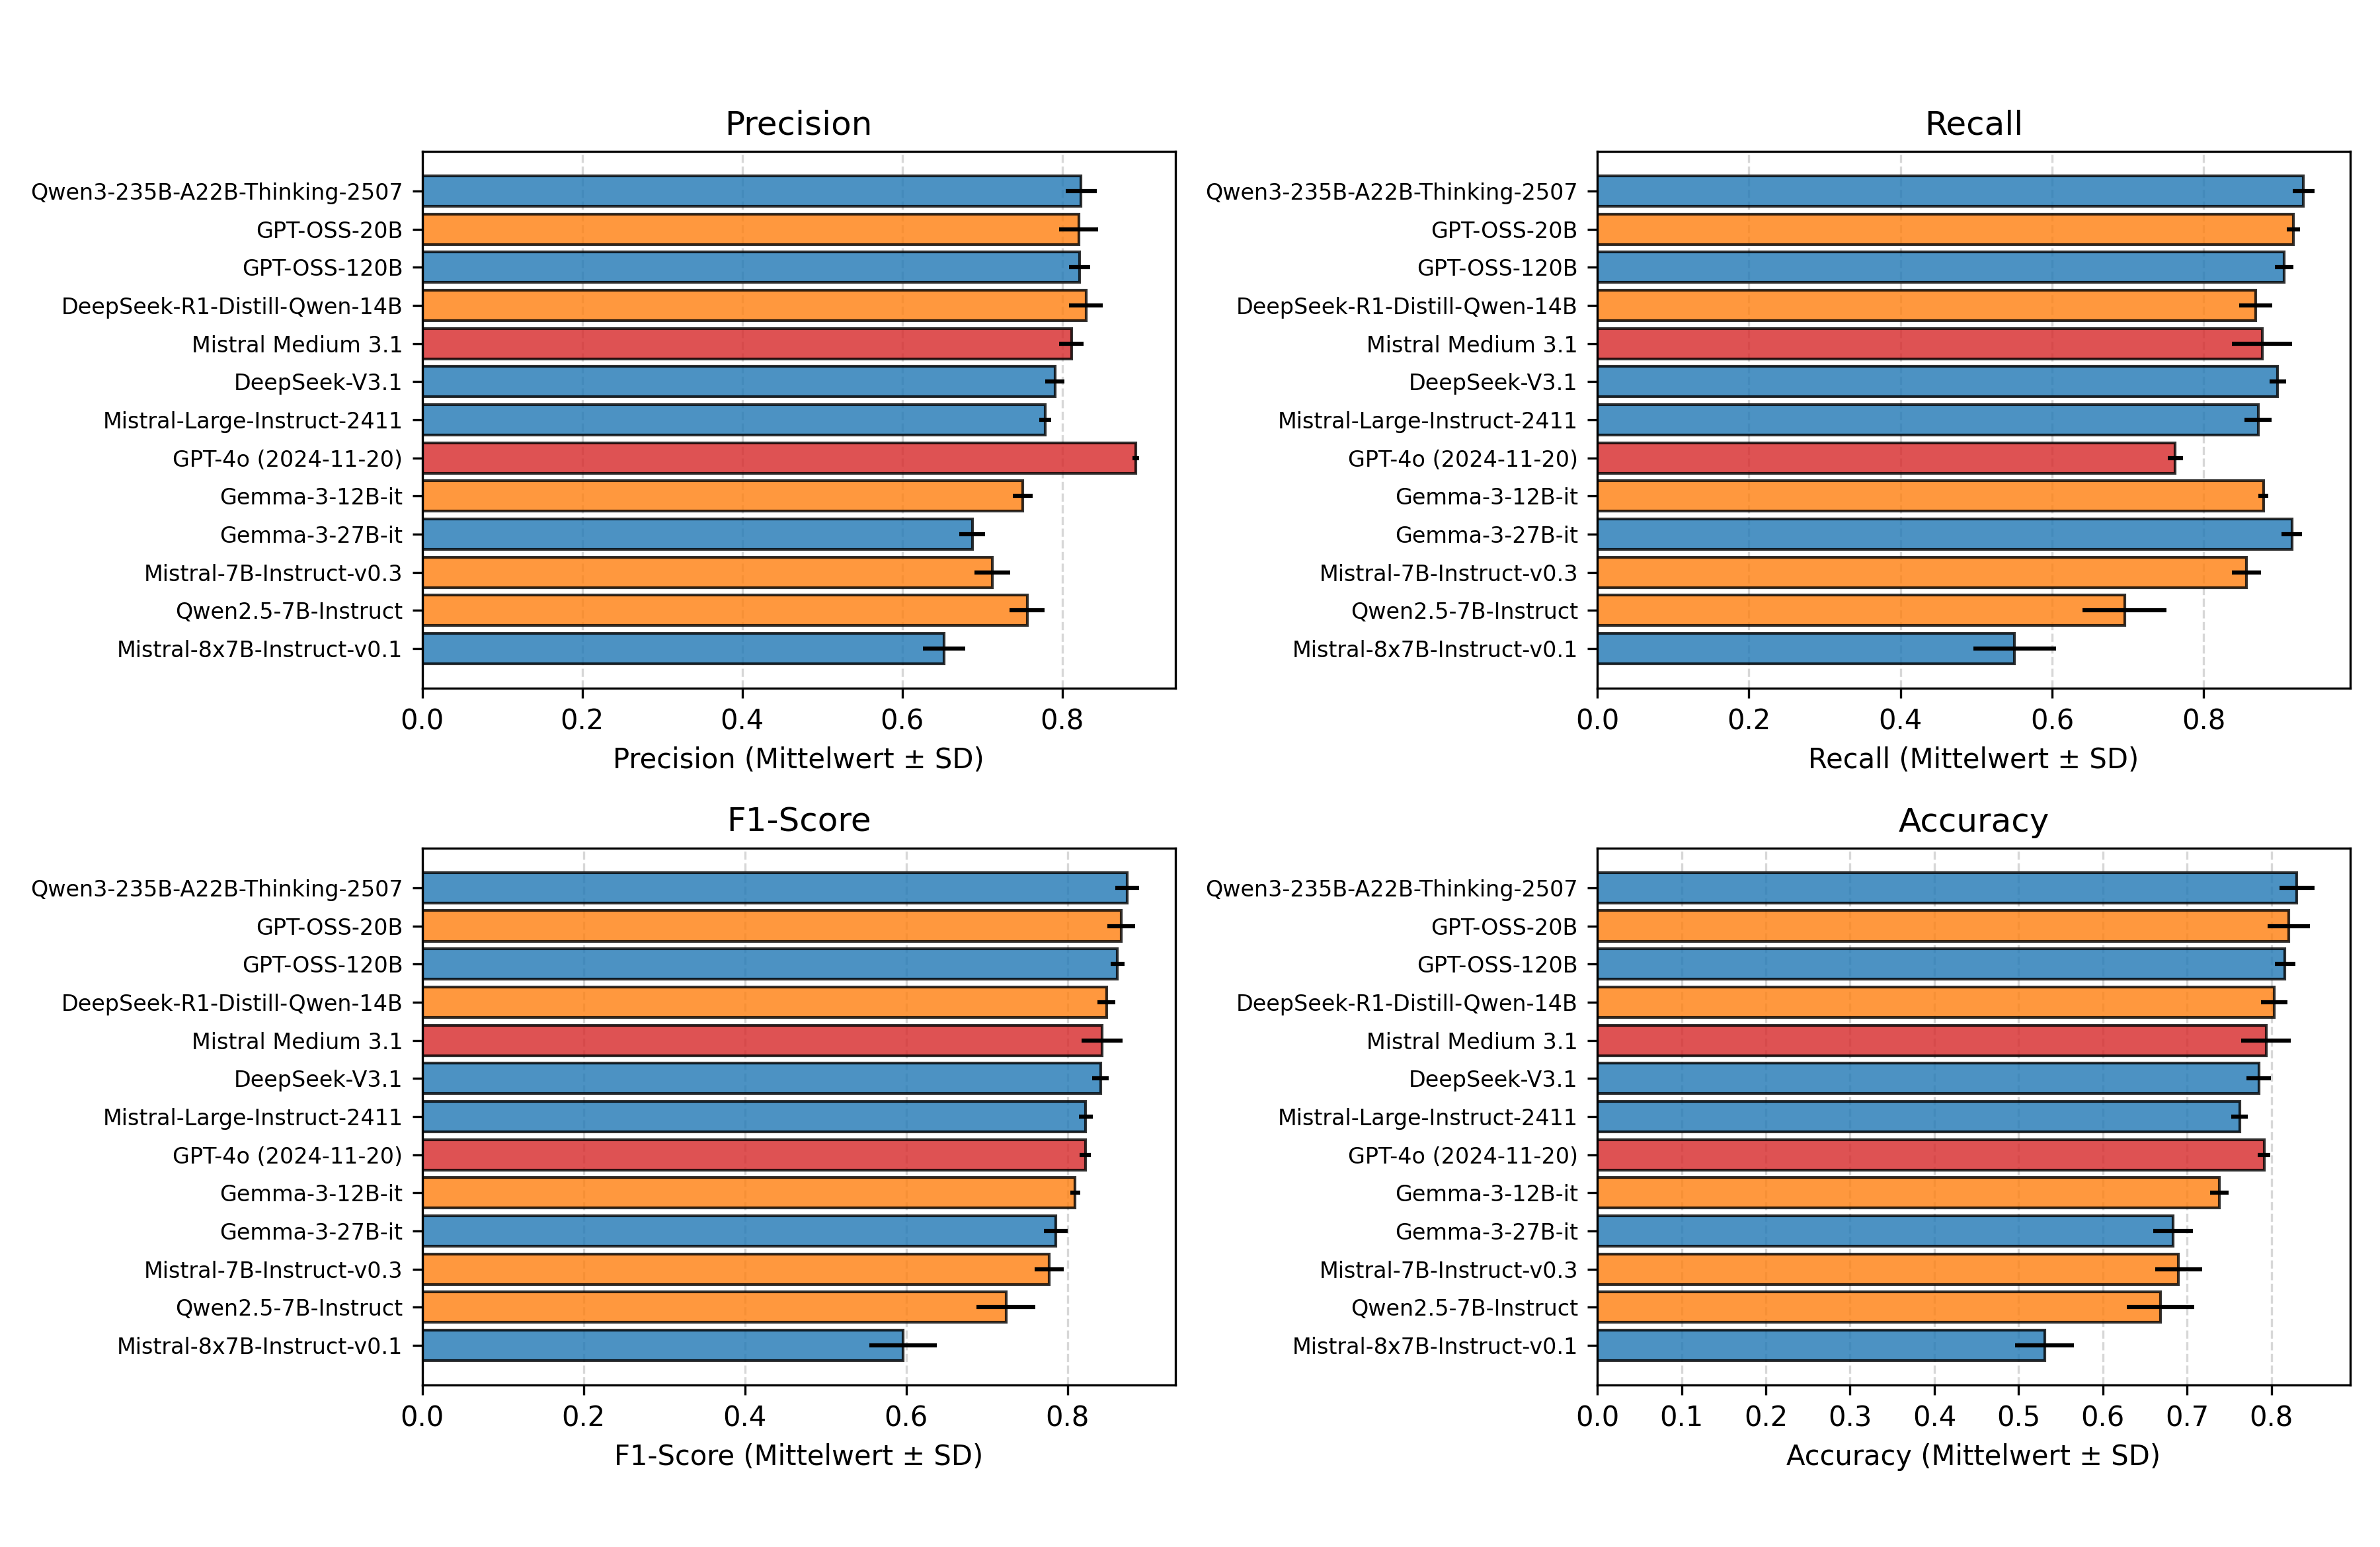
\includegraphics[width=\textwidth]{images/results/evaluation_metrics_comparison}
    \caption{Durchschnittliche Werte für Precision, Recall, F1-Score und Accuracy der untersuchten Modelle über alle Wiederholungen hinweg inklusive Standardabweichung.}
    \label{fig:results-evaluation-metrics-comparison}
\end{figure}

Für die Einordnung der Ergebnisse ist entscheidend, wie Precision und Recall zu interpretieren sind: Ein höherer \emph{Recall} bedeutet, dass ein Modell nur wenige kritische Aktivitäten übersieht (wenige \ac{FN}) und eignet sich damit besonders gut als vorsorgliches \emph{Screening}. Eine höhere \emph{Precision} zeigt dagegen, dass selten unkritische Aktivitäten fälschlich als kritisch markiert werden (wenige \ac{FP}), sodass der manuelle Prüfaufwand sinkt. Der \emph{F1-Score} als harmonisches Mittel aus Precision und Recall fasst beide Perspektiven zu einer Kennzahl zusammen: Er steigt nur dann, wenn \emph{beide} Werte hoch sind, und bestraft Ungleichgewichte (z.\,B. sehr hohe Precision bei niedrigem Recall). Entsprechend setzen die Qualitätsziele in Abschnitt~\ref{sec:qualitatsziele} einen F1-Score $\geq 0{,}80$ als Maß für die kombinierte Screening-Leistung, priorisieren aber den Recall, um das Übersehen kritischer Aktivitäten zu vermeiden. Vor diesem Hintergrund lassen sich die in Abbildung~\ref{fig:results-evaluation-metrics-comparison} sichtbaren Unterschiede zwischen den Modellen einordnen und erklären.

Insgesamt erfüllen neun der dreizehn Modelle den Zielwert eines F1-Scores $\geq 0{,}80$ aus Abschnitt~\ref{sec:qualitatsziele}. Besonders gut schneiden \texttt{Qwen3-235B-A22B-Thinking-2507}, \texttt{GPT-OSS-120B} und \texttt{GPT-OSS-20B} ab, die F1-Scores zwischen $0{,}862$ und $0{,}874$ erreichen. Hervorzuheben ist, dass auch mehrere kleinere Modelle diesen Zielwert überschreiten. Am unteren Ende des Spektrums liegt das europäische \texttt{Mixtral-\linebreak~8x7B-Instruct-v0.1}, das sowohl in Precision als auch in Recall schwach abschneidet und als einziges Modell einen F1-Score deutlich unter $0{,}60$ erzielt.

Die Abbildung zeigt zudem, dass sich die Modelle hinsichtlich Precision und Recall unterschiedlich verhalten. \texttt{GPT-4o} erreicht beispielsweise mit $0{,}892$ die höchste Precision, liegt jedoch beim Recall mit $0{,}762$ unter dem Mindestziel von $0{,}80$ - es würde demnach in der Praxis vergleichsweise viele kritische Aktivitäten übersehen. Umgekehrt erzielt \texttt{Gemma-3-27B-it} einen sehr hohen Recall von $0{,}916$, wird aber durch eine niedrige Precision von $0{,}687$ ausgebremst. Dadurch klassifiziert es viele unkritische Aktivitäten fälschlich als kritisch, was den manuellen Prüfaufwand erhöhen würde. Modelle wie \texttt{Qwen3-235B-A22B-Thinking-2507}, \texttt{GPT-OSS-20B} und \texttt{DeepSeek-R1-Distill-Qwen-14B} bieten eine ausgewogene Balance und zählen deshalb zu den Spitzenreitern.

Tabelle \ref{tab:metrics-overview} fasst alle Metriken mit ihren Mittelwerten und Standardabweichungen tabellarisch zusammen. Für die weitere Analyse werden diese Werte nur noch punktuell zitiert, um Wiederholungen zu vermeiden.

\begin{table}[htbp]
    \centering
    \caption{Aggregierte Mittelwerte und Standardabweichungen der Evaluationsmetriken über alle fünf Wiederholungen hinweg.}
    \label{tab:metrics-overview}
    \begin{adjustbox}{width=\textwidth}
        \begin{tabular}{l r r r r}
            \toprule
            Modell                          & Precision         & Recall            & F1-Score          & Accuracy \\
            \midrule
            DeepSeek-V3.1                   & 0,791 $\pm$ 0,012 & 0,897 $\pm$ 0,011 & 0,841 $\pm$ 0,011 & 0,785 $\pm$ 0,015 \\
            DeepSeek-R1-Distill-Qwen-14B    & 0,829 $\pm$ 0,021 & 0,868 $\pm$ 0,022 & 0,848 $\pm$ 0,011 & 0,803 $\pm$ 0,016 \\
            Gemma-3-12B-it                  & 0,751 $\pm$ 0,013 & 0,879 $\pm$ 0,006 & 0,810 $\pm$ 0,006 & 0,738 $\pm$ 0,011 \\
            Gemma-3-27B-it                  & 0,687 $\pm$ 0,016 & 0,916 $\pm$ 0,014 & 0,785 $\pm$ 0,015 & 0,683 $\pm$ 0,023 \\
            Mistral-7B-Instruct-v0,3        & 0,712 $\pm$ 0,022 & 0,856 $\pm$ 0,019 & 0,777 $\pm$ 0,018 & 0,690 $\pm$ 0,028 \\
            Mixtral-8x7B-Instruct-v0,1      & 0,652 $\pm$ 0,027 & 0,550 $\pm$ 0,054 & 0,596 $\pm$ 0,042 & 0,531 $\pm$ 0,035 \\
            Mistral-Large-Instruct-2411     & 0,779 $\pm$ 0,008 & 0,872 $\pm$ 0,018 & 0,823 $\pm$ 0,008 & 0,762 $\pm$ 0,010 \\
            Mistral Medium 3.1              & 0,811 $\pm$ 0,015 & 0,877 $\pm$ 0,040 & 0,843 $\pm$ 0,025 & 0,794 $\pm$ 0,029 \\
            GPT-OSS-20B                     & 0,820 $\pm$ 0,024 & 0,918 $\pm$ 0,009 & 0,866 $\pm$ 0,017 & 0,821 $\pm$ 0,025 \\
            GPT-OSS-120B                    & 0,822 $\pm$ 0,013 & 0,906 $\pm$ 0,012 & 0,862 $\pm$ 0,009 & 0,816 $\pm$ 0,012 \\
            GPT-4o                          & 0,892 $\pm$ 0,004 & 0,762 $\pm$ 0,010 & 0,822 $\pm$ 0,007 & 0,791 $\pm$ 0,007 \\
            Qwen2.5-7B-Instruct             & 0,756 $\pm$ 0,022 & 0,696 $\pm$ 0,055 & 0,724 $\pm$ 0,037 & 0,668 $\pm$ 0,040 \\
            Qwen3-235B-A22B-Thinking-2507   & 0,824 $\pm$ 0,019 & 0,932 $\pm$ 0,014 & 0,874 $\pm$ 0,015 & 0,830 $\pm$ 0,021 \\
            \bottomrule
        \end{tabular}
    \end{adjustbox}
\end{table}

Neben den zusammengeführten Metriken wurden die 25 Testfälle je Modell auch hinsichtlich der Frage ausgewertet, wie viele Testfälle das Modell bestanden hat. Ein Testfall gilt als bestanden, wenn alle \ac{DSGVO}‑kritischen Aktivitäten korrekt klassifiziert und keine unkritischen Aktivitäten fälschlicherweise als kritisch markiert wurden. Schlägt ein Testfall fehl, liegt mindestens eine Fehlklassifikation (\ac{FP} oder \ac{FN}) vor. Daneben gab es wenige technische Fehler, etwa Parsing‑Fehler oder Timeouts, die selbst nach dem in Abschnitt  \ref{sec:validierung-der-ausgabe} beschriebenen Retry‑Mechanismus nicht behoben werden konnten. Diese technischen Fehler wurden, wie in Abschnitt \ref{sec:scope-und-annahmen} festgehalten, nicht in die Metriken einbezogen und sind hier separat ausgewiesen.

\begin{figure}[htbp]
    \centering
    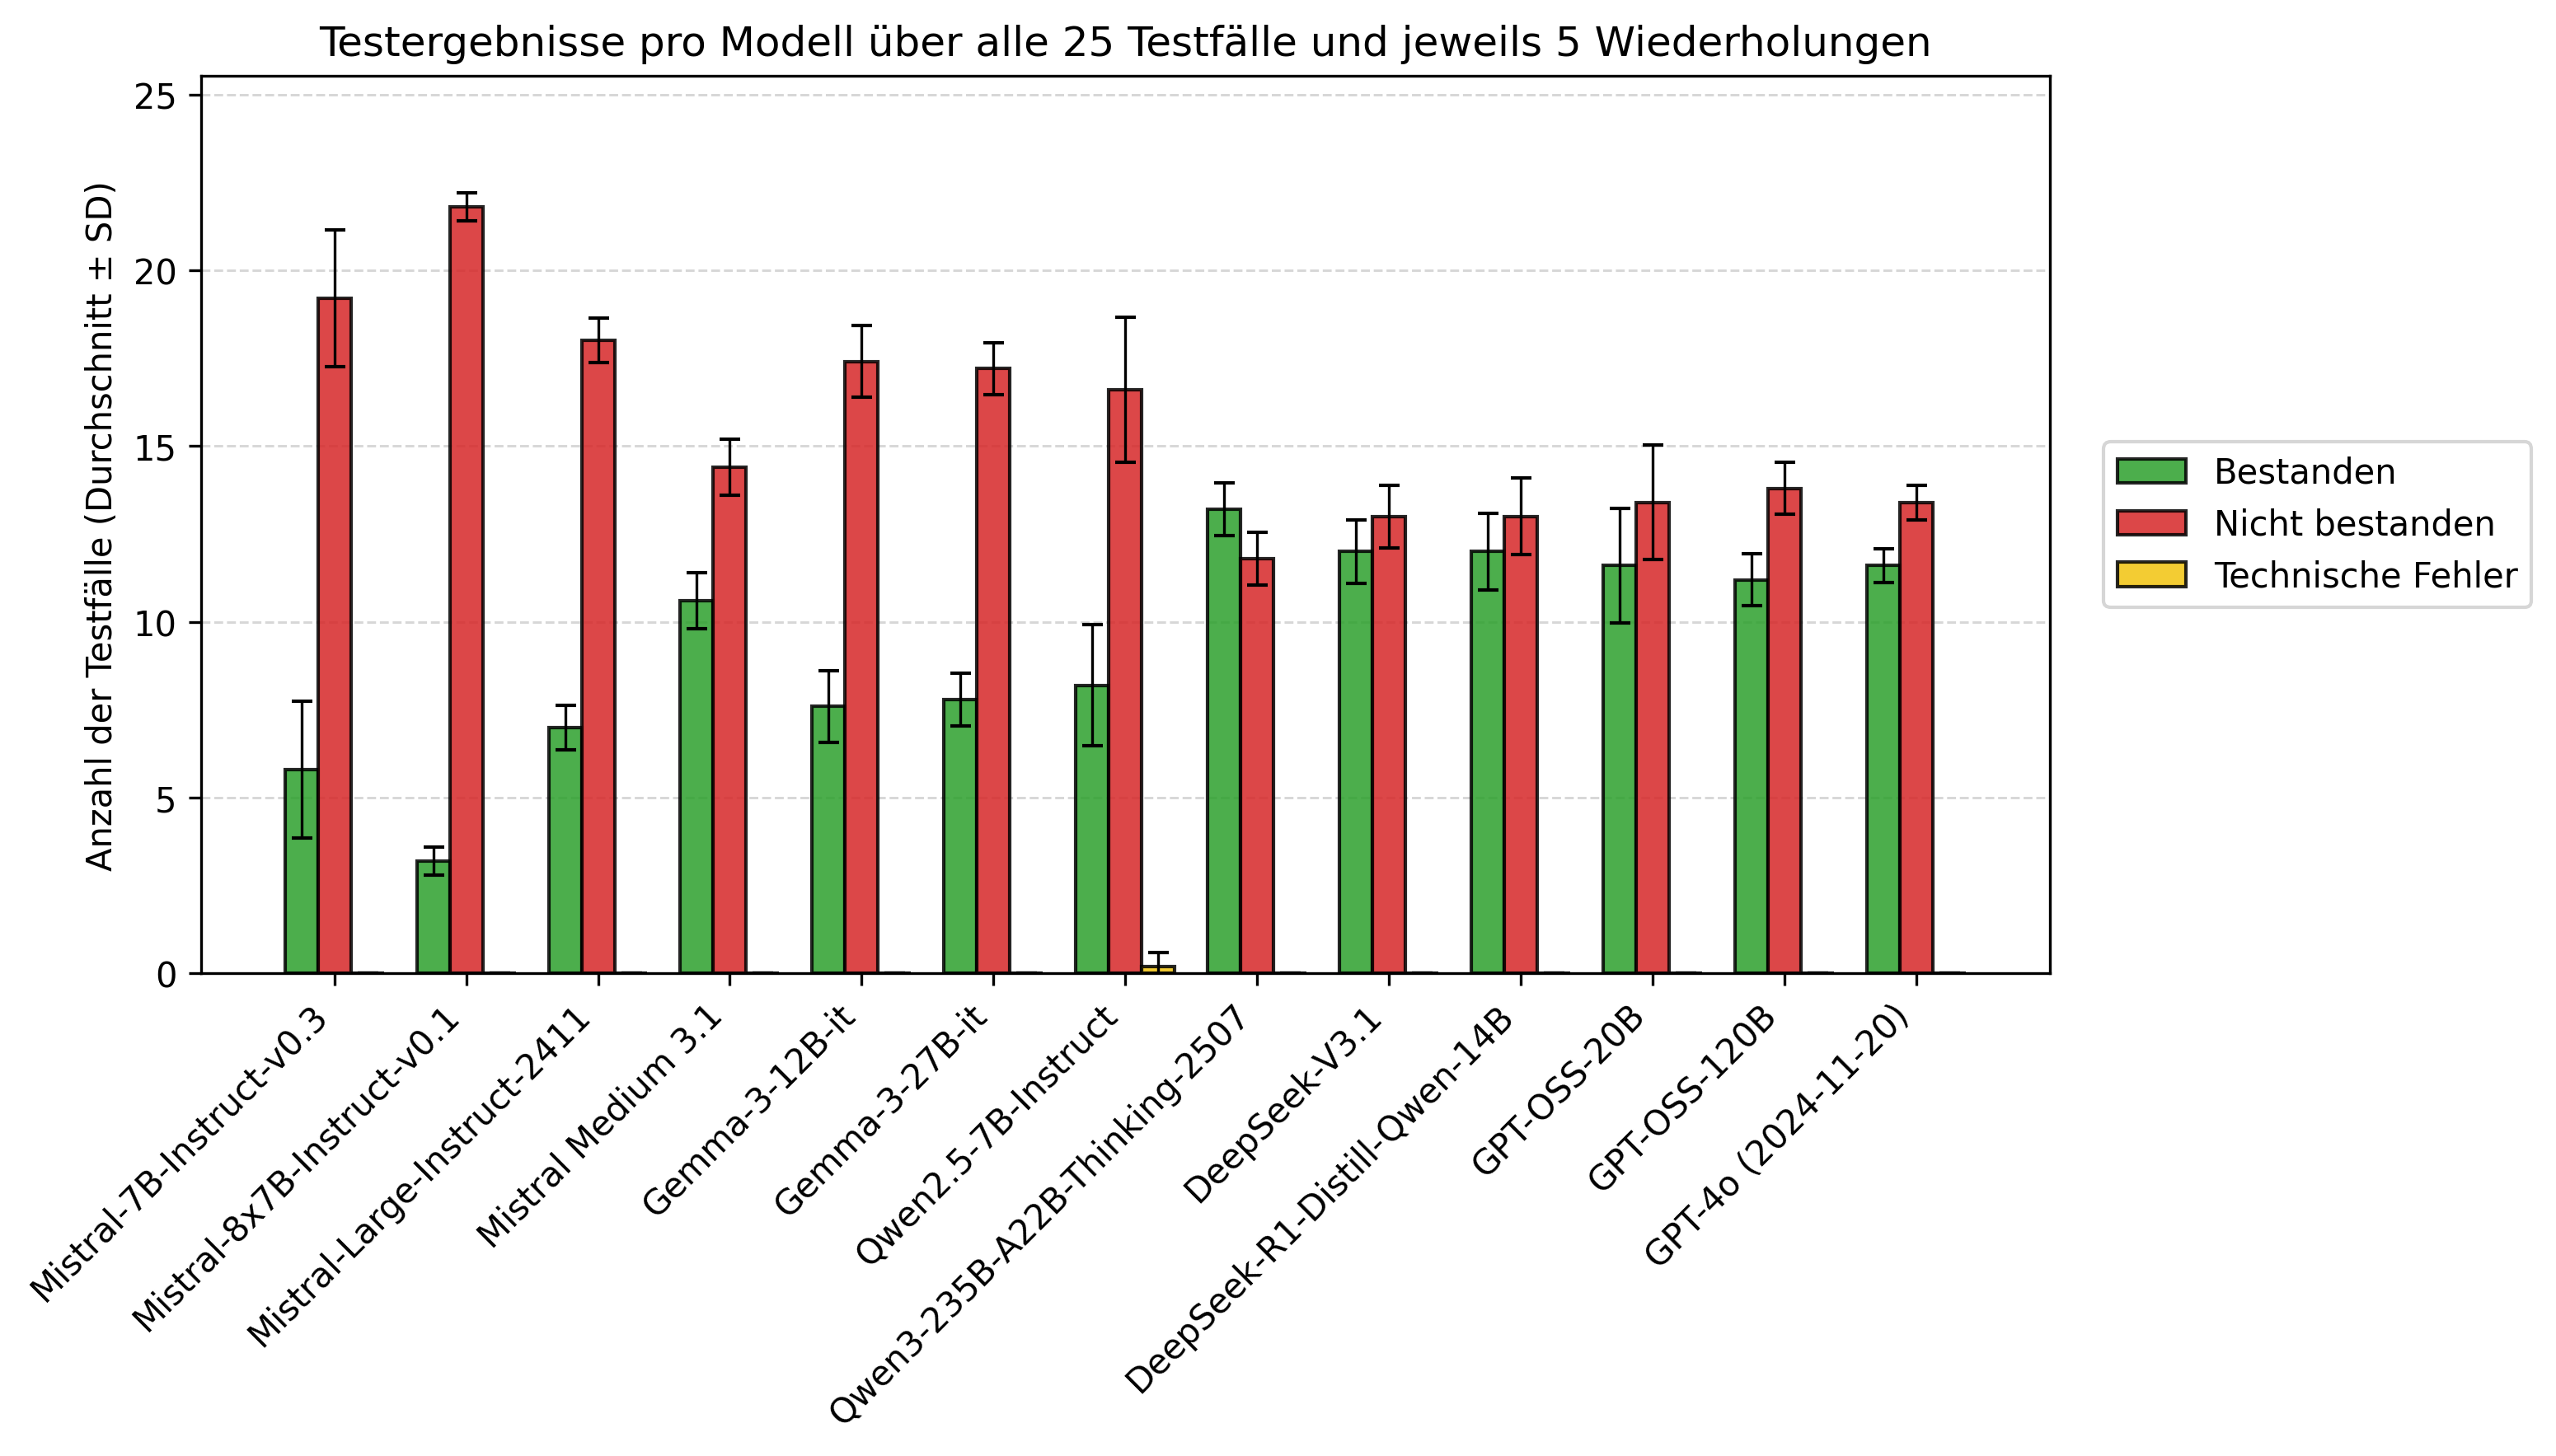
\includegraphics[width=\textwidth]{images/results/evaluation_testcase_outcomes_grouped}
    \caption{Durchschnittliche Testergebnisse pro Modell in Bezug auf die 25 Testfälle über fünf Wiederholungen hinweg.}
    \label{fig:results-testcase-outcomes}
\end{figure}

Wie Abbildung \ref{fig:results-testcase-outcomes} zeigt, korrespondieren die Ergebnisse der Testfälle weitgehend mit den Metriken aus \autoref{tab:metrics-overview}. Modelle wie \texttt{Qwen3-235B-A22B-Thinking-\linebreak~2507}, \texttt{DeepSeek-V3.1} und \texttt{GPT-OSS-20B} bestehen im Durchschnitt fast die Hälfte der Testfälle, während \texttt{Mistral-7B-Instruct-v0.3} und \texttt{Mistral-8x7B-\linebreak~Instruct-v0.1} die meisten Testfälle verfehlen. Auffällig ist, dass \texttt{Qwen2.5-7B-\linebreak~Instruct} als einziges Modell vereinzelte technische Fehler zeigte. Dabei ging es um Parsing-Fehler. Diese treten jedoch selten auf und haben keinen Einfluss auf die berechneten Metriken. Insgesamt bestätigt die Testfallanalyse, dass die leistungsstärksten Modelle nicht nur hohe Metrikwerte erzielen, sondern auch die meisten Testfälle bestehen.
\chapter{Aussicht}

Unter anderem das hier, evtl noch mehr:
\begin{itemize}
    \item Jetzt gibt es ein einheitliches Evaluationsframework mit einer einheitlich definierten Schnittstelle für Klassifizierungsalgorithmen -> Zukünftige Arbeiten können sich mit der Entwicklung besserer Klassifizierungsalgorithmen/Pipelines (Bspw. noch RAG einbauen) beschäftigen und diese mit diesem Framework vergleichen/benchmarken
    \item Außerdem können in Zukunft auch noch mehr Modelle vergleichen werden, da sich die Welt der LLMs rasant weiterentwickelt
    \item Auch Finetunen ist etwas was interessant gewesen wäre für diese Masterarbeit, aber den Rahmen gesprengt hätte
\end{itemize}


\appendix
% hier Anhänge einbinden
\chapter{Quelltexte}\label{ch:quelltexte}

In diesem Anhang sind mehrere Quellcode-Ausschnitte aufgeführt.

\begin{lstlisting}[caption={System-Prompt fuer die DSGVO-Klassifikation von BPMN-Aktivitäten},label={lst:system-prompt}]
You are an expert in analysing Business Process Model and Notation (BPMN) diagrams for GDPR compliance. Your task is to identify and return a list of the IDs of all Activity (Task) elements that process personal data. Ignore all other element types. Always consider every activity in the process; do not omit any activity from your assessment.

Use all available context for each activity - including the activity's name, description, annotations, associated data objects, and message or data associations - to determine whether the activity processes personal data. Under Article 4 of the GDPR, personal data is any information relating to an identified or identifiable natural person, including names, addresses, email addresses, phone numbers, identification numbers, payment or bank details, employment records, academic records, location data, IP addresses, online identifiers, images, audio/video recordings, biometric identifiers, health data or other information that can be linked to a specific person. "Processing" includes any operation performed on personal data, such as collecting, recording, organising, structuring, storing, retrieving, consulting, using, analysing, transmitting, printing, disseminating, aligning, combining, altering, restricting, erasing or destroying the data.

Classify an activity as GDPR-relevant whenever it performs or enables processing of personal data. Indicators include (but are not limited to):

- **Collection and entry of personal data**: Activities that collect or capture personal information, for example entering contact details, addresses, payment information, job applications, health information, student enrolments, membership data, tax declarations, registration forms or other forms with personally identifiable information.
- **Creation, storage and updating of records**: Activities that create, save or update records containing personal data, such as opening customer accounts, storing order or appointment details, creating personnel files, enrolling students, setting up insurance cases or filing a medical record.
- **Transmission or disclosure of personal data**: Activities that send, print or otherwise disclose personal data to another participant, system or third party. Examples include printing shipping labels or prescriptions, sending orders or personal data to logistics partners, pharmacies, insurers or authorities, generating payroll reports for external providers, notifying universities about student records, transmitting tax or social security data, sending confirmations or queries that rely on a person's contact details, or transferring data to non-EU locations.
- **Payments and financial transactions**: Activities that process personal financial data, such as initiating or verifying payments, processing bank account or credit-card information, executing payroll, handling reimbursements or insurance payouts, managing expense claims or collecting membership fees.
- **Use of health, biometric or other special categories of data**: Activities that handle medical diagnoses, prescriptions, insurance claims, disability information, photos of damages or patients, biometric identifiers (fingerprints, facial images, voice), racial or ethnic data, political opinions, religious beliefs or union membership. Processing these "special categories" always triggers GDPR relevance.
- **Audio/Video and communications**: Activities that initiate or join audio or video calls, record calls or meetings, capture surveillance footage, or communicate directly with a data subject via email, chat, SMS or other channels. Simply using a person's contact data to send reminders, marketing messages or notifications is processing.
- **Profiling, scoring and decision-making**: Activities that analyse or evaluate a person's performance, behaviour or characteristics for purposes such as credit scoring, hiring, admissions, insurance underwriting, marketing segmentation, customer value analysis or automated decision-making.
- **Logging, tracking and location data**: Activities that log user activity, record access or usage data, track geolocation (e.g. telematics, fleet or mobile tracking), monitor attendance or timekeeping, or collect IP addresses or device identifiers.
- **Consent and data-subject rights**: Activities that obtain, record or manage consent; respond to requests for access, rectification, restriction, erasure, data portability or objections; or document lawful bases for processing.
- **Deletion, anonymisation or pseudonymisation**: Activities that erase, anonymise or pseudonymise personal data, even if the goal is to remove identifiers, because these operations manipulate personal data.

When assessing an activity, consider synonyms or domain-specific terms: activities referring to customers, patients, applicants, employees, students, voters, taxpayers, residents or members often imply personal data processing, even if names like "address" or "contact" are absent. Use context - data objects, annotations or typical process semantics - to infer personal data involvement. Do not rely solely on explicit data-object links; many process names ("Anmeldung pruefen", "Aufnahmeantrag bearbeiten", "Kundeninfo aktualisieren", "Registrierung bestaetigen", "Kreditwuerdigkeit berechnen") themselves indicate personal data processing.

Do **not** classify an activity as GDPR-relevant when it only performs administrative or logistic tasks that do not involve personal data. Examples include picking or packing goods, routing vehicles without using specific addresses, printing generic pick lists, moving items in inventory, or checking if a document exists without viewing its contents. Likewise, activities using truly aggregated or irreversibly anonymised data can be ignored if no individual can be reidentified.

In your output, return only the IDs of activities you classify as GDPR-relevant. For each, provide a clear explanation using the activity's name and description to justify why it processes personal data. Do not reference element IDs in your explanation; use the activity names instead. Exclude from your result any activities that do not process personal data and any elements that are not activity/task elements.
\end{lstlisting}

\begin{lstlisting}[language=Kotlin,caption={Antworttyp fuer die Klassifizierung},label={lst:bpmn-analysis-result}]
data class BpmnAnalysisResult(
    @Description("List of Activity Elements that are classified as relevant for GDPR compliance")
    var elements: List<Element>
) {

    init {
        elements = elements.filter { it.isRelevant }
    }

    @Description("Represents an Activity/Task Element that is classified as relevant for GDPR compliance")
    data class Element(
        @Description("The ID of the Activity Element")
        val id: String,
        @Description("The detailed reason why the Activity Element is relevant for GDPR compliance and why you think personal data is processed.")
        val reason: String,
        @Description("Indicates whether the Activity Element is relevant for GDPR compliance")
        val isRelevant: Boolean = true
    )

    /* Andere Methoden dieser Klasse sind weggelassen */
}
\end{lstlisting}

\begin{lstlisting}[caption={Schema der YAML-Evaluationskonfiguration},label={lst:evaluation-config-schema}]
{
    "$schema": "https://json-schema.org/draft/2020-12/schema",
    "$ref": "#/definitions/Configuration",
    "definitions": {
        "Configuration": {
            "type": "object",
            "additionalProperties": false,
            "properties": {
                "defaultEvaluationEndpoint": {
                    "type": "string"
                },
                "maxConcurrent": { "type": "integer" },
                "models": {
                    "type": "array",
                    "items": { "$ref": "#/definitions/Model" }
                },
                "datasets": {
                    "type": "array",
                    "items": { "type": "integer" }
                },
                "seed": { "type": "integer" }
            },
            "required": [
                "defaultEvaluationEndpoint",
                "models"
                "datasets",
            ],
            "title": "Configuration"
        },
        "Model": {
            "type": "object",
            "additionalProperties": false,
            "properties": {
                "label": { "type": "string" },
                "evaluationEndpoint": { "type": "string" },
                "llmProps": { "$ref": "#/definitions/LlmProps" }
            },
            "required": [ "label" ],
            "title": "Model"
        },
        "LlmProps": {
            "type": "object",
            "additionalProperties": false,
            "properties": {
                "baseUrl": {
                    "type": "string",
                    "format": "uri",
                    "qt-uri-protocols": [ "https" ]
                },
                "modelName": { "type": "string" },
                "apiKey": { "type": "string"},
                "timeoutSeconds": { "type": "number" }
            },
            "required": [],
            "title": "LlmProps"
        }
    }
}
\end{lstlisting}

\begin{lstlisting}[caption={Zusammengefasster Logauszug zum Retry-Mechanismus}, label={lst:retry-log}]
2025-10-03T19:11:51.152+02:00  INFO  BpmnExtractor  : Extracting BPMN elements from XML

# 1) Erste Anfrage an das LLM (gekuerzt: Prompt/Headers/Body)
2025-10-03T19:11:51.156+02:00  INFO  LoggingHttpClient  : HTTP POST https://openrouter.ai/api/v1/chat/completions
  model: openai/gpt-oss-20b
  messages: [system: (System-Prompt), user: (User-Prompt mit BpmnElement-Liste und Format-Anweisung)]

# 2) Antwort des LLM mit fehlerhaftem JSON (verkuerzt)
2025-10-03T19:11:56.671+02:00  INFO  LoggingHttpClient  : HTTP 200
assistant:
{
  "elements": [
    { "id": "Activity_09ehuii", "reason": "...", "isRelevant": true },
    { "id": "Activity_1la5hsp", "reason": "...", "isRelevant":  }   <-- fehlender Bool-Wert
    { "id": "Activity_0rfgrlm", "reason": "...", "isRelevant": true }
  ]
}

# 3) Parser-Fehler + Retry-Ankuendigung (gekuerzt)
2025-10-03T19:11:56.691+02:00  WARN  SafetyNet  : Parsing failed. Attempting to fix JSON and retry... (Attempt 1 of 2)
dev.langchain4j.service.output.OutputParsingException:
  Caused by: com.fasterxml.jackson.core.JsonParseException:
  Unexpected character ('}') ... at elements[1].isRelevant

# 4) Zweite Anfrage zum beheben des JSON mit Chat-Verlauf und Fehlermeldung (n-mal wiederholt, bis erfolgreich)
2025-10-03T19:11:56.721+02:00  INFO  LoggingHttpClient  : HTTP POST https://openrouter.ai/api/v1/chat/completions
  messages: [
    system: (System-Prompt),
    user: (User-Prompt mit BpmnElement-Liste und Format-Anweisung),
    assistant: (Fehlerhafte JSON-Antwort),
    system: (Fix-JSON System-Prompt),
    user: (Fehlermeldung)
  ]

# 5) Korrigierte JSON-Antwort des LLM
2025-10-03T19:12:01.519+02:00  INFO  LoggingHttpClient  : HTTP 200
assistant:
{
  "elements": [
    { "id": "Activity_09ehuii", "reason": "...", "isRelevant": true },
    { "id": "Activity_1la5hsp", "reason": "...", "isRelevant": true }, <-- jetzt mit Bool-Wert
    { "id": "Activity_0rfgrlm", "reason": "...", "isRelevant": true }
  ]
}

# 6) Erfolgreiches Parsing und Weiterverarbeitung
2025-10-03T19:12:01.519+02:00  INFO  PromptBpmnAnalyzer : BPMN Analysis Result: elements=[... isRelevant=true ...]
\end{lstlisting}

\backmatter
\nocite{Knappen2009}
\nocite{Mittelbach2005}
\nocite{Schlosser2014}
\nocite{Sturm2012}
\nocite{Voss2010}

\printbibliography

\clearpage
\thispagestyle{empty}

Name: \fullname \hfill Matrikelnummer: \matnr \vspace{2cm}

\minisec{Erklärung}

Ich erkläre, dass ich die Arbeit selbständig verfasst und keine anderen als die angegebenen Quellen und Hilfsmittel verwendet habe.\vspace{2cm}

Ulm, den \dotfill

\hspace{10cm} {\footnotesize \fullname}
\end{document}
